% Class
\documentclass[a4paper,11pt]{report}

% Packages
\usepackage[table]{xcolor}
%\usepackage[utf8]{inputenc}

\usepackage[left=1.25in, 
right=1in, 
top=1in, 
bottom=1in, 
includefoot, 
includehead]{geometry}

\usepackage{float}
\usepackage{enumerate}
\usepackage{algorithm}
\usepackage{tabularx}
\usepackage{algorithmic}
\usepackage{array}
\usepackage{amssymb}
\usepackage{amsmath}
\usepackage{color}
\usepackage{fancyhdr}
%\usepackage{fontspec}
\usepackage{graphicx}
\usepackage{placeins}
\usepackage{listings}
\usepackage{supertabular}
\usepackage{wasysym}
\usepackage{colortbl}
\usepackage{tikz}
\usepackage{pgfplots}
\usepackage{pgf-umlsd}
\usepackage{scrextend}
\usepackage{svg}
\usepackage[draft]{todonotes}
\usepackage{lastpage}
%\usepackage{hyperref}
\usetikzlibrary{positioning, fit, calc, shapes, arrows, shadows}

\setcounter{tocdepth}{4}
\setcounter{secnumdepth}{4}

\graphicspath{ {images/} }

\renewcommand{\thesection}{\arabic{section}}

\renewcommand\headrulewidth{0.5pt}
\renewcommand\footrulewidth{0.5pt}

% Style
\parskip=\smallskipamount
\def\ieme{\up{\lowercase{\`eme}}\ }

% Langages
\definecolor{grey}{rgb}{0.96,0.96,0.96}
\definecolor{midgrey}{rgb}{0.70,0.70,0.70}

\lstset{
numbers=left,
numberstyle=\tiny,
stepnumber=1,
numbersep=10pt,
aboveskip=\bigskipamount,
basicstyle=\scriptsize\ttfamily,
numberstyle=\tiny\ttfamily,
frame=single,
backgroundcolor=\color{grey},
rulecolor=\color{black}}

\lstdefinelanguage{metalangage}{
keywords=[1]{begin,do,end,fi,function,goto,if,od,procedure,record,
type,var},
    %keywords=[2]{char,integer,boolean,real,single,double,extended,text,
    %             false,nil,true,and,array,as,cand,cor,div,file,in,label,
    %             mod,not,of,or,skip},
    otherkeywords={->,[],^},
    keywordstyle=[1]\underbar,
    morecomment=[l]{//},
    morecomment=[s]{\{}{\}},
    sensitive=true,
    literate={->}{$\rightarrow$}1 
    {^}{$\uparrow$}1 
    {!=}{$\neq$}1 
    {<=}{$\leq$}1 
    {>=}{$\geq$}1 
    {[]}{$\Box$}2}

% URLs
\usepackage{url}
\numberwithin{figure}{section} % Number figures within sections (i.e. 1.1, 1.2, 2.1, 2.2 instead of 1, 2, 3, 4)

\makeatletter
\def\url@leostyle{%
\@ifundefined{selectfont}{\def\UrlFont{\sf}}{\def\UrlFont{\small\ttfamily}}}
\makeatother
\urlstyle{leostyle}

% Headers
\lhead{\textbf{INFO-8006}}
\rhead{\textbf{Introduction to AI}}
\chead{}

\lfoot{}
\rfoot{}
\cfoot{Page \thepage}

% First Page
\title{
\LARGE
\textbf{New Cytomine modules for user behavior analytics in digital pathology}\\
\vspace{1cm}
Master Thesis\\
\vspace{0.3cm}
Academic year 2017-2018\\
University of Li\`{e}ge - Faculty of Applied Sciences\\
\vspace{3cm}

\includegraphics[scale=0.75]{logo.jpg}
\vspace{2cm}
}
\author{ Graduation Studies conducted for obtaining the Master's degree in \\Computer Sciences by Laurent Vanhee}
\date{June 2018}

\pgfplotsset{compat=1.14}
\usepackage[T1]{fontenc}



\begin{document}
\pagestyle{empty}
\maketitle

\tableofcontents

\pagestyle{fancy}
\fancyhf{}
\rfoot{Page \thepage \hspace{1pt} of \pageref{LastPage}}
\newpage
\section{Abstract}
In the medical field, doctors and researchers need to be able to observe and interpret cell samples.
The
most widely spread method is to observe samples with a microscope.
New methods allow us to scan a
sample into a very large and detailed image.
These images can be uploaded to the Cytomine web
application and doctors can go through the images with ease.
The application includes many
functionalities, namely the ability to annotate regions of interest.
Currently the ULiege MOOC server is
used for the benefit of the students studying the medical field at the University of Liege.
The students
study particular images and are then evaluated at the end of the year.
Meanwhile, the Cytomine app
has been collecting data on the students’ time spent on the website.
The bulk of the data collected
consists of where the students decided to look in the images (Gaze data).
With that, attempts  were made to find correlations between students’ behavior and the results they obtain during exams.
Using Machine
Learning techniques, the goal is to predict a student’s grade based on how they used the application.
Currently, the model contains 395 students with over 2000 features.
Random Forest and Extra Trees
learning techniques have been applied to attempt to predict grades.
Otherwise, another goal is to
visualize these patterns.
The idea would be to generate Heatmaps of the students’ gaze data (Gazemap).
These Gazemaps would be included in the app and users can be given access to this information.
This
could give teachers the ability to keep track of the students’ work.
\section{Introduction}

\subsection{Cytomine}


\begin{center}
    
\includegraphics[scale=0.80]{logo_cytomine.jpg}
\end{center}

Open-source rich Internet application for collaborative analysis of multi-gigapixel images.
Cytomine can be described by three main properties :
\begin{itemize}
\item[\textbullet] Open Source : The source code is available to the general public, in this case with Github.
It has an Apache 2.0 License, which is very permissive for any third party.
It is also accompanied by documentation that describes the different modules and how to use them.
\item[\textbullet] Open Company : It's a non-profit company that contribute and promote the project.
\item[\textbullet] Open Research : Cytomine employs researchers at the Montefiore Institute of the University of Liege.
They develop Machine Learning algorithms, image informatics, and Big Data modules.
Cytomine also collaborates with other researchers.
\end{itemize}

Cytomine was developed to ease the analysis of multi-gigapixel images.
These images can take Gigabytes of disk space.
For most computers, displaying such images at full resolution is impossible.
With Cytomine, images are stored in a server.
These images can be viewed using the web application with any modern browser.
Cytomine handles everything locally so that performance is not an issue for the clients.\\

	Cytomine also comes with a comprehensive and robust API (Application Programing Interface).
	This API allows clients to fetch and send data to and from a Cytomine Server.
	This is very useful for data analysis, it's well organized so that researchers can find what they are looking for.
	There are also tools included that eases certain aspects of handling big data.
	For examples image annotations allows the user to create zones of interest.
	These zones can share characteristics and using learning algorithms, researchers can learn new zones of interest.

\subsection{Cytomine for education}

Cytomine can be used as a tool of education for many subjects.
Since it's open source and well documented, it is possible to fork it and develop new methods and modules.
This can be done for many fields in computer sciences including Machine Learning, Vision, Big Data, or even front-end programing.\\

This is not limited to the field of Computer Sciences.
Fields that require the use of large high definition images can benefit from using Cytomine.
This includes astrology where, people can learn about planets and stars using imagery.
Other sectors include Geology, Art, and in this case Medicine.


\subsection{MOOC Server}

The MOOC server is a Cytomine Web Application used for education by the Faculty of Medicine at the University of Liege.
It is used for the HISL0541 (General histology and alternative experimentation methods that do not use animals) course.
This course is organized for students enrolled for a Bachelor in Medicine.
Students have to study tissue samples. \\

Cytomine is a great tool for this particular field because it can be used to store and display high quality images of tissue samples.
It is also easily accessible for the students, they are not restricted to only using it during lab sessions.
It's available 24 hours a day, therefore it gives students a good amount of liberty.
The details of the assignments are given by Ecampus which is communication tool for students and teachers delivered by the University.
The teachers can also use Cytomine to explain certain visual concepts in real-time.
They can also use certain images for exercises by telling students to find patterns in those images.\\

Since the MOOC is completely integrated to the course, it directly impacts how students learn.
Their exams are often based on what they learned using the tool.
The goal is to see how much of an effect Cytomine has on students.

%todo subject to change
\subsection{Teachers' Opinion of the Tool}

\subsection{General Goals}


    The Main objective is to observe how the students use Cytomine.
    Since Cytomine is still in development, an objective is to make it robust and user friendly.
    This analysis can give some insight on what works well and what doesn't.
    As a follow up, it would be interesting to see the patterns that that can be observed in regards to the user.
    The teachers also provided some information on students that followed the course.
    This includes the grade obtained and all the tests that lead to that final grade.
    With this information, machine learning can be used to analyze these grades and what patterns lead to them.
    This analysis returns statistics in many forms since there is such a wide range of variables. (Figure \ref{fig:highlevel})

      \begin{figure}[H]
      \centering
      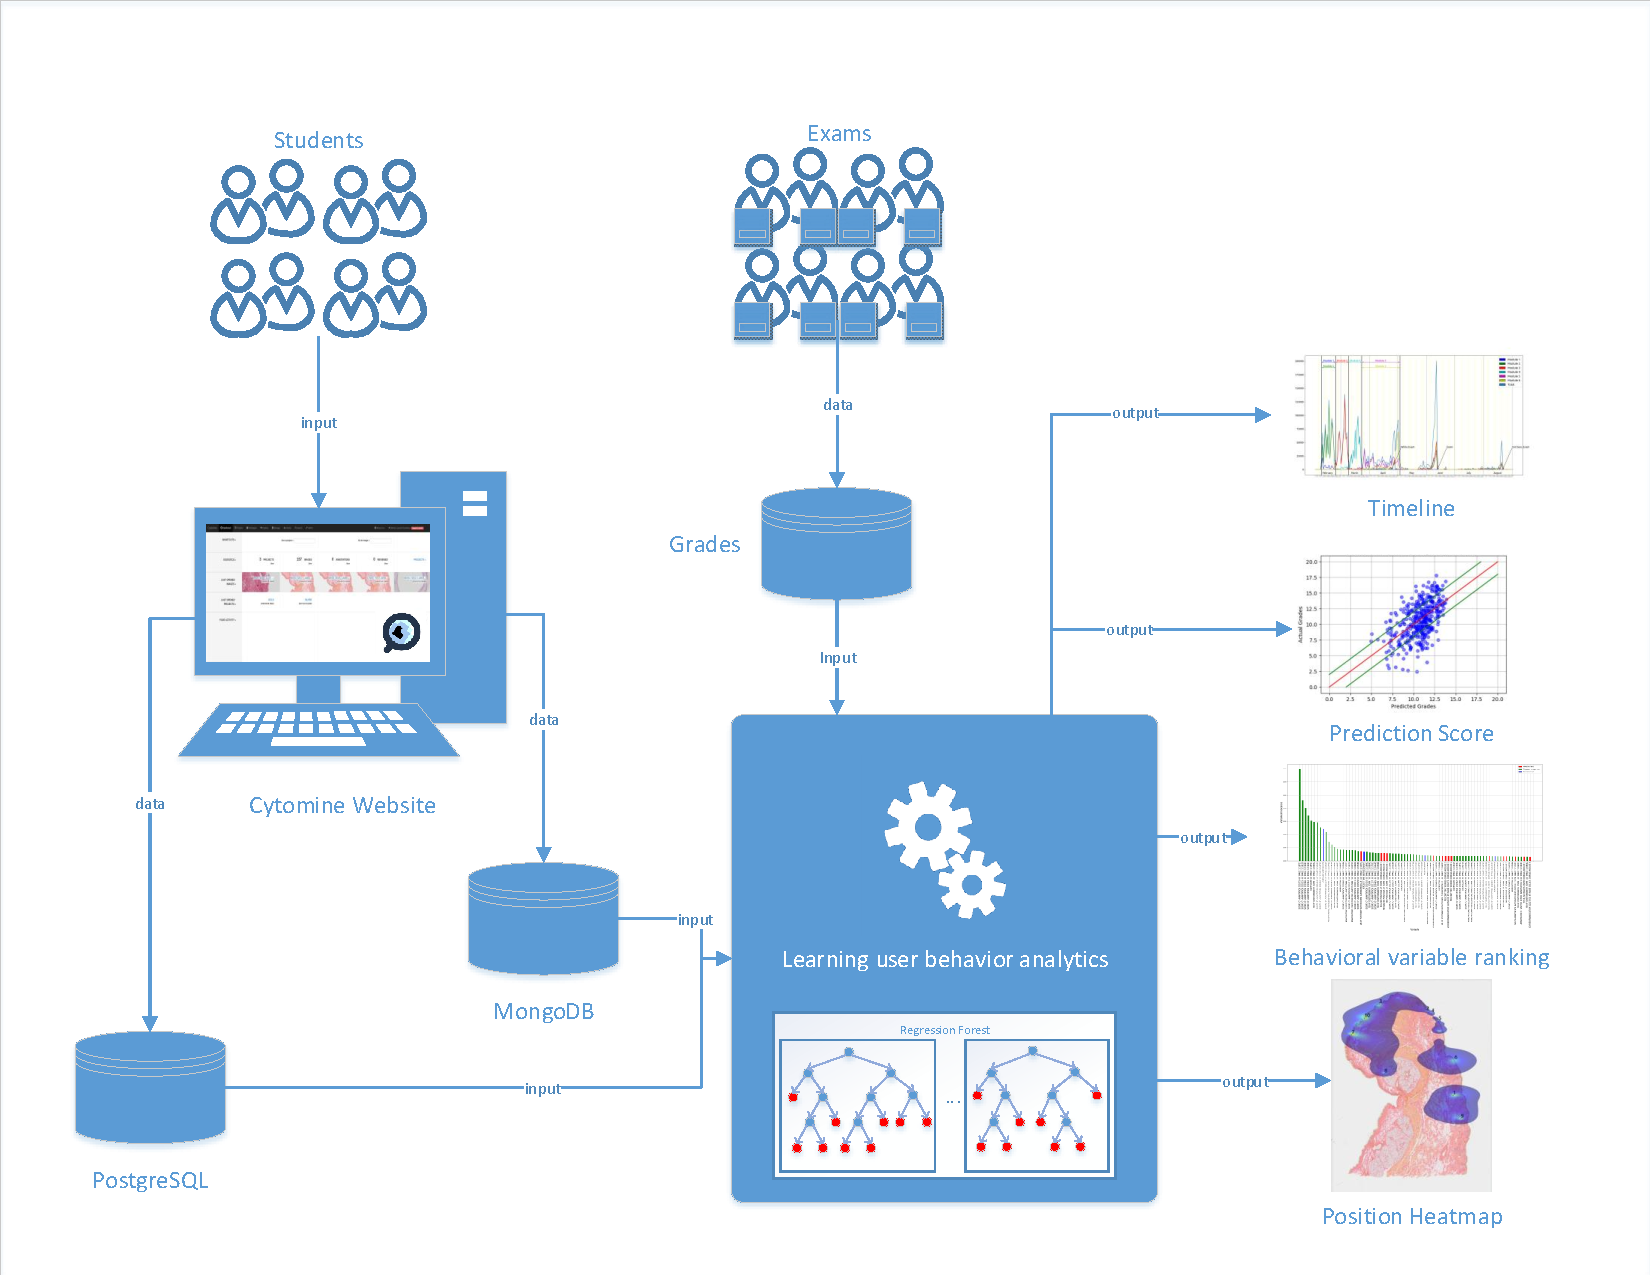
\includegraphics[width=.95\linewidth]{highlevel.pdf}
      \caption{High Level View of the Tool}
      \label{fig:highlevel}
      \end{figure}

\section{Tools and Methods}
	
    \subsection{Three Separate Components}
    	Since there is a vast amount of data, most operations require some good amount of time to complete.
    	Therefore, the data analysis tool is divided into three components :
        \begin{itemize}
        \item[\textbullet] Data Acquisition.
        \item[\textbullet] Data Manipulation.
        \item[\textbullet] Data Learning.
        \end{itemize}

		\subsubsection{Data Acquisition}
        
			During the 2016-2017 Academic year, Cytomine tracked and stored user information on the MOOC server.
			To obtain all this information, Cytomine is accessible by a REST API. To ease the access to the server, Cytomine developed a Python Client that was used for the acquisition of relevant information.
			With administrator rights, a user can get a hold of all if not most of the data stored on the SQL and MongoDB databases.
            
          There are currently a total of two projects called GOLD and SILVER that students could participate in.
          To start of, each project contains a set of images and a set of students that have signed up.
          
          \begin{center}
          \begin{tabular}{| l | c | c |}
          \hline
           & Number Of students & Number Of Images \\ \hline
           GOLD & 395 & 78 \\ \hline
           SILVER & 85 & 75 \\
          \hline
          \end{tabular}
          \end{center}

		  Both projects have their own objectives but GOLD is more complete and thorough.
		  unlike the SILVER project, the students were tested and graded on the course that was given to them but also the content of the project.
         
          To analyze user behavior, it is necessary to fetch data that is relevant, this includes (as shown in Figure \ref{fig:data}):
          
          \begin{itemize}
          \item[\textbullet] Resized images :\newline
          
          The images stored on Cytomine are in fact very large.
          For the analysis, a copy of the images will be useful.
          Many operations in the Data Manipulation component rely on the image resolution when it comes to complexity.
          It is important that the image is big enough to be viewable while small enough so that the operations done in a reasonable amount of time.
          The image downloaded is therefore rescaled to a maximum width and height of 1024 pixels.\\
          \item[\textbullet] Reference Annotations :\newline
          
          When observing images, students are usually given guidelines in forms of image annotations.
          These annotations are zones in the image that contain information that students can learn from.
          These annotations are given a number.
          Annotations from the same image have a different numbers.
          This represents the recommended order the user can traverse the image.
          In this study, only the geometrical center of the annotation is kept.
          In most cases, this loss of information should have no impact because the size of the zones are usually a couple pixels wide when put in the resized image.\\
          %%todo add image with annotations 
		\item[\textbullet]  User Annotations :\newline
        
        Teachers can set annotations as guidelines, but normal users can also create annotations.
        If a student user notices something interesting on a patch of an image, that student can annotate it.
        Later, that student could for example approach a teacher with a question and use the annotation as a reference.
        Unfortunately, there are currently no User annotations.
        This will be discussed in section \ref{Discussion}.\\
        
        \item[\textbullet]  User Positions :\newline
        
         The most important information.
         A Positions is what the user sees at a current time stamp.
         Positions are defined by its center, four corners, time recorded, and zoom.
         Positions are saved on a regular basis when a user observes an image.
         More precisely positions are saved :
         \begin{itemize}
         	\item[\textbullet] Every 5 seconds.
            \item[\textbullet] When the user switches zooms.
            \item[\textbullet] After the user finishes a movement on the image.
         \end{itemize}
         Due to how frequently positions are recorded, this information comes in large quantity.
         Unfortunately, with all browsers (E.G. Google Chrome and Firefox) positions are still recorded when the page is minimized or tabbed out.
         This means that users can browse some unrelated website or even read course's Syllabus while positions are still recorded on Cytomine.
         The issue is that it's hard to determine whether or not a position is considered invalid because the user was not focused on it during the time.
         An idea that was attempted was after a certain amount of positions with the same coordinates, is to remove the following positions with that coordinate.
         Unfortunately, it requires the setting of a threshold.
         This threshold would be arbitrary.
         After some attempts, this loss of information became a detriment to the Machine Learning and the results were worse.
         Therefore, the idea has been put on hold.\\

         %todo add image with boxes with each zoom 

        \item[\textbullet] Annotations Actions :\newline
        
        Annotations are clickable.
        When clicked, a toolbox appears giving more information on the annotation.
        This action is also stored on the server.
        For the data recorded in 2017, an annotation action only contains a time stamp.
        It is only in later versions of Cytomine that the reference annotation identifiers were tracked with the annotation actions.
        In the case where the referenced annotation is unknown, it will be guessed based on positions that appear at the same time.
        
         \end{itemize}

       \begin{figure}[H]
        \centering
         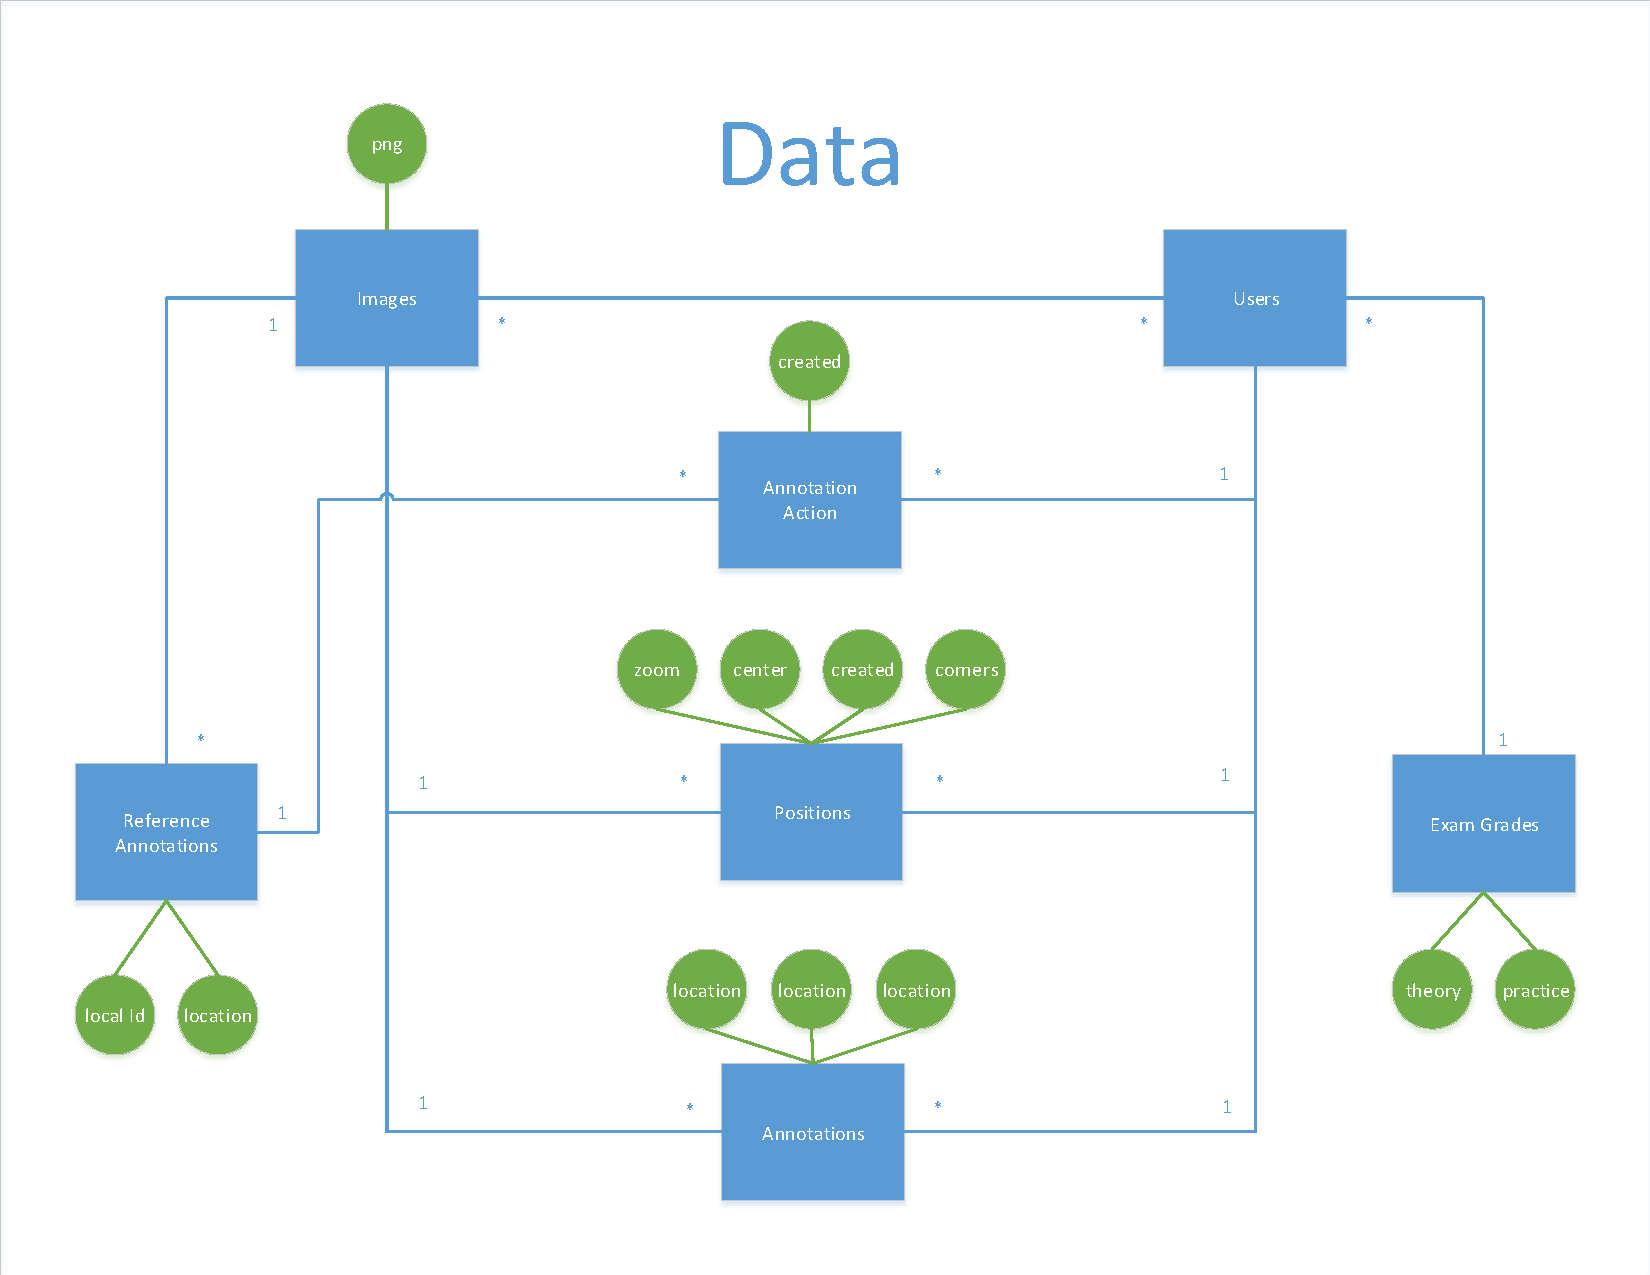
\includegraphics[width=.9\linewidth]{dataDiagram.pdf}
         \caption{Data and their relations}
         \label{fig:data}
       \end{figure}

        
		All this information needs to be downloaded.
		Unfortunately, this can take up to 8 hours using the API while putting stress on the MOOC server.
		After some interruptions to the service, it was decided that the MOOC needed to be installed locally with backups of the original. \newline
        
        For both projects, an excel file containing user information not found on Cytomine was given.
        For the SILVER project, this only included basic information that were irrelevant to the analysis (names, emails, etc..).
        Meanwhile for the GOLD project, the University of Liege students had to partake in multiple graded assignments.
        The excel file given for the GOLD students therefore contained grades for numerous activities.
        These grades will be useful in order to understand some aspects of the user behavior on Cytomine. \newline
        
        
        The project has a dedicated directory to store all this information, usually in a csv format.
        For each data type, image, and user triplet, there is a dedicated file containing this information.
        These files will be opened and read by the Data Manipulation Component for generating statistics and ways to represent data visually.
        
        %todo add image of directory organisation 
        
	\subsubsection{Data Manipulation}
    
    This component is used to interpret the data that's in its most basic form.
    It has multiple outputs based on the parameters set.
    Since it's important to obtain information as a whole on the data set, the component is divided into two main parts:
    \begin{itemize}
        \item[\textbullet] Loading data to Memory: The positions, the annotations, the actions, and the image information data are all loaded to memory.
        \item[\textbullet] Data Handling : Calling numerous methods that extracts important information.
    \end{itemize}

    This component knows and uses the file directory structure.
    This allows it to find the files necessary to do the analysis.
    An object oriented approach was used in order to handle this information.
    In fact, there are multiple classes:

    \begin{itemize}
        \item[\textbullet] Data\_Manager : This class defines an object that will coordinate between the other classes in order to obtain the valuable information necessary.
        \item[\textbullet] Image\_Data : This class defines objects that will contain references to information on a specific image.
        It also comes with operations associated to said image.
        \item[\textbullet] User\_Data : This class defines objects that will contain references to information on a specific user.
        Similarly, to Image\_Data, it comes with numerous operations.
        \item[\textbullet] Module\_Data : This class defines objects that will contain references to information on a specific module.
        Modules are predefined by the teachers as a set of objectives within a certain timeframe.
        There is a subset of images that are associated to a module.
        It therefore contains references to users and images and it also comes with its own operations.
    \end{itemize}

    These instances contain references to richer information.
    This information is handled using dictionaries for fast and easy access.
    For the set of positions associated to a user and image pair, the dictionary contains these key and value pairs:
    \begin{itemize}
        \item[\textbullet] 'x' : Array of X coordinates for all the positions.
        \item[\textbullet] 'y' : Array of Y coordinates for all the positions.
        \item[\textbullet] 'dur': Array of the duration for all the positions.
        \item[\textbullet] 'timestamp': Array of the exact time the positions have been recorded for each position.
        \item[\textbullet] 'zoom' : Array of the zoom values for each position (1 to 10)
        \item[\textbullet] 'corners' : Array containing the four corners for each position.
        The four corners are stored as an array with 4 values.
        These values contain a pair for the X and Y coordinates.
    \end{itemize}

    It is noted that the positions are sorted in regards to the timestamp value.
    This prevents many problems and makes specific operations much easier.
    The dictionary follows a similar structure for annotations that are either associated to an image and user pair (user annotation) or just an image (reference annotation):
    \begin{itemize}
        \item[\textbullet] 'x' : Array of X coordinates for all the annotations.
        \item[\textbullet] 'y' : Array of Y coordinates for all the annotations.
        \item[\textbullet] 'id': Array of the identifiers for all the annotations.
        \item[\textbullet] 'localId': Array of the local identifiers for all the annotations.
        Used for reference annotations.
        This property represents the annotation number shown on the images but also the recommended order of passage for these annotations
        \item[\textbullet] 'type' : Array of the type for all annotations.
        This is either a point or a polygon.
    \end{itemize}

    There are much fewer annotations then there are positions.
    Finally there are also annotation actions for image and user pairs:
    \begin{itemize}
        \item[\textbullet] 'id' : Array of the identifiers of the concerned annotations for all the annotation actions.
        \item[\textbullet] 'action' : Array of the action carried out for all annotation actions.
        The value is always 'select'.
        \item[\textbullet] 'timestamp' Array of the time the annotation action was carried out.
    \end{itemize}
    It is important to know that during the period of January 2017 to September 2017, annotation actions were collected but they did not specify which annotation the action was related to.
    To determine that the component guesses the annotation.
    The component finds the position with the closest timestamp and guesses the annotation closest to that position.
    It's not perfect but it guesses the most likely annotation since at most zooms the user can only see one annotation.\\


    This data is referenced by the proper Image\_Data and User\_Data objects for easy access.
    When loading all this data into memory, extra operations have been carried out.
    The most notable being generating the gaussian surface for each zoom associated to each image.
    This uses a 2 Dimensional Gaussian distribution function.
    The Gaussian plane respects the dimensions of the positions associated to that zoom.
    This allows to better represent a position by not just taking into account the center and corners but the entirety of the field of view of the person.
    The goal is to give more importance to the center pixels of a position over the pixels near the edge.
    This will be very important when deriving statistics generating heatmaps.

    When generating the gaussian with a height of $h$ and a width of $w$.
    The standard deviation set for the height and width are $s_h = \dfrac{h}{6}$ and $s_w = \dfrac{w}{6}$.
    $h_0 = \dfrac{h}{2}$ and $w_0 = \dfrac{w}{2}$ are the center coordinates of the surface.
    $coeff$ is a coefficient based on the zoom.
    The coefficient is a value from 0 to 1, the higher the zoom the higher the coefficient with $coeff = \dfrac{zoom}{max\_zoom}$.
    The equation is :

        \[P(i,j) = \exp(\dfrac{-1}{2}*(\dfrac{(i - h_0)^2}{s_h^2} + \dfrac{(j - w_0)^2}{s_w^2})) * coeff \]

    With $i \in [0, h]$ and $j \in [0, w]$.

    With the standard deviation set, 99 percent of the gaussian distribution is in the surface.
    Therefore when calculating the center point, there is an output close to 1.
    Likewise, when calculating a point near the edge, there is an output close to 0.
    An interesting idea that was not implemented was to was to replace $coeff$ with $\dfrac{1}{2\pi*s_h*s_w}$.
    With that, the integral of all the Gaussian surfaces would be equal to 1.
    The problem with this method is with each zoom level, the height and the width halves in size.
    The surface would be four times as small.
    Therefore, from zoom 1 to 10 there is a factor of $4^{10}$ or about a million.
    The difference in values between zooms would be too extreme.
    This is why a more linear coefficient is used so that Heatmaps are observable.
    In the end, the idea is that the human attention is more focused on the center.
    Therefore a Gaussian distribution is ideal for this particular problem.
    In the following example is shown the Gaussian distribution for a surface with a length and width of 100, and a coefficient of 1. (Figure \ref{fig:gaus22})

    \begin{figure}[H]
      \centering
      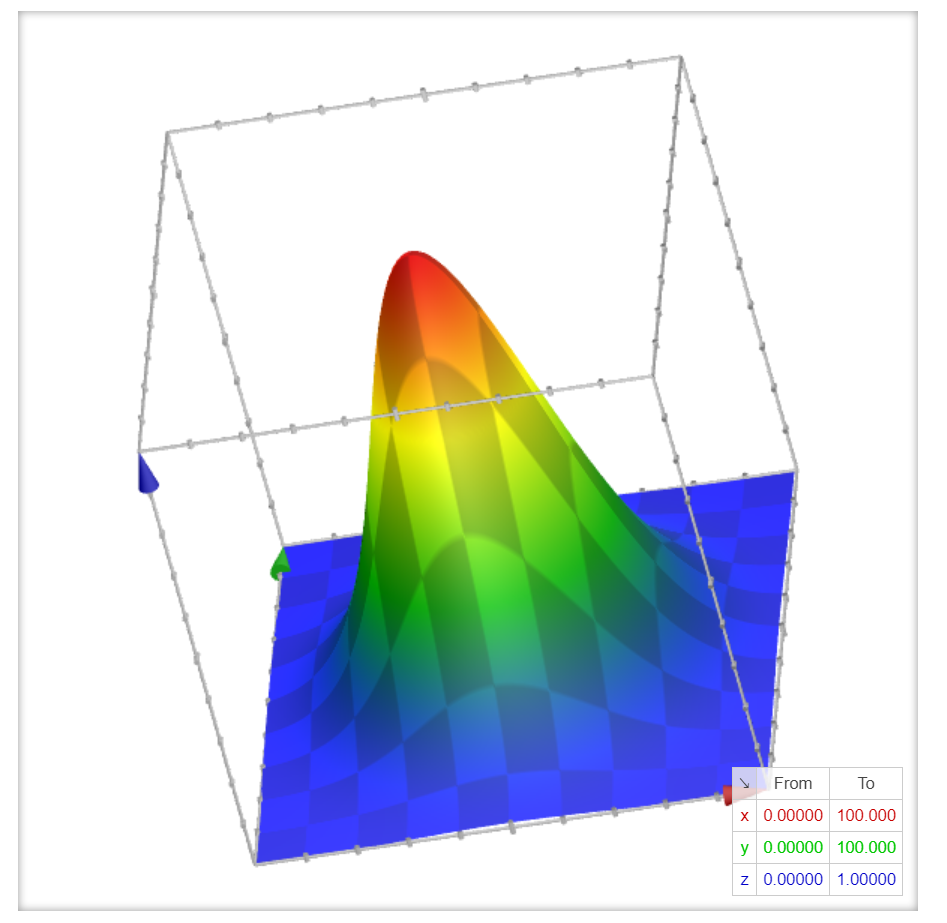
\includegraphics[width=.45\linewidth]{gaussian2D.png}
      \caption{Gaussian Distribution Example}
      \label{fig:gaus22}
    \end{figure}

    Of course, because the work is done on images, there is a limited resolution and the Gaussian is not as smooth.
    This is because each pixel is a point and a point has the value set by the formula.
    \newline

    Once all all this information is stored in memory.
    it is possible to call numerous tasks to analyze the data and draw statistics.
    This includes :

    \begin{itemize}
        \item[\textbullet] Output a Feature File : Students are analyzed individually in regards to the images they visited.
        A set of features is then extracted in regards to their behavior.
        (see \ref{Data_Set} for more information on the contents and structure of the file)
        \item[\textbullet] Output activity over time figures : These figure represents the activity over time of a set of students or simply an individual in regards to different modules.
        It gives a good insight on habits and work consistency of the students.
        These figures depict the number of positions for every single day.
        The weekends are tinted in a light yellow.
        It also shows the activity in regards to the modules.
        Since the modules come with a set schedule, the figure also shows when they start and when they end.
        Finally, the dates for the exams are also a big focus.
        This allows the observation of the students' patterns as a whole or comparing the behavior of particular students.
        An interesting experiment would be to compare the figures for the very best student and the very worst students to get more insight.
        The example in Figure \ref{fig:timelapse} shows the total activity for all the students.
        \item[\textbullet] Output Gaze Map figures : These figures represents the heatmaps of the student activity in regards to an image.
        Since an image is resized to a reasonable resolution, each pixel is assigned a weight based on the user's activity near that pixel.
        Therefore, operations are done pixel by pixel.
        The values assigned rely on the 2D Gaussians generated for the positions.
        The 2D grid for the heatmap was generated with this component but generating and saving the image was implemented by PyGazeAnalyzer.
        Their heatmaps are beautiful but they lack information. For a pixel the color red means that it was the most visited a blue means that it was not a big focus.
        Even with a legend it would be hard to compare different images because the scales would not be the same for many heatmap implementations.
        Depending on the method, generating a heatmap can be a very costly operation.
        Methods include :
        \begin{itemize}
            \item Raw Heatmap : For each position, the respective gaussian values are added into the heatmap at the right position.
            There are some advantages including that it's the fastest and shows clear distinctions between parts of the images.
            Drawbacks include that it is really hard to quantify and compare between users and other images.
            An another issue is with extreme cases the distinctions between regions of the image that been visited are too strong.
            For extreme cases, the most visited region might have such a high heatmap value that the other regions are hard to compare with each other.
            \item Logarithmic Heatmap : The heatmap is generated similarly but a $Log_{10}$ normalizer applied at the end for each pixel.
            The advantages of that is that it's easier to compare areas of an image since the distinctions are smoothed.
            But it's main drawback is that it's really hard to quantify because the normalizer can be too extreme.
            Similarly, it's not straightforward when comparing students and images with each other since the scales are different for each heatmap.
            \item Logarithmic Heatmap Relative to an image : The idea would be to reimplement the previous heatmap for every user of a specific image and standardize the scale.
            Since the minimum heat value will always be 0, this method only looks for the maximum heat value between all the heatmaps for that image.
            This value is set for all the heatmaps and they are drawn. This method's goal was to compare different students for the same image.
            Unfortunately, it still shares most of the same drawbacks of the Logarithmic Heatmap.
            \item Logarithmic Heatmap Relative to a user : This is the same concept as previously but the goal is to compare activity of the same student across multiple images.
            This has the same advantages and drawbacks as the previous heatmap.
            \item Reduced Heatmap : A interesting observation is that it's hard to quantify user observations for long durations.
            The longer a person looks at the same area the less important the positions become over time.
            This explains the attempt to normalize the heatmap using the logarithmic function.
            The problem is that there's no theoretical explanation to why the the logarithmic method should work.
            In this case a pixel is represented by vector instead of a value.
            The vector contains a list of all the respective Gaussian value for each position that is close enough.
            The value is always in the range of $[0,1]$.
            For each pixel, the list is sorted inversely.
            Finally, the value of the pixel is given by a weighted sum of the values of this list.
            The weights follow a geometrical sequence that converges.
            Therefore, after numerous positions, the weights are near 0.
            This normalization method is further explained in the section \ref{enum:score}.
            In this case, $w$ is set to 0.95 and the sequence converges at a value of 20.
            Therefore, the heat values from each pixel belong in the range $[0,20]$.
            The maximum value for all heatmaps can easily be set to 20.
            This method has a more relaxed normalization and it is much easier to compare different heatmaps and infer heat values by looking at the image.
            The main drawback is that it's much slower.
            Since for each pixel, the algorithm is given a list to sort a values to weight it takes much more time.
        \end{itemize}
        %% todo : images of different heatmaps.
        \item[\textbullet] Output Scan Path Figures : These figures represents the path taken by the students when they scan through an image.
        Another Idea that seems interesting is to observe a student's viewing order when looking at images.
        The idea is to draw arrow an plot that connects each position to the following position.
        After doing so for all the positions, it's possible to analyze the viewing order.
        Unfortunately, in most cases there are too many positions.
        This is why clustering is used to group up close positions in regards to time and space.
        K-Means clustering was implemented with K predetermined and ranging from 10 to 50.
        With this amount of clusters there may be a small loss in information but it allows the Scan Path to be observable.
        These clusters are arranged by the average time of their positions.
        Each cluster is also given a weight based on the number of positions that belong to it.
        This makes the scan path complete in a sense that it shows most of the needed information relating to the user's viewing order.
    \end{itemize}
    %todo add image examples
    \begin{figure}[H]
      \centering
      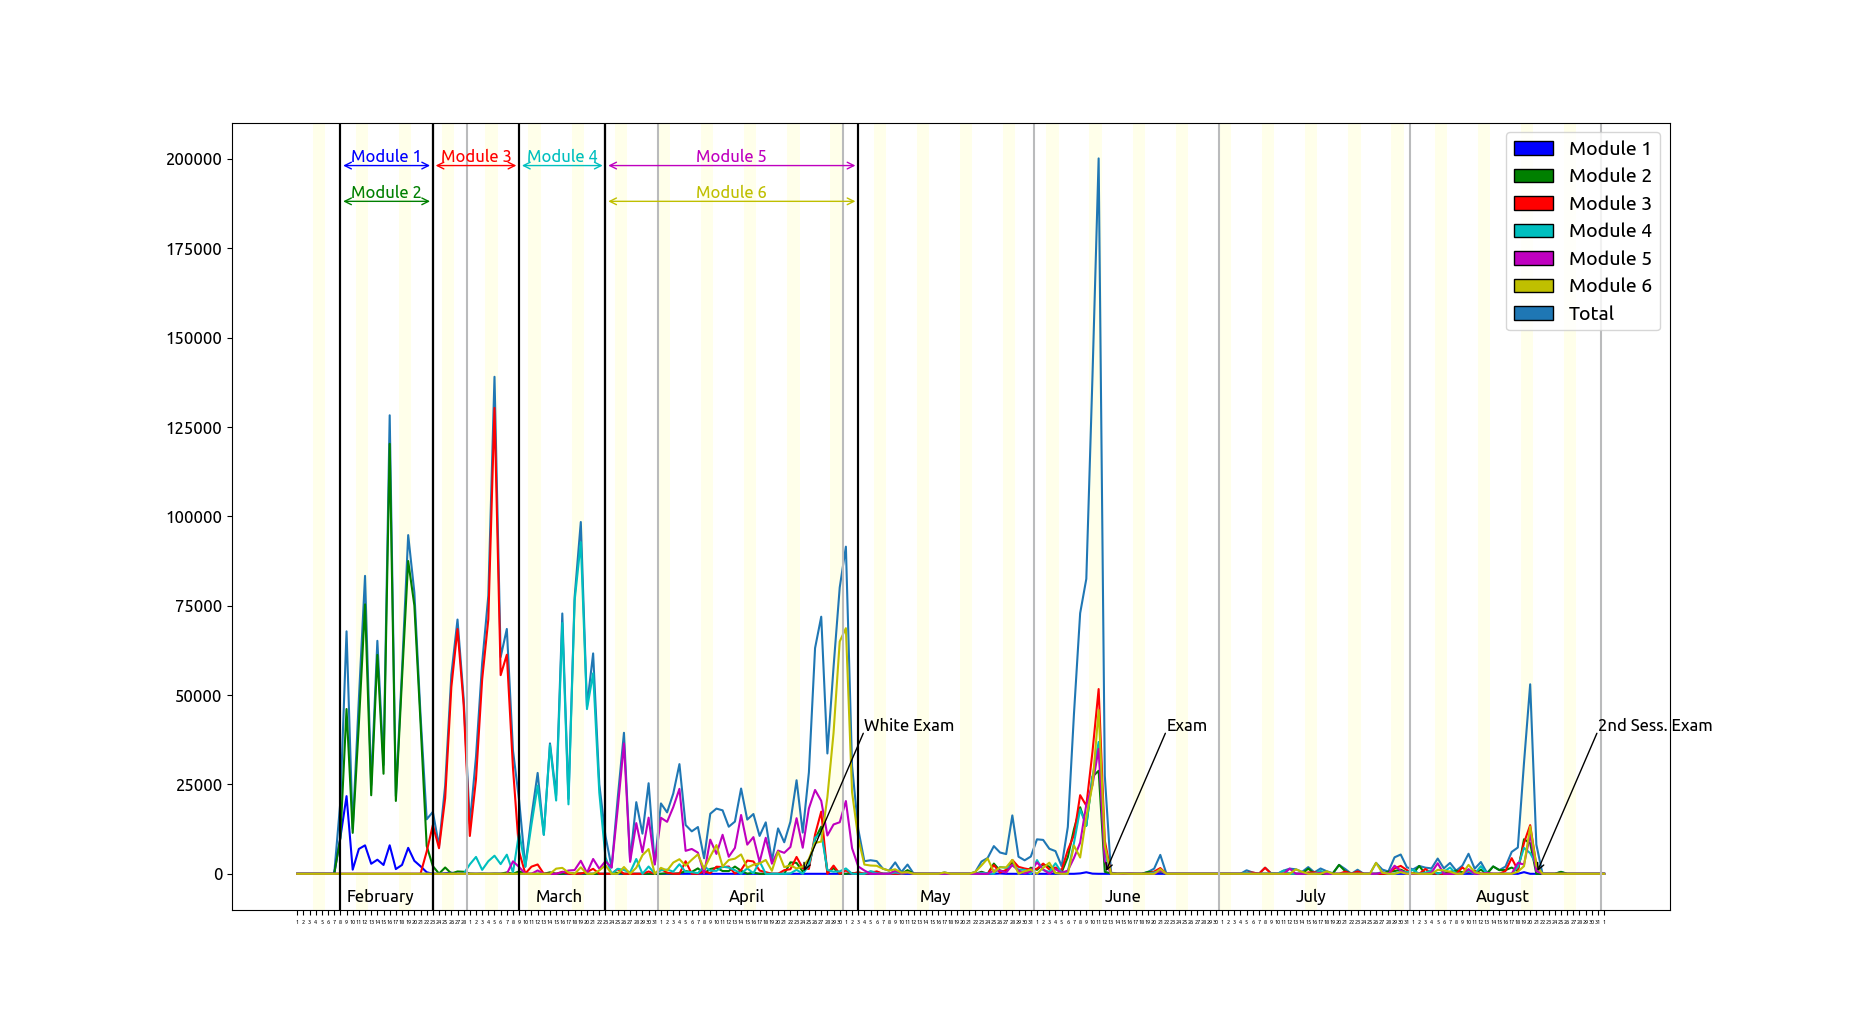
\includegraphics[width=.9\linewidth]{timelapse.png}
      \caption{Overall Student Activity over Time}
      \label{fig:timelapse}
    \end{figure}


    \subsubsection{Data Learning}


\section{Data Analysis}

	\subsection{Experiments}
    
    
    Even though the data was obtained for both the GOLD and SILVER projects, the experiments were on run on the GOLD project.
    This is due to the many constraints given by the SILVER project including the sample size and the lack of results (student grades).
    The goal for most experiments is to learn a specific grade the student obtained based on all the information gathered in the Data Manipulation component.
    There were over 2000 features generated, where each one can weigh in on the prediction.
    These features were used to learn over 13 grades including the final grade obtained by these students (first session).\newline
    
    
    Due to the nature of the dataset, regression trees were the most ideal.
    The somewhat small dataset paired with a large amount of features is a big constraint to work with.
    Therefore, Ensemble methods were used and tested.
    This includes Random Forest regression and Extra Trees regression using sklearn.\newline
    
    The Learning component is given a statistics file containing rows of students paired with their features.
    The features are split into three categories :
    \begin{itemize}
\item[\textbullet] \textbf{M} : Meta-data variables, these variables have no statistical significance.
These variables usually contain basic information on the users.\\
\item[\textbullet] \textbf{X} : Variables with statistical significance, these variables mostly include data extracted from the Cytomine website.
Either individual image variables or variables on the set of images.
These variables are used in the machine learning model as input variables.\\
\item[\textbullet] \textbf{Y} : Result variables, these variables is what the algorithm is attempting to guess using the  \textbf{X} variables.
These variables are used in the machine learning model as output variables.\\
\end{itemize}
    
    
    
    \subsection{Data Set} \label{Data_Set}
    
    	\subsubsection{Students}
    Like mentioned earlier, there are a total of 395 students in the data set.
    Students are defined by their features and the grades obtained.
    These student followed the course HISL054, "General histology and alternative experimentation methods that do not use animals" at the University of Liege during the academic year 2016-2017.
    Most of the work done by the students is done online using the MOOC and Ecampus.
    Ecampus is a website used by students and teachers of the University of Liege to exchange information used for courses.
    In fact all of the assignments for this course are explained on Ecampus.
    The issue with this is that it's a different entity from the MOOC and therefore is not ideal for fetching information.
    But it's not much of a problem because there's nothing to retrieve about students on Ecampus that is not already known.\newline
    
    When applying machine learning techniques, students with a 0/20 were taken out of the sample.
    This is due to the fact those students defaulted to signing the exam.
    Since there are too few that do so, there's not enough information to find correlations between people who sign and the features.
    Keeping students who sign also increases the error rate because they are extreme cases.
    The goal is to guess how well the exam would have went for the students.
    If the student decides not to bother with taking the exam, it's a lost sample.\newline
    
    	\subsubsection{Teacher Input : Grades}
    
    %% QROL - Question a Reponse Ouverte Longue
    %% QCM - Question a choix multiples
    %% QCL - incidence de coupe et identification
    
	The students are evaluated by multiple exams and quizzes, these take the form of:
    \begin{itemize}
    \item[\textbullet]  QCM : Multiple choice question test.
    Students are given questions and have to respond with 1 out of the 9 (or less) options.
    They have to set a degree of certainty for each response.
    The exam results are then calculated by a machine.
    The students are also given more boxes to answer in case they make a mistake the first time.(Figure \ref{fig:qcm})
    \begin{figure}[H]
    \centering
     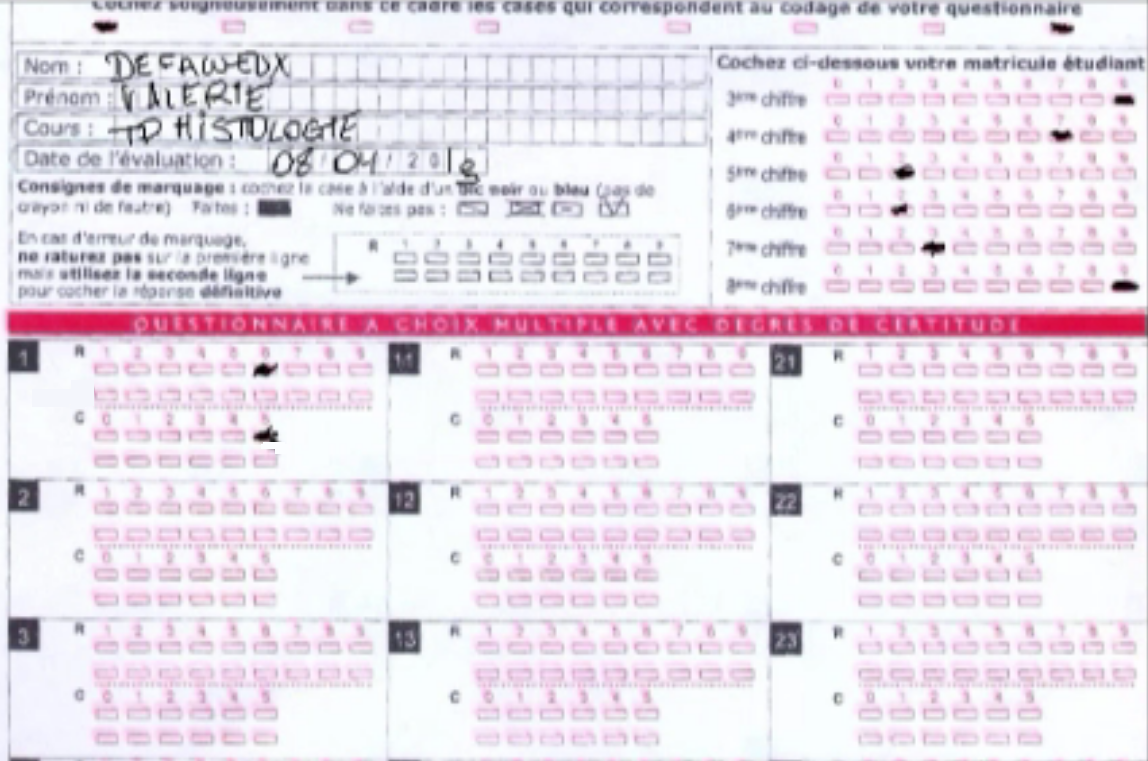
\includegraphics[width=0.4\linewidth]{exam_qcm.png}
     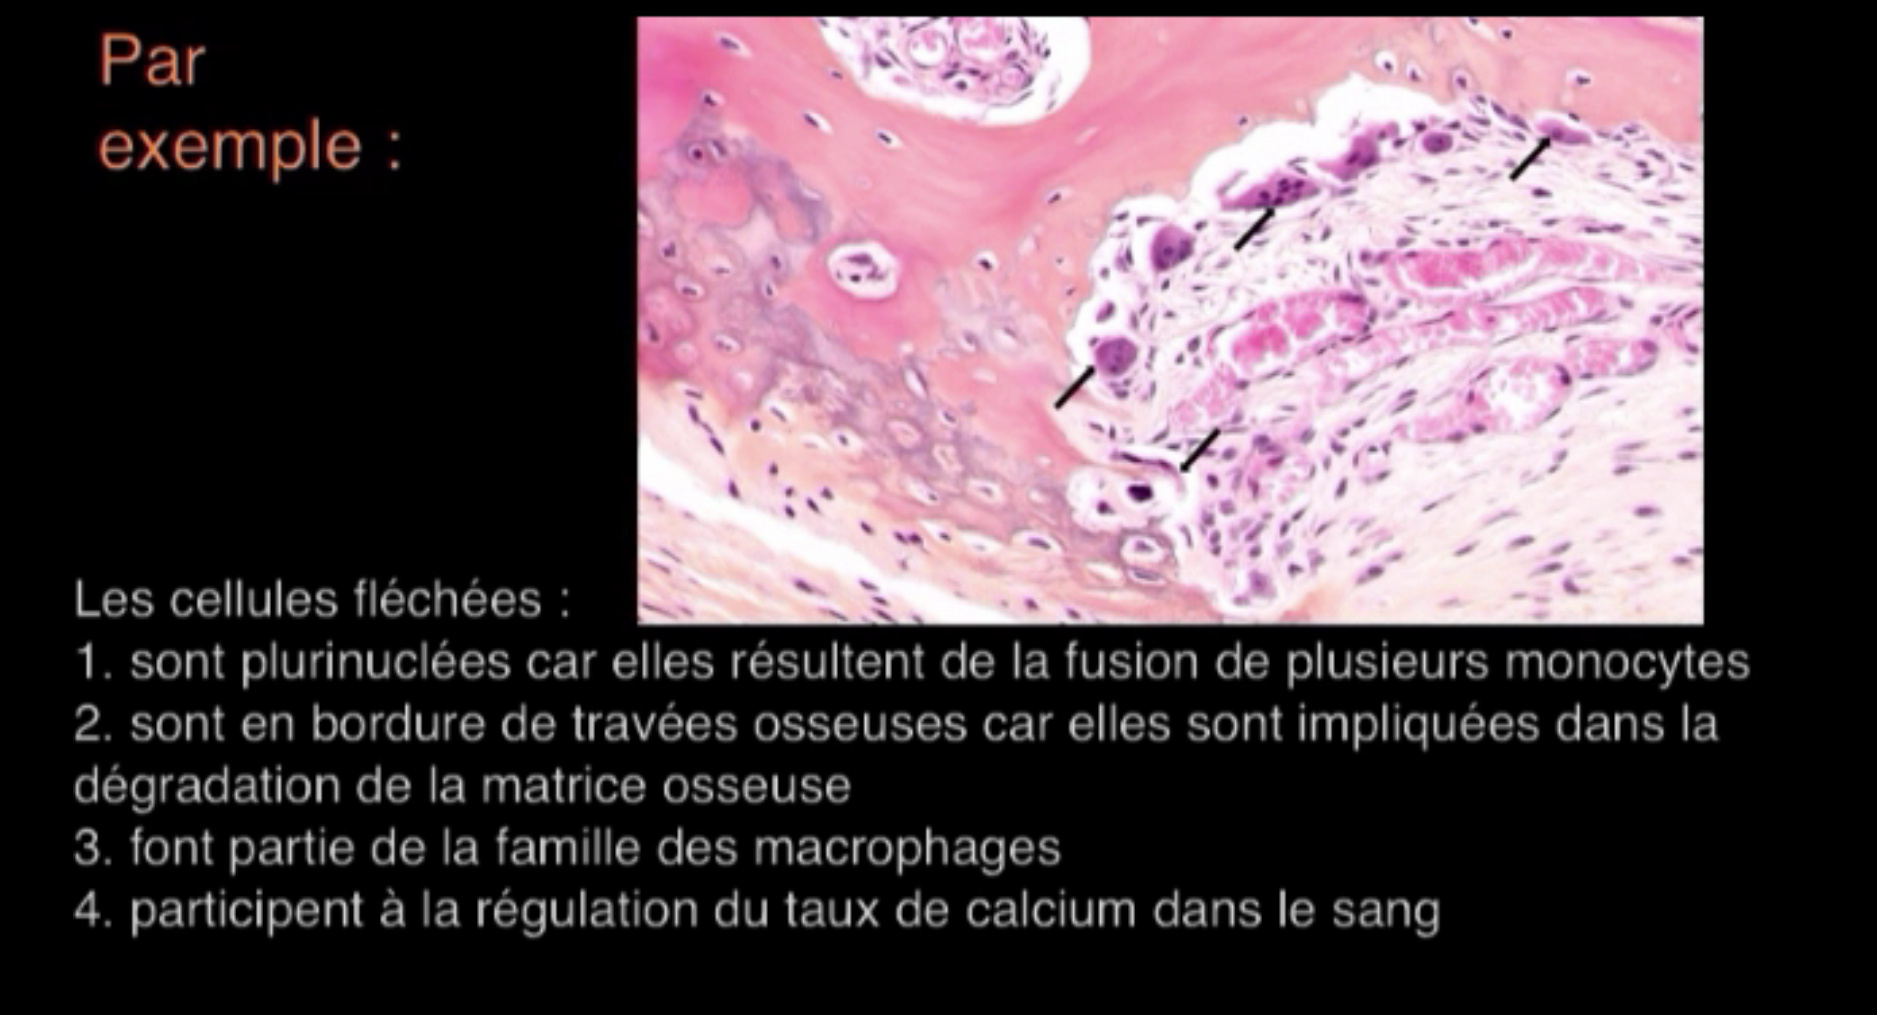
\includegraphics[width=0.5\linewidth]{exam_qcm2.png}
     \caption{QCM sheet and question example}
     \label{fig:qcm}
    \end{figure}
	\item[\textbullet]  QCL : Identification and Incidence test.
	Graded similarly to a QCM, the students are given multiple questions to answer and they have to fill out a form.
	The are a couple differences.
	Each question is split into two, the identification and the incidence.
	For the identification, the students have to identify an object on an image.
	They are given an exhaustive list of possible answers ranging from cells to tissues.
	Each answer contains is associated to a 3 digit code that they need to write on the form.
	For the incidence, the students needs to identify how the observed object "was cut".
	There are a total of 3 possible answers, transversal, longitudinal, and undetermined.
	The answer is written on the form under the identification answer.(Figure \ref{fig:qcl})
      \begin{figure}[H]
    \centering
     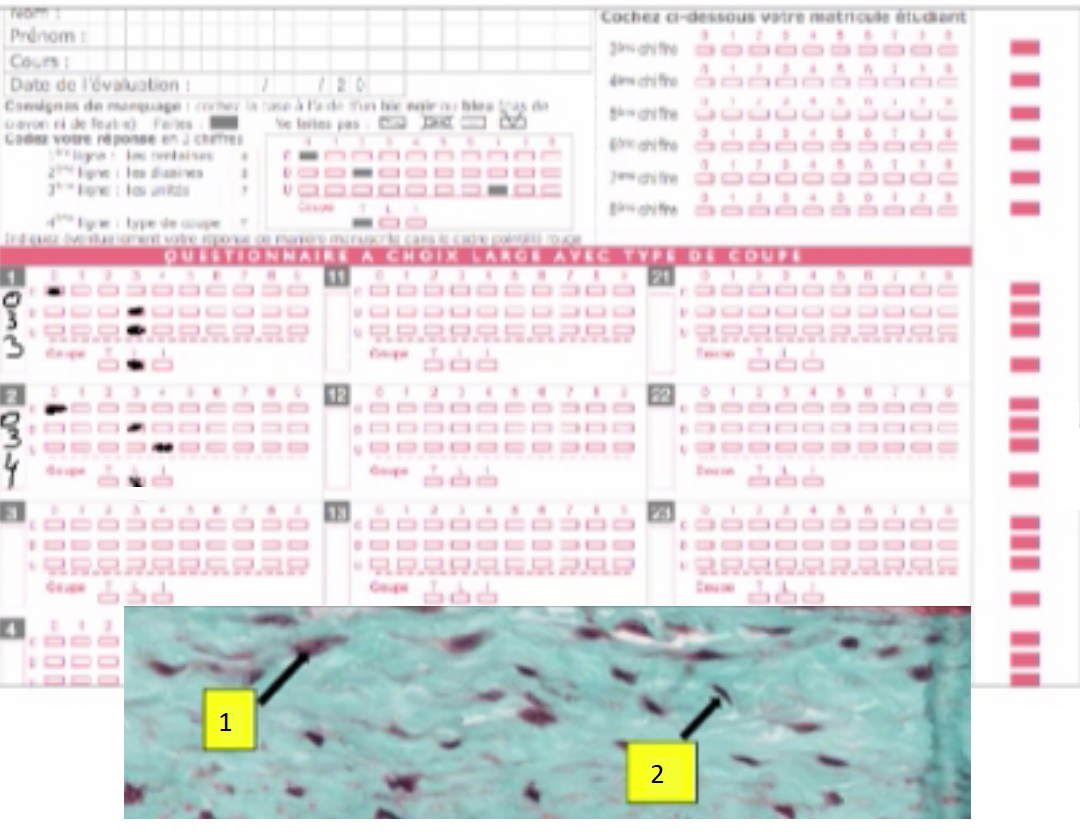
\includegraphics[width=0.42\linewidth]{exam_qcl2.png}
     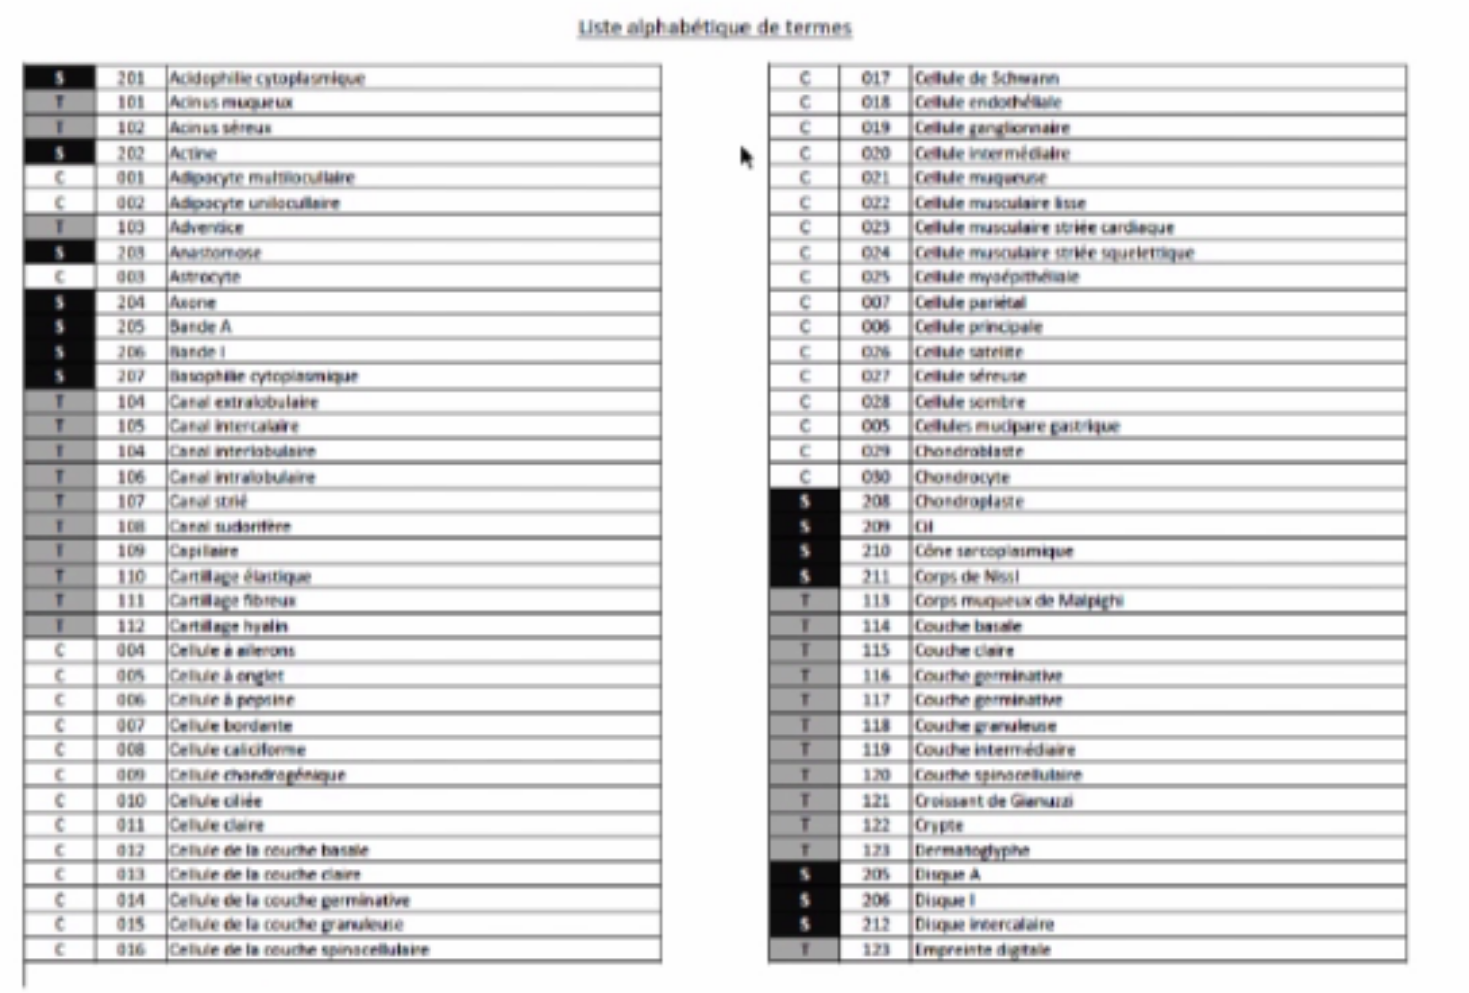
\includegraphics[width=0.5\linewidth]{exam_qcl.png}
     \caption{QCL sheet with question example and list of answers}
     \label{fig:qcl}
    \end{figure}
	\item[\textbullet]  QROL : Long answer open question test.
	Students are to write and explain their answers in a detailed fashion. (Figure \ref{fig:qrol})
          \begin{figure}[H]
    \centering
     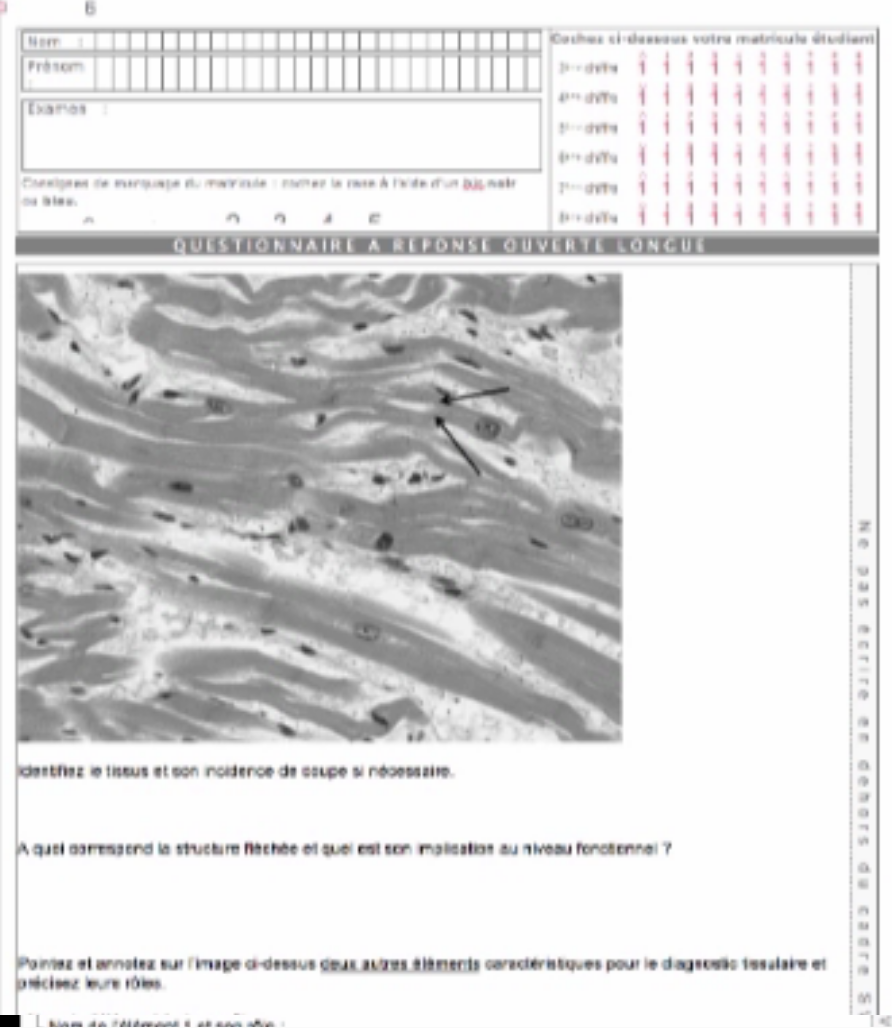
\includegraphics[width=0.45\linewidth]{exam_qrol.png}
     \caption{QROL sheet with a set of questions}
     \label{fig:qrol}
    \end{figure}
    \end{itemize}
    
    These variables will be denoted as \textbf{Y} variables for output.
    Out of the 13 results associated to the students, 3 were white tests given as a practice tool : 
    \begin{itemize}
    \item[\textbullet]  QCL identification white test.
	\item[\textbullet]  QCL incidence white test.
	\item[\textbullet]  Practical QCM white test.
    \end{itemize}
    Similarly, 7 graded exams and quizzes were given to students with 3 being theoretical and 4 being practical.
    Something to note for the practical exam is that there are 2 different exam forms for the QCM and the QRL. This means that half the students are given different questions from the other half.
    The list of exams include:
    \begin{itemize}
    \item[\textbullet]  QROL1 theory (10\%).
    \item[\textbullet]  QROL2 theory (10\%).
    \item[\textbullet]  QCM theory (30\%).
    \item[\textbullet]  QCM practical (20\%).
    \item[\textbullet]  QROL practical (10\%).
    \item[\textbullet]  QCL identification Practical (16\%).
    \item[\textbullet]  QCL incidence Practical (4\%).
    \end{itemize}
    Finally, based on the previous results given, there are:
    \begin{itemize}
    \item[\textbullet] Total Theory (50\%)
    \item[\textbullet] Total Practical (50\%)
    \item[\textbullet] global Grade (100\%)
    \end{itemize}
    
    Most of the experiments are done using one of these grades as Y variables.
    In later experiments, some variables will be set as features.
    The learning of final grades using white test results as bonus features (\textbf{X} variable) could yield better results.
    Learning theoretical grades while also using practical grades and vice versa can also give some interesting results. \\

    Statistics can be derived for each variable :\\

    \begin{center}
      \begin{tabular}{| p{1cm} | p{0.6cm} | p{0.6cm} | p{0.6cm} | p{0.6cm} | p{0.6cm} | p{0.6cm} | p{0.6cm} | p{0.6cm} | p{0.6cm} | p{0.6cm} | p{0.6cm} | p{0.6cm} | p{0.6cm} | }
      \hline
      & \tiny{White Test QCL ID} & \tiny{White Test QCL IC} & \tiny{White Test QCM} & \tiny{QROL Theory 1} & \tiny{QROL Theory 2} & \tiny{QCM Theory} & \tiny{QCM Practical} & \tiny{QROL Practical} & \tiny{QCL ID Practical} & \tiny{QCM IC Practical} & \tiny{Total Theory} & \tiny{Total Practical} & \tiny{Global Grade}\\ \hline
      \tiny{Minimum} & \tiny{1.33} & \tiny{1.33} & \tiny{0.36} & \tiny{0.44} & \tiny{0.67} & \tiny{3.43} & \tiny{3.16} & \tiny{0.29} & \tiny{1} & \tiny{2} & \tiny{2.59} & \tiny{2.01} & \tiny{1.68}\\ \hline
      \tiny{Maximum} & \tiny{18.67} & \tiny{20} & \tiny{19.64} & \tiny{20} & \tiny{20} & \tiny{17} & \tiny{17.32} & \tiny{18.82} & \tiny{20} & \tiny{20} & \tiny{17.8} & \tiny{17.99} & \tiny{17.85}\\ \hline
      \tiny{Average} & \tiny{8.09} & \tiny{12.17} & \tiny{10.18} & \tiny{10.67} & \tiny{12.16} & \tiny{10.05} & \tiny{10.88} & \tiny{8.6} & \tiny{11.15} & \tiny{15.03} & \tiny{10.56} & \tiny{10.81} & \tiny{10.63}\\ \hline
      \tiny{Median} & \tiny{8} & \tiny{13.33} & \tiny{10.31} & \tiny{10.75} & \tiny{12.83} & \tiny{10.03} & \tiny{10.8} & \tiny{7.93} & \tiny{11} & \tiny{15} & \tiny{10.75} & \tiny{10.76} & \tiny{10.67}\\ \hline
      \tiny{Variance} & \tiny{14.09} & \tiny{17.67} & \tiny{13.3} & \tiny{16.78} & \tiny{19.51} & \tiny{6.41} & \tiny{7.93} & \tiny{18.92} & \tiny{16.48} & \tiny{9.35} & \tiny{8.46} & \tiny{9.92} & \tiny{8.64}\\ \hline
      \tiny{Standard Deviation} & \tiny{3.75} & \tiny{4.2} & \tiny{3.36} & \tiny{4.09} & \tiny{4.41} & \tiny{2.53} & \tiny{2.81} & \tiny{4.34} & \tiny{4.06} & \tiny{3.05} & \tiny{2.9} & \tiny{3.15} & \tiny{2.94}\\ \hline
      \end{tabular}


    \end{center}


    Teachers also input basic student information, but it mostly consists of general information that won't be used in the experiments.
    These will be denoted as \textbf{M} variables:
   	\begin{itemize}
   	\item[\textbullet] ID Cytomine : The Cytomine ID associated to the user. (Compulsory)
    \item[\textbullet] LAST NAME : User's last name.
    \item[\textbullet] FIRST NAME : User's First name (forename).
    \item[\textbullet] GROUP : group user belongs in (GOLDULiege, GOLD, or SILVER).
    GOLDULIEGE is a subset of GOLD containing the set of students following the course.
    This will be used for the analysis.
    \item[\textbullet] USERNAME CYTOMINE : user's Cytomine username.
   	\end{itemize}
    
    
    \subsubsection{Features pre-Calculated}
    
    There are over two thousand features calculated and generated by the Data Manipulation component.
    These variables belong to the \textbf{X} category and are listed:
   
   \begin{itemize}
    \item[\textbullet] NB IMAGES VISITED : The total number of different images that a user has opened over the course of the year.\\
    \item[\textbullet] TOTAL NB POSITIONS : The total number of positions obtained from all the images opened.\\
    \item[\textbullet] AVG NB POSITIONS : The mean number of positions obtained relative to all the images opened.\\
    
    \item[\textbullet] MEDIAN NB POSITIONS : The median number of positions  obtained relative to all the images opened.\\
    \item[\textbullet] TOTAL IMAGE VIEWING TIME (s) : Total amount of time spent viewing images.\\

    \item[\textbullet] AVG IMAGE VIEWING TIME (s) : Mean amount of time spent viewing images.\\

    \item[\textbullet] MEDIAN IMAGE VIEWING TIME (S) : Median amount of time spent viewing images.\\

    \item[\textbullet] NB POSITIONS AT ZOOM <x> : with <x> between 1 and 10, represents the zoom level of a position.
    1 variable per zoom value.
    It represents the total number of positions at zoom <x>.\\
    \item[\textbullet] AVG ZOOM : The mean zoom level over all the positions collected.\\
    \item[\textbullet] MEDIAN ZOOM : The median zoom level over all the positions collected.\\
    \item[\textbullet] TOTAL NB ANNOTATION ACTIONS : The total number of times the user clicked on a reference annotation.\\
    \item[\textbullet] AVG NB ANNOTATION ACTIONS : The mean number of times the user clicked on a reference annotation.\\
    \item[\textbullet] MEDIAN NB ANNOTATION ACTIONS : The median number of times the user clicked on a reference annotation.\\
    
    \item[\textbullet] AVG NB POSITIONS AT ZOOM <x> : with <x> between 1 and 10, represents the zoom level of a position.
    1 variable per zoom value.
    It represents the mean number of positions at zoom <x> relative to all images visited.\\
    \item[\textbullet] MEDIAN POSITIONS AT ZOOM <x> : with <x> between 1 and 10, represents the zoom level of a position.
    1 variable per zoom value.
    It represents the median number of positions at zoom <x> relative to all images visited.\\
    %% TODO : Picture of a gaussian at highest zoom
    \item[\textbullet] \label{enum:score} SCORE OF ANNOTATION <y> AT IMAGE <x> : with <y> being the annotation identifier and <x> being the image identifier.
    When images have annotations, students tend to focus on these points.
    For each position, the program generates a 2 Dimensional Gaussian function to represent the position.
    The size and values of this Gaussian relies on the zoom of the position.
    For example at the center of the Gaussian with the highest zoom, the value is 1.
    While at the lowest zoom the value is $1/MAX\_ZOOM$.
    \begin{figure}[H]
\begin{center}
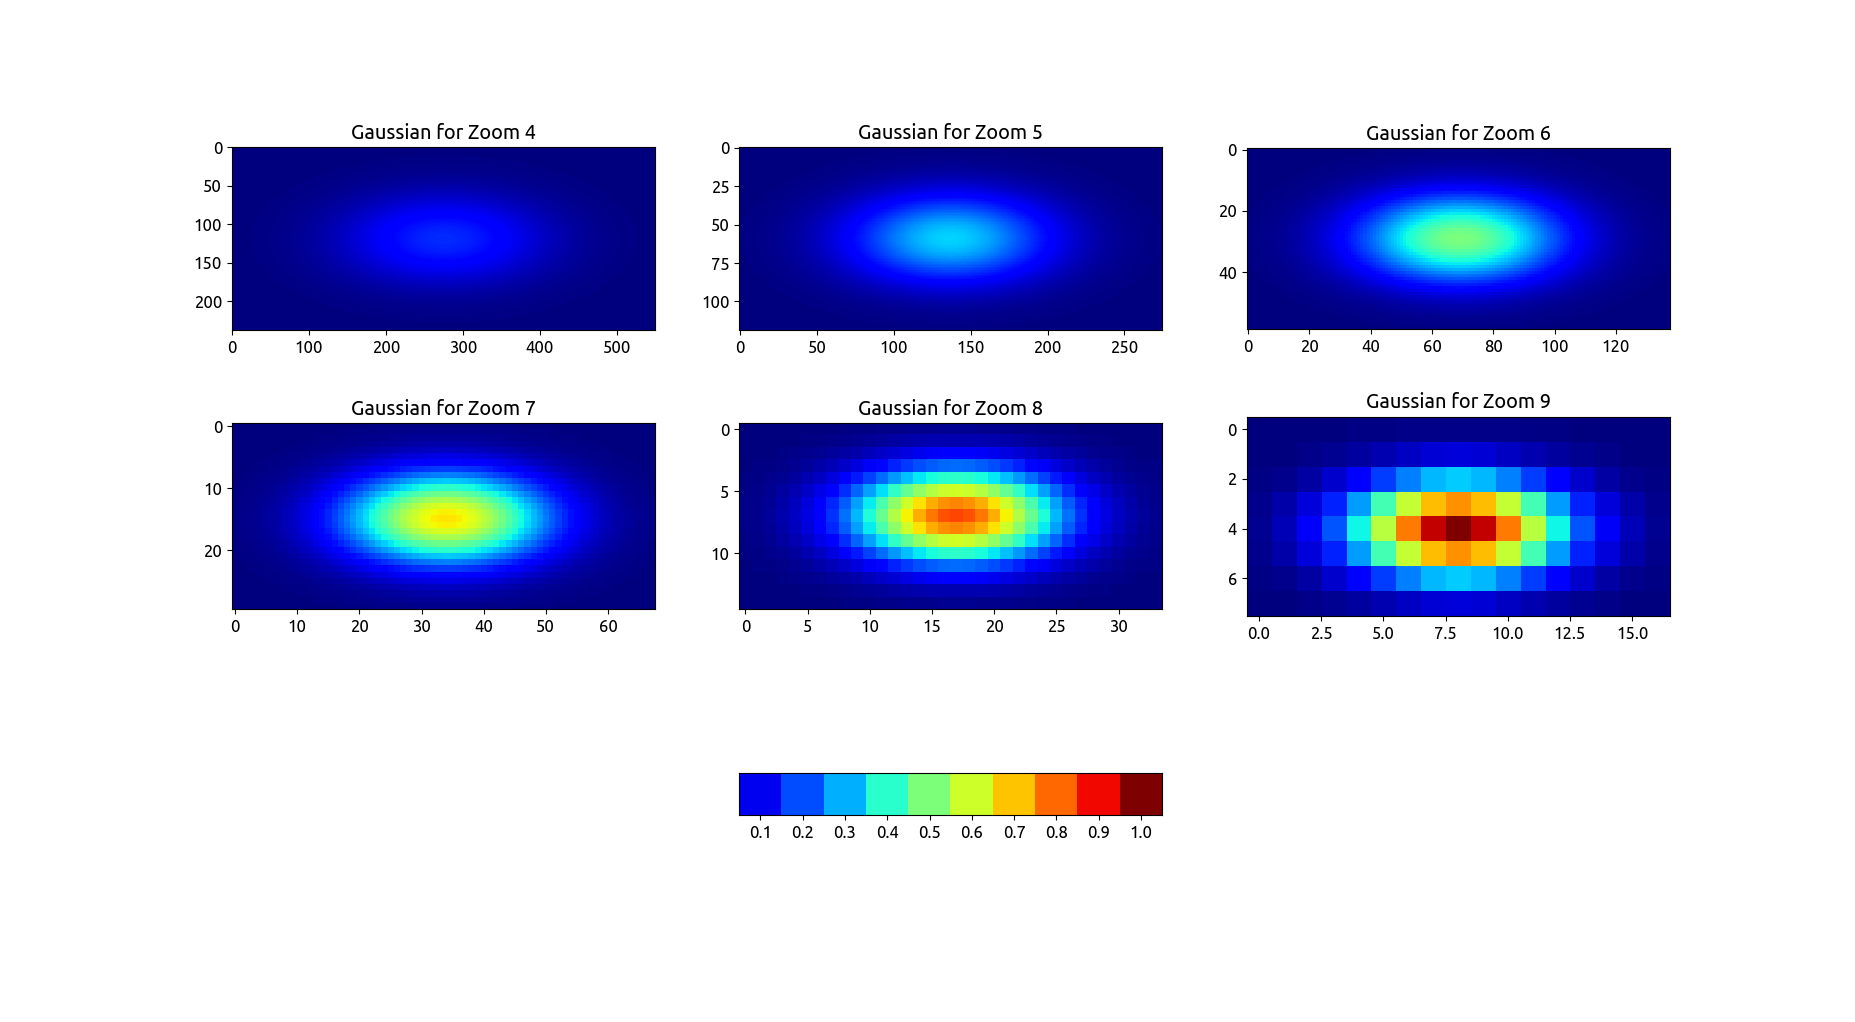
\includegraphics[scale=0.35]{gaussian.png}
\caption{Example Gaussian Grids for an Image that has a zoom up to 9}
\end{center}
\end{figure} 
   
   So each annotation has a center coordinate.
   For this coordinate, a list of Gaussian values is generated based on all the positions near the annotation.
   This vector is sorted inversely.
   It's important to note that it does not take much time for the student to assimilate all the information on a part of an image.
   So the idea is to weight these positions to the point that after enough positions, the next ones would have a weight of close to 0.
To do so, a geometrical sequence was used:  
	\[\sum\limits_{i=0}^N w^i\]

N is the number of positions.
In our case, $w$ was set as 0.95.
This means that this sequence converges to 20, and after about 50 positions the sequence is close to the convergence value (about 18).
Since the list of Gaussian values are sorted, the highest values will have the highest weight.
The equation becomes :
	\[score = \sum\limits_{i=0}^N L[i]*w^i\]
With L being the list of Gaussian values for the annotation.
This means that the highest value has a weight of 1, the second a weight of 0.95, the third $0.95*0.95$, and so on.
The value calculated is then used for the score.
If a student actually observed in detail the annotation, they would usually get values above 10.\\

    \item[\textbullet] USER SCORE AT IMAGE <x> : With <x> the image identifier on Cytomine.
    The users are given scores between 0 and 1 (not opening an image gives the user a score of 0).
    The score represents how well the user observed the annotations in the given image.
    In short, if a user spends a good amount of time on top of an annotation or if the user clicks on the annotation, he/she will get points for that annotation.
    Doing so for all annotations gives a final score.
    The score for an annotation is given by the previous variable (SCORE OF ANNOTATION <y> AT IMAGE <x>) and re dimensioned so this variable returns a score between 0 and 1.
    If the image does not have any annotation, the scores for are calculated for the entire image and the average is returned. \\
    
    \item[\textbullet] AVERAGE USER SCORE : The average of all the scores defined previously for a user. \\
    
    \item[\textbullet] NB POSITIONS AT IMAGE <x> : with <x> being the image Identifier, represents the number of positions recorded at that image for a user. \\
    
   \item[\textbullet] TIME SPENT AT IMAGE <x> : With <x> being the image identifier, represents the total time spent on an image for a user. \\
   
   \item[\textbullet] NB OF ANNOTATION ACTIONS AT IMAGE <x> : With <x> being the image identifier, represents the number of annotation Actions at that image for a user. \\
      
    \item[\textbullet] NB OF POSITIONS WITH ZOOM <y> AT IMAGE <x> : With <x> being the image identifier and <y> being the zoom value [1-10].
    It Represents the number of positions for a certain zoom  at that image for a user. \\

    \item[\textbullet] NB IMAGES VISITED DURING MODULE <x>: The total number of different images that a user has opened that are associated to the module <x>.\\
    
    \item[\textbullet] AVG NB POSITIONS DURING MODULE <x>: The mean number of positions obtained relative to all the images opened that are associated to the module <x> during the corresponding time period.\\
    
    \item[\textbullet] MEDIAN NB POSITIONS DURING MODULE <x>: The median number of positions obtained relative to all the images opened that are associated to the module <x> during the corresponding time period.\\
    
    \item[\textbullet] TOTAL NB POSITIONS DURING MODULE <x>: The total number of positions obtained from all the images associated to the module <x> during the corresponding time period.\\
    
    \item[\textbullet] TOTAL TIME SPENT DURING MODULE <x> (s) : Total amount of time spent viewing images associated to the module <x> during its given time period.\\    
    
    \item[\textbullet] AVG TIME SPENT DURING MODULE <x> (s) : Mean amount of time spent viewing images associated to the module <x> during its given time period.\\    
    
    \item[\textbullet] MEDIAN TIME SPENT DURING MODULE <x> (s) : median amount of time spent viewing images associated to the module <x> during its given time period.\\
    
    \item[\textbullet] NB POSITIONS DURING MODULE <y> FOR IMAGE <x> : with <x> being the image Identifier of an image associated to the module <y>.
    This represents the number of positions recorded at that image for a user during the module's time period. \\
       
    \item[\textbullet] TIME SPENT DURING MODULE <y> FOR IMAGE <x> : with <x> being the image Identifier of an image associated to the module <y>.
    This represents the time spent at that image for a user during the module's time period. \\
    
    \item[\textbullet] NB ANNOTATION ACTIONS DURING MODULE <y> FOR IMAGE <x> : with <x> being the image Identifier of an image associated to the module <y>.
    This represents the number of annotation actions recorded at that image for a user during the module's time period. \\
     
     
     \item[\textbullet] NB POSITIONS WITH ZOOM <z> DURING MODULE <y> AT IMAGE <x> : with <x> being the image Identifier of an image associated to the module <y>.
     This represents the number of positions recorded at that image for a user during the module's time period with zoom <z>.
     The zoom value <z> ranges from 1 to 10. \\
     
     \item[\textbullet] AVERAGE ZOOM DURING MODULE <y> FOR IMAGE <x> : with <x> being the image Identifier of an image associated to the module <y>.
     This represents the average zoom level of all the positions recorded at that image for a user during the module's time period. \\
     
     \item[\textbullet] MEDIAN ZOOM DURING MODULE <y> FOR IMAGE <x> : with <x> being the image Identifier of an image associated to the module <y>.
     This represents the median zoom level of all the positions recorded at that image for a user during the module's time period. \\
     
     \item[\textbullet] NB POSITIONS AT ZOOM <z> DURING MODULE <x> : with <z> between 1 and 10, calculated for all the images associated to the module <x>.
     This represents the number of positions for a specific zoom for a user during the module's time period. \\
     
	\item[\textbullet] AVERAGE NB POSITIONS AT ZOOM <z> DURING MODULE <x> : with <z> between 1 and 10, calculated for all the images associated to the module <x>.
	This represents the mean number of positions for a specific zoom for a user during the module's time period. \\

	\item[\textbullet] MEDIAN NB POSITIONS AT ZOOM <z> DURING MODULE <x> : with <z> between 1 and 10, calculated for all the images associated to the module <x>.
	This represents the median number of positions for a specific zoom for
a user during the module's time period. \\ 
	
	\item[\textbullet] TOTAL NB ANNOTATION ACTIONS DURING MODULE <x> : With <x> being the module identifier, it represents the total number of annotation  actions for a user during the module's time period. \\ 
	
	\item[\textbullet] AVG NB ANNOTATION ACTIONS DURING MODULE <x> : With <x> being the module identifier, it represents the mean number of annotation  actions for a user during the module's time period. \\ 
		
	\item[\textbullet] MEDIAN NB ANNOTATION ACTIONS DURING MODULE <x> : With <x> being the module identifier, it represents the median number of annotation  actions for a user during the module's time period. \\ 

	\item[\textbullet] AVERAGE USER SCORE DURING MODULE <x> : With <x> being the module identifier, it represents the average predefined score for a user for the module's images during the respective time period. \\ 
    
	\item[\textbullet] USER SCORE AT IMAGE <y> DURING MODULE <x> : With <x> being the module identifier and <y> the image identifier, it represents the predefined score at the image for a user during the module's time period. \\     
	
	\item[\textbullet] SCORE OF ANNOTATION <z> AT IMAGE <y> DURING MODULE <x> : With <x> being the module identifier and <y> the image identifier, it represents the predefined score of the annotation <z> at the image for a user during the module's time period. \\     
         
    \item[\textbullet] PERCENT TIME WORKED AT NIGHT : Value from 0 to 1.
    This represents the ratio of the time spent working from 6pm to 6am.
    
    \item[\textbullet] PERCENT TIME WORKED LATE : Value from 0 to 1.
    This represents the ratio of the time spent working from 1am to 6am.
        
    \item[\textbullet] PERCENT TIME WORKED MORNING : Value from 0 to 1.
    This represents the ratio of the time spent working from 6am to 12pm.
    
    \item[\textbullet] NUMBER OF DAYS WORKED : The total number of days where a user opened at least one image.
    
    \item[\textbullet] PERCENT TIME WORKED DURING MODULE <x> : When working on Cytomine, the user can open images associated during a module during its time period or outside of it.
    This represents the ratio of the user activity during the time period.
    
	\item[\textbullet] ANNOTATION <y> VISITED BEFORE ANNOTATION <y + 1> AT IMAGE <X> : This binary variable determines whether or not a student visited the annotation <y> before the annotation <y + 1> for an image <x>.
	The users are encouraged to study the reference annotation in a specific order.
    
    \end{itemize}
    

    %% todo add conclusion
    
    \subsection{Results}

    \subsubsection{Comparing Timelines}

        In this small experiment, there were a total of 8 timelines geneated.
        Four of those belonging to the students with the highest grades and four belonging to the students with the lowest grades.
        The simple objective is to compare the results from the two sets and also compare results within a set. (Figures \ref{fig:tm1} and \ref{fig:tm2})

      \begin{figure}[H]
      \centering
  	  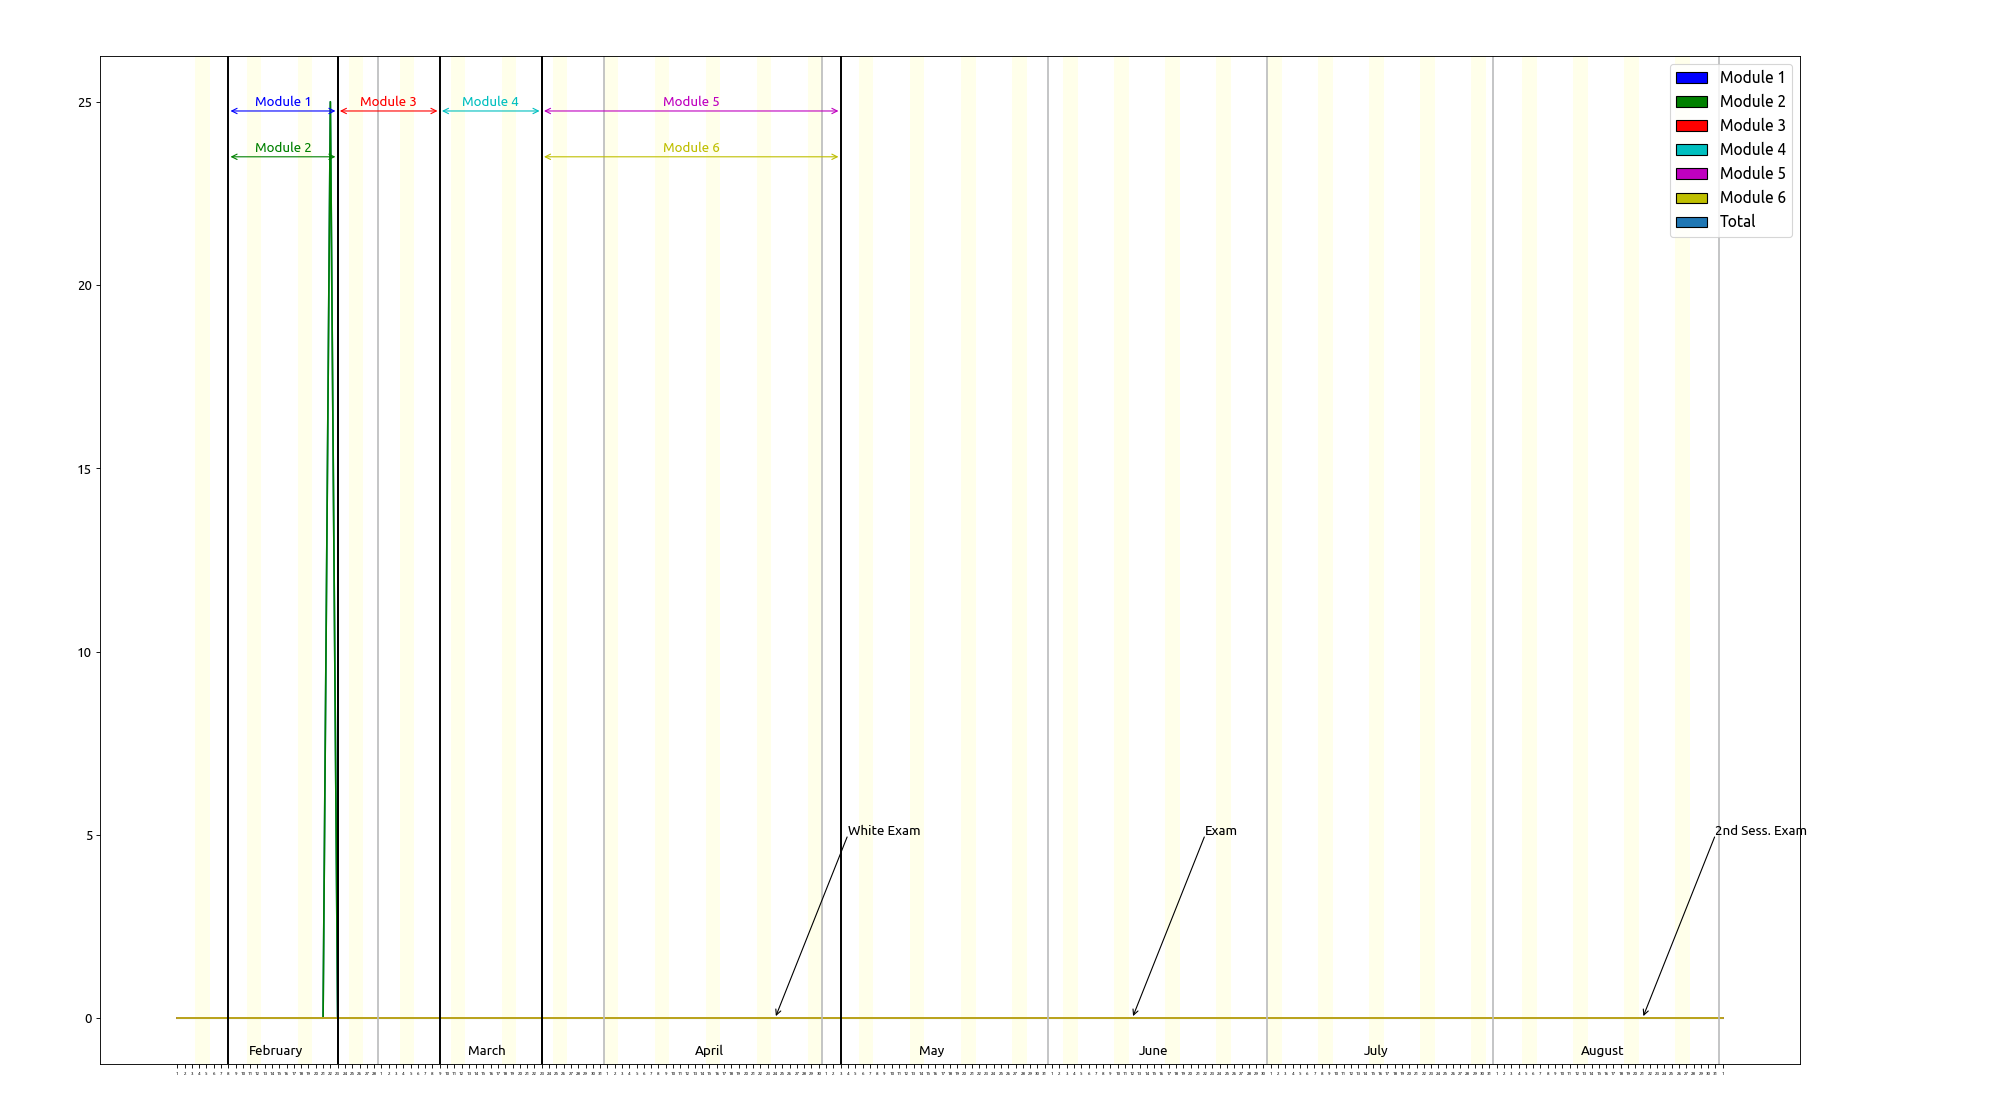
\includegraphics[width=.48\linewidth]{bad_timeline_7110523.png}
  	  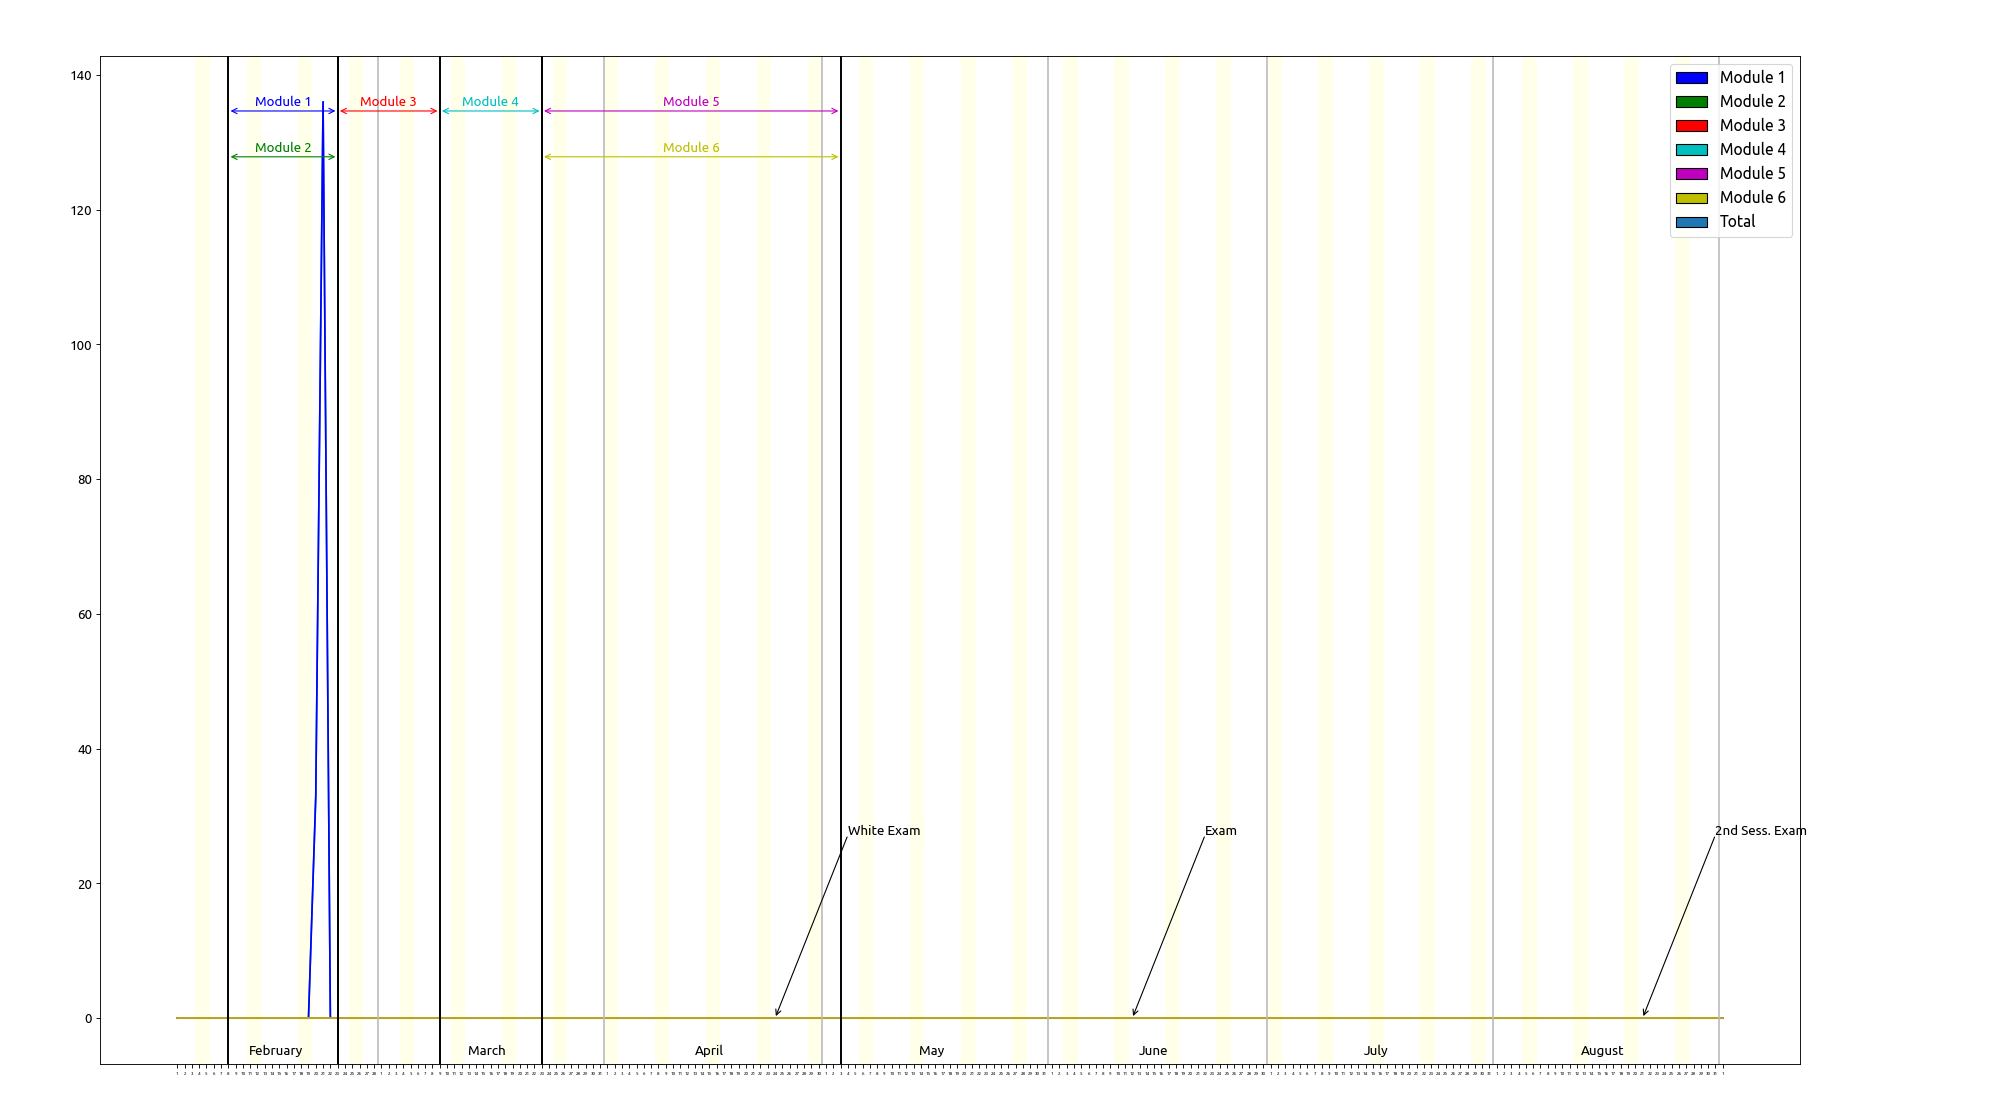
\includegraphics[width=.48\linewidth]{bad_timeline_6370413.png}
      \\
      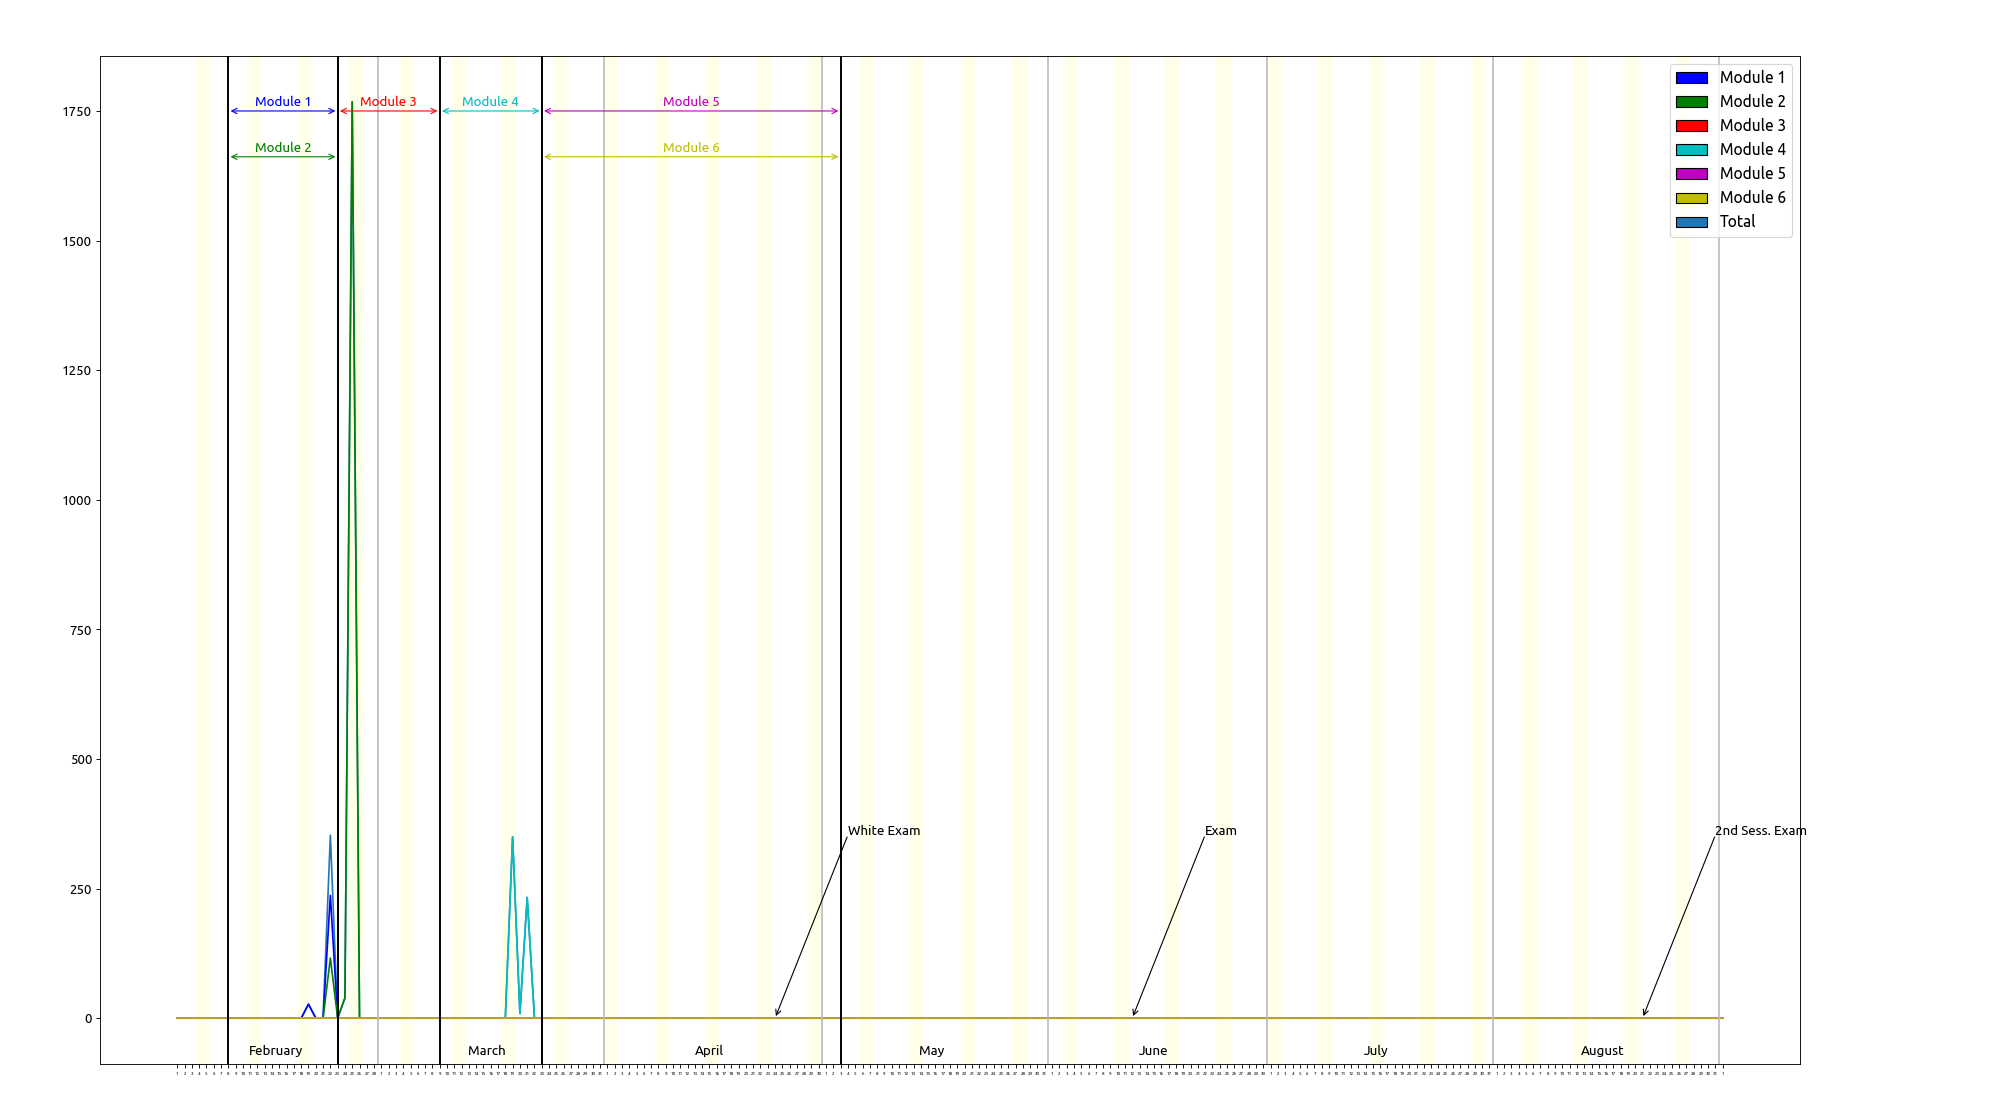
\includegraphics[width=.48\linewidth]{bad_timeline_5897419.png}
      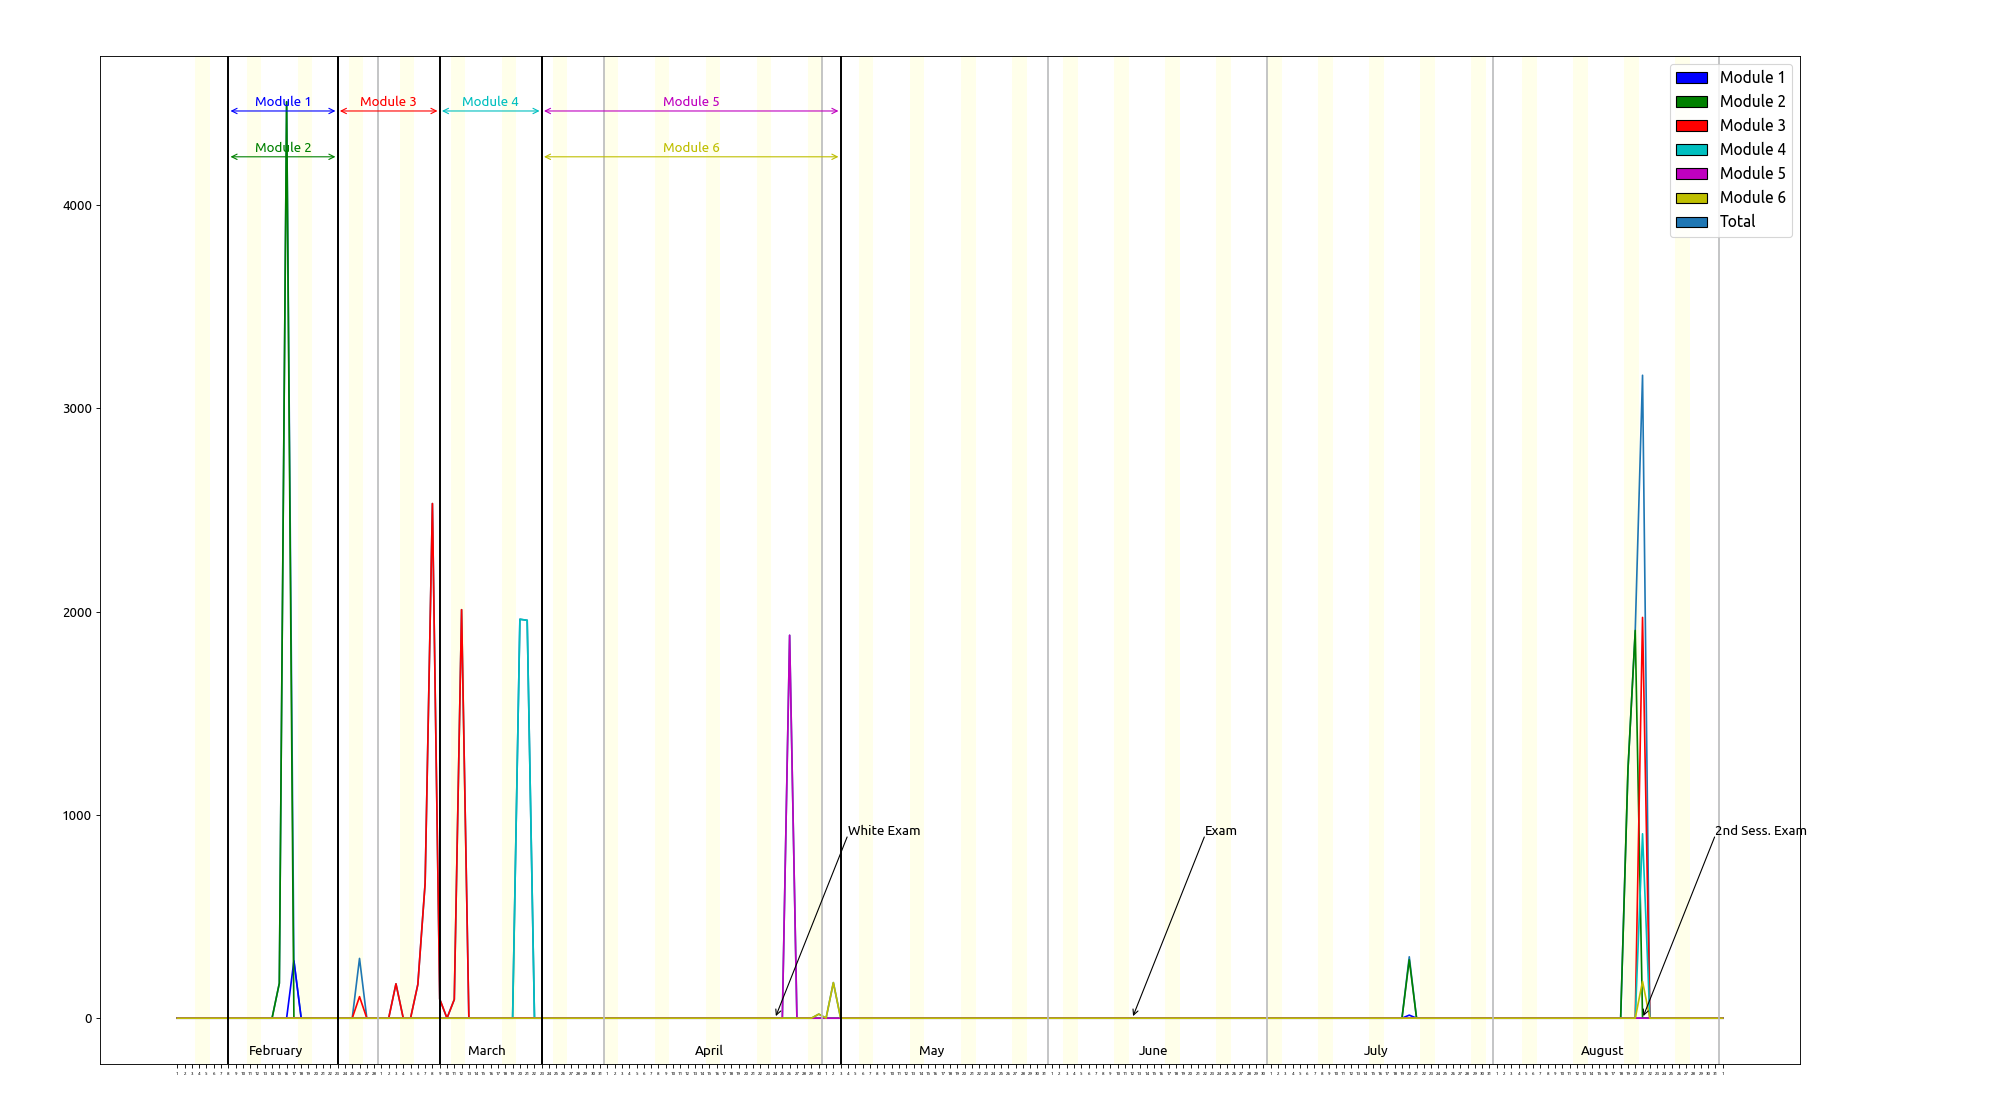
\includegraphics[width=.48\linewidth]{bad_timeline_3905979.png}
      \caption{Timelines of the students with the lowest grades}
      \label{fig:tm1}
      \end{figure}


      \begin{figure}[H]
      \centering
  	  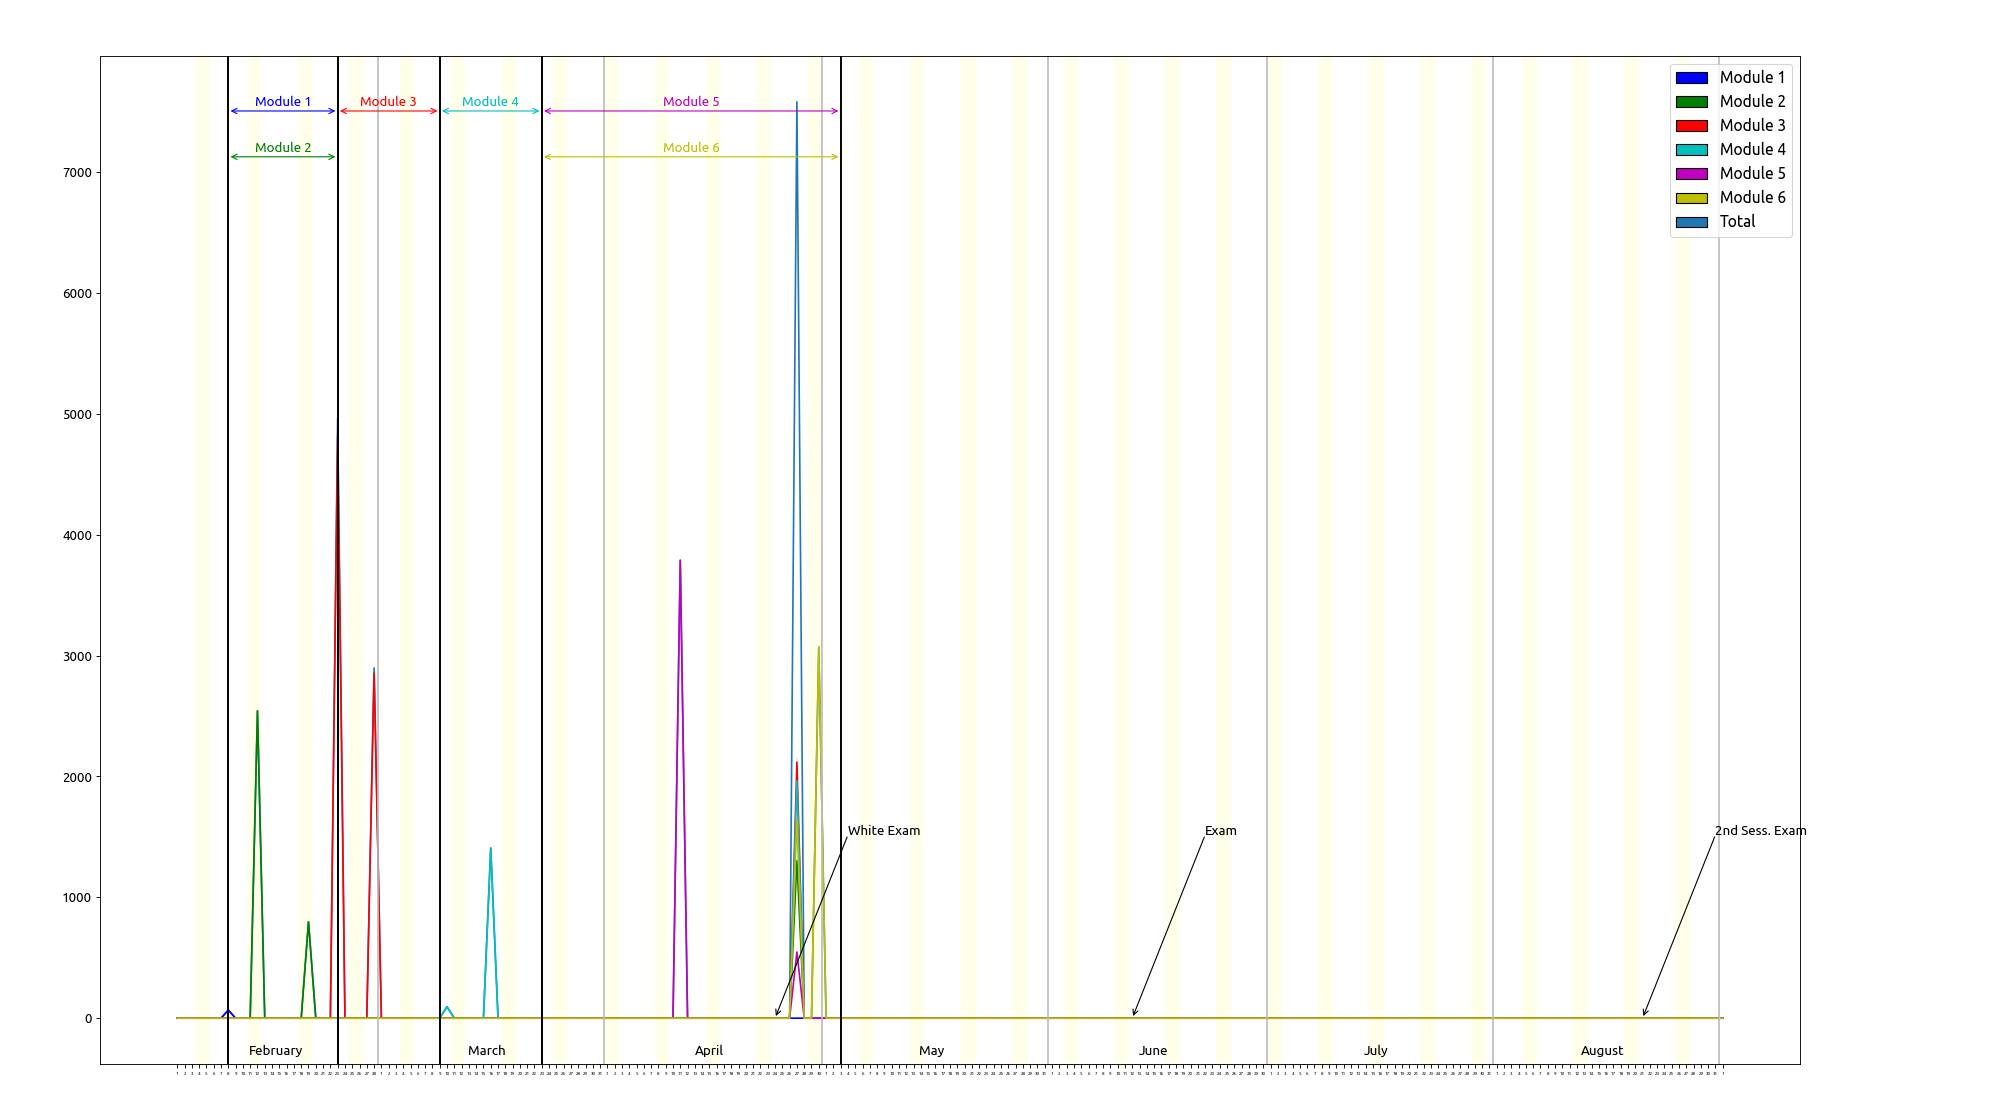
\includegraphics[width=.48\linewidth]{good_timeline_1747564.png}
  	  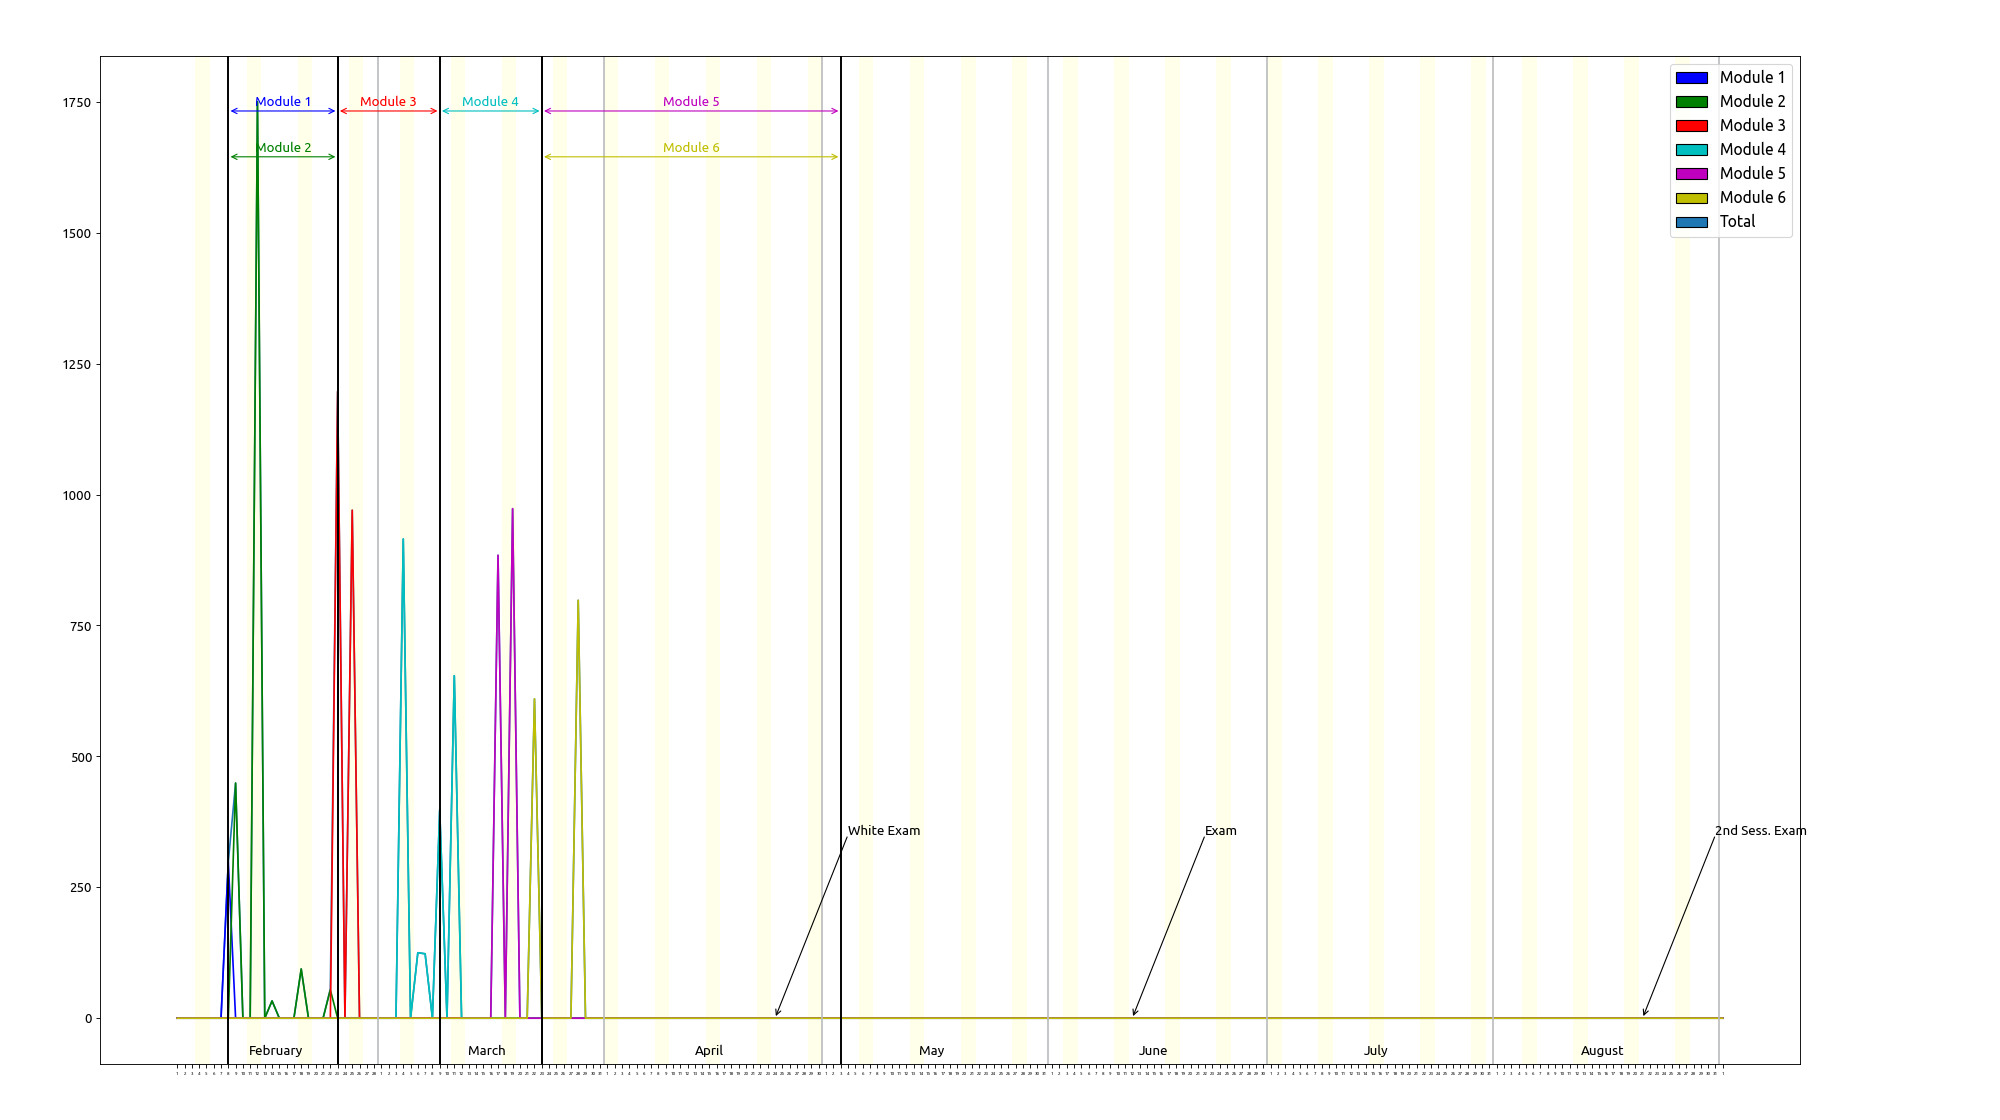
\includegraphics[width=.48\linewidth]{good_timeline_1793969.png}
      \\
      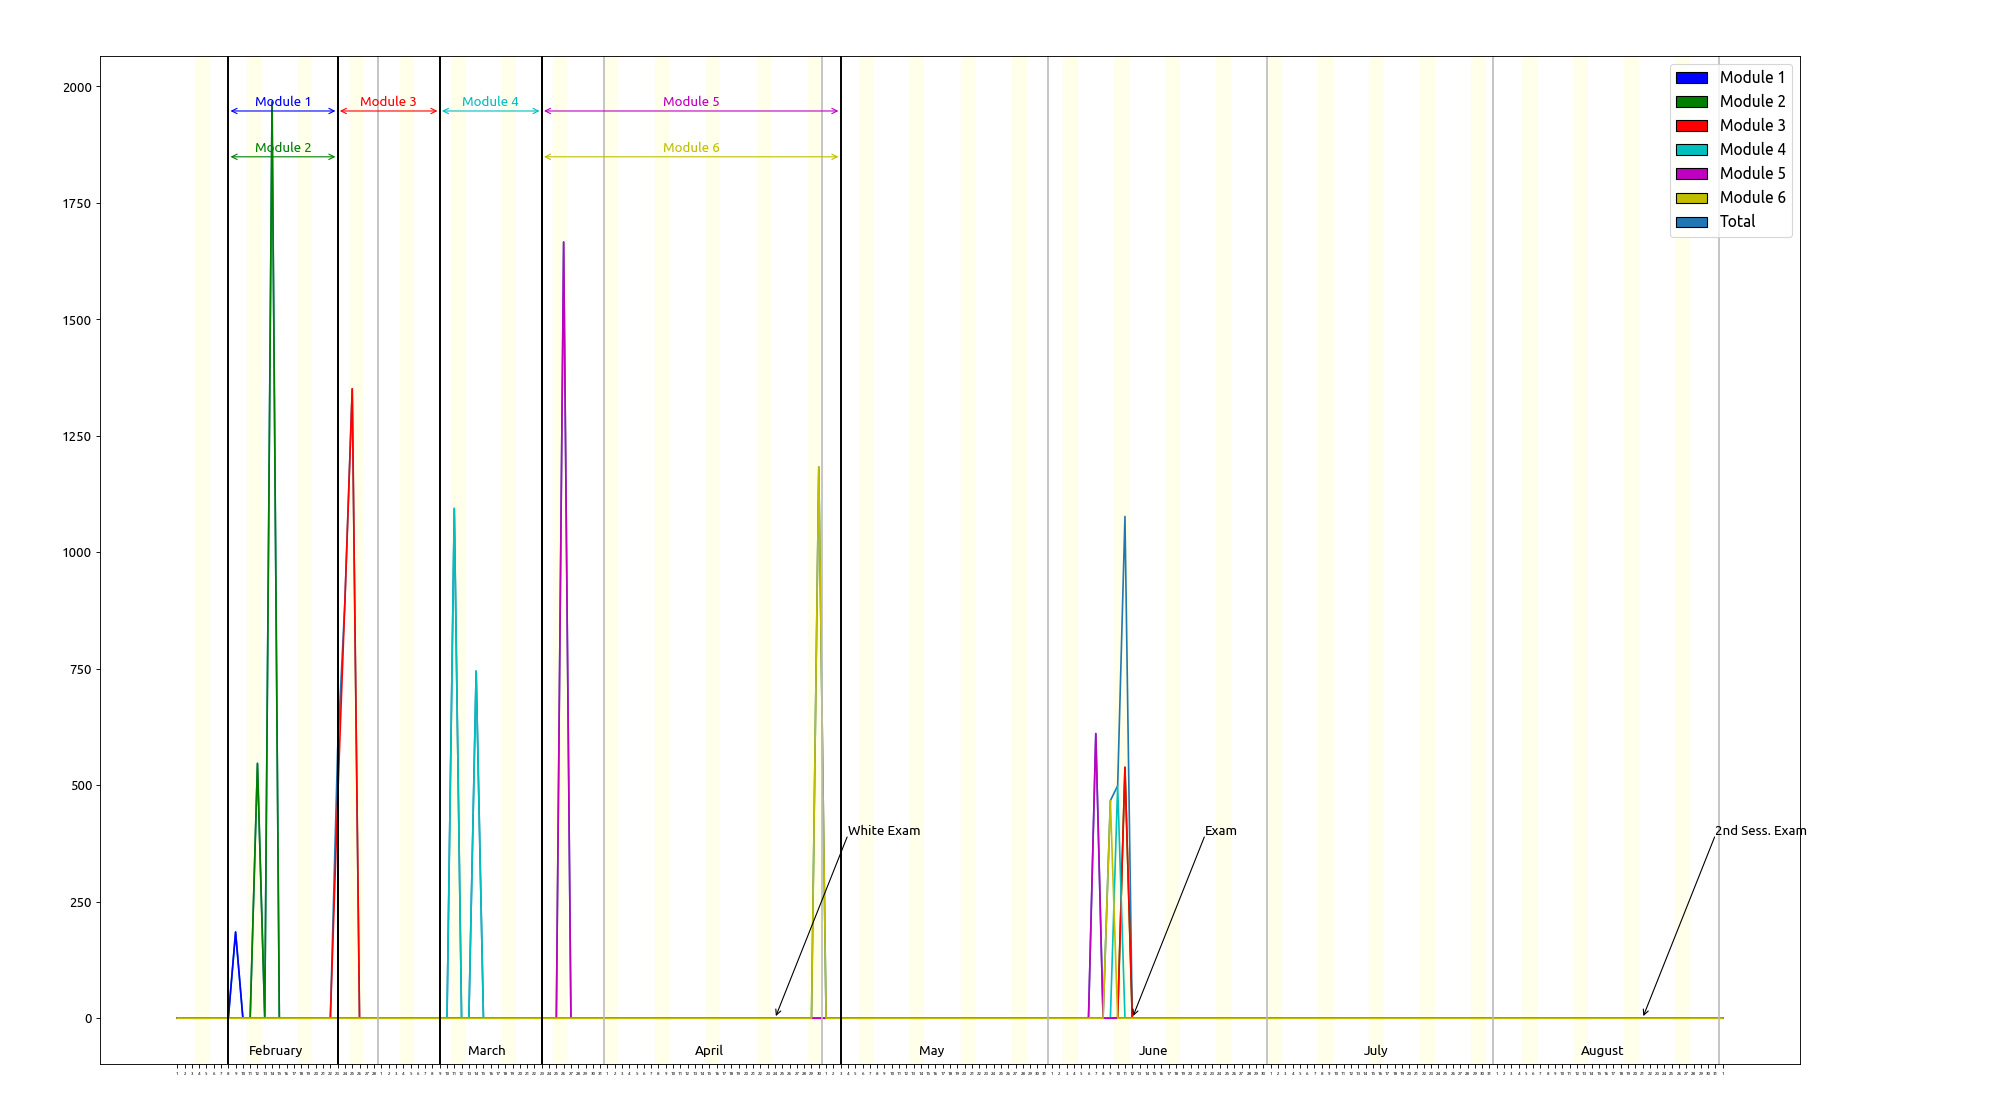
\includegraphics[width=.48\linewidth]{good_timeline_1942114.png}
      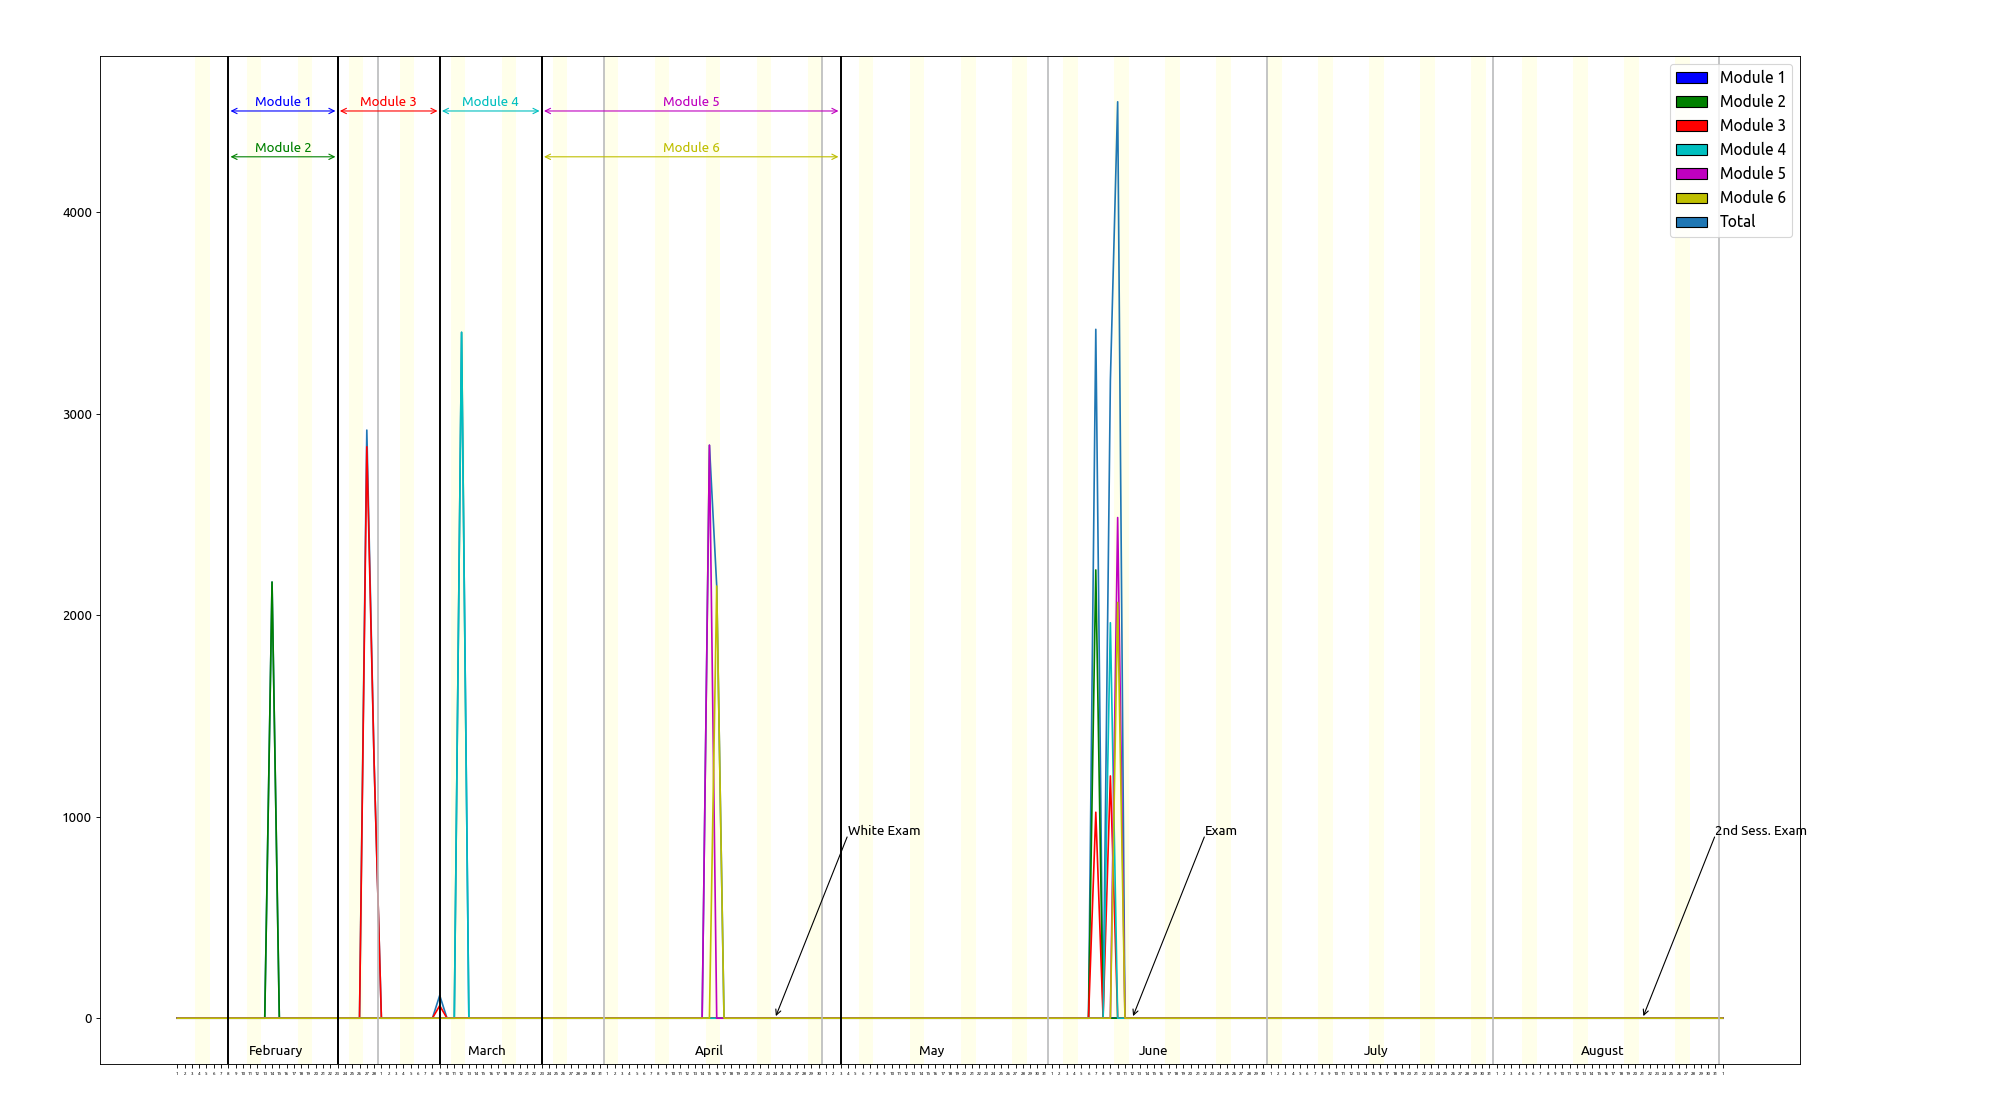
\includegraphics[width=.48\linewidth]{good_timeline_3554348.png}
      \caption{Timelines of the students with the highest grades}
      \label{fig:tm2}
      \end{figure}

    For the timelines of students with the lowest grades, for the mostpart it's pretty straightforward.
    There are are a small number of positions and some modules were not even visited.
    There is one student who followed different patterns with a respectable activity.
    Unfortunately, the student still failed the exam.\\

    Meanwhile, for the students with th highest grades, there are many more positions as a whole.
    Also, images for all the modules were visited.
    There is a clear difference between the two sets.
    But in the set of students with the highest grades, there are many different patterns.
    Some students have a significant higher activity than others.
    One worked on modules ahead of time, and some didn't even log onto Cytomine the weeks before the exam.
    This shows that it's hard to judge a student's performance and comprehension of the course.
    Students follow different habbits and exhibit different patterns.
    There is no "best" method for studying according to this small study.
    The Machine Learning can give more insight on this question.



    \subsubsection{White Test Grades}
    
    These 3 ungraded exam were taken halfway during the semester (24th of April 2017).
    They reflect what a student has learned and remembered up until that day.
    At that point, students should have finished modules 1 through 4 and at least looked at modules 5 and 6.
    These tests could be a great indicator on how well students can perform during the real exam.
    These \textbf{Y} variables were tested using a Leave-one-out cross validation on an Extra Tree Regressor with the generated data set.
    As a reminder, scores are calculated with the Mean Absolute Error technique.
    Also, the results are also compared with a model that learns by simply using the median.
    This is to determine if the model has much merit. (Figure \ref{fig:results_white})
    \begin{figure}[H]
      \centering
  	  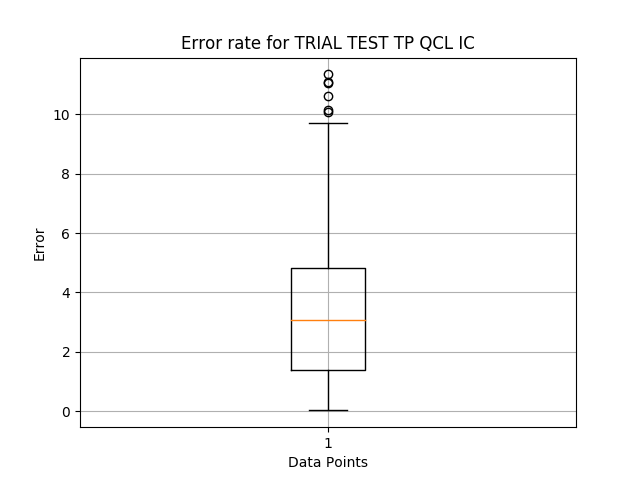
\includegraphics[width=.3\linewidth]{cv_boxplot_TRIAL_TEST_TP_QCL_IC_2018-04-27_14_35_12.png}
  	  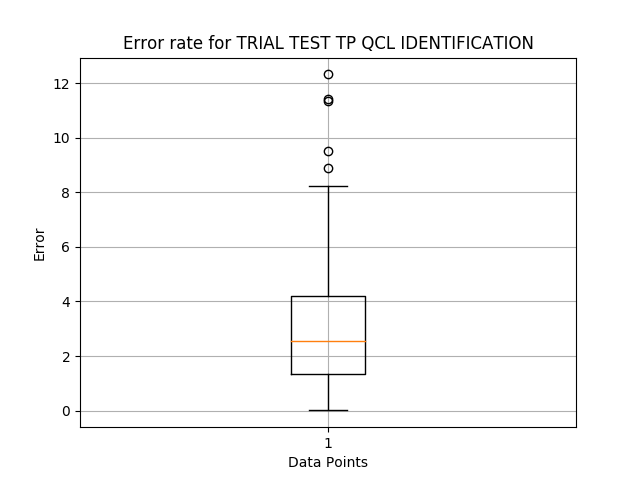
\includegraphics[width=.3\linewidth]{cv_boxplot_TRIAL_TEST_TP_QCL_IDENTIFICATION_2018-04-27_14_31_56.png}
      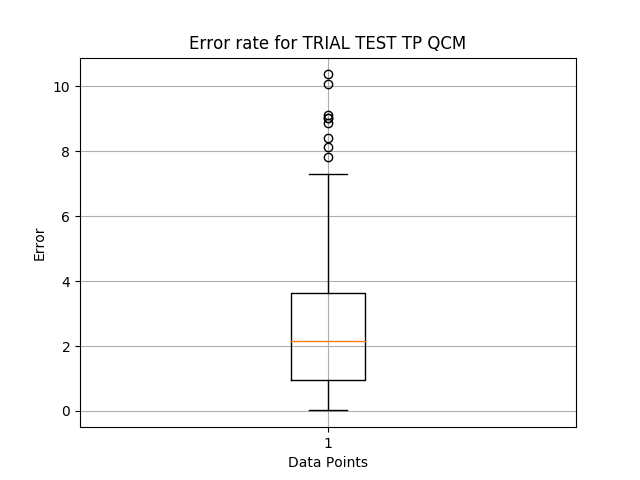
\includegraphics[width=.3\linewidth]{cv_boxplot_TRIAL_TEST_TP_QCM_2018-04-27_17_16_59.png}
      \\
      \ref{fig:results_white}.1: Boxplots of the error values
      \\
      \vspace{0.5cm}
      \begin{tabular}{| l | c | c | c | c | c |}
      \hline
      & \tiny{Score} & \tiny{Median Score} & \tiny{Score Difference} & \tiny{Real Median Grade} & \tiny{Median Est.
      Grade}\\ \hline
      \tiny{QCL incidence white test} & \tiny{3.44} & \tiny{3.37} & \tiny{-0.08} & \tiny{13.33} & \tiny{12.321765}\\ \hline
      \tiny{QCL identification white test} & \tiny{2.99} & \tiny{3.10} & \tiny{0.11} & \tiny{8.0} & \tiny{8.36}\\ \hline
      \tiny{Practical QCM white test} & \tiny{2.58} & \tiny{2.57} & \tiny{-0.004} & \tiny{10.36} & \tiny{10.29}\\
      \hline
      \end{tabular}\\
      \vspace{0.5cm}
      \ref{fig:results_white}.2: Discrete Results\\
      \vspace{0.3cm}
      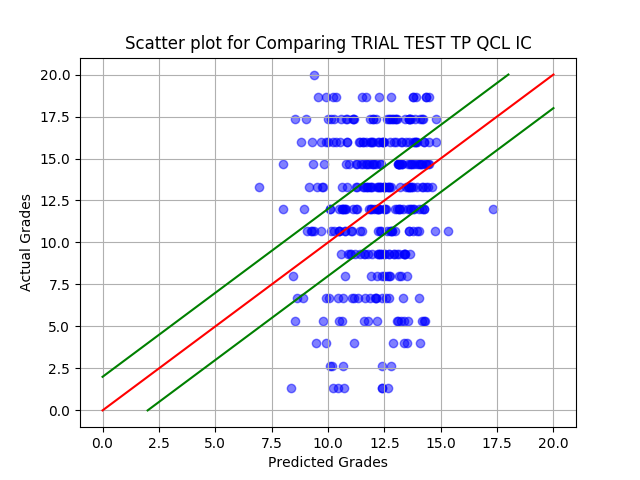
\includegraphics[width=.3\linewidth]{cv_comp_TRIAL_TEST_TP_QCL_IC_2018-04-27_14_35_12.png}
  	  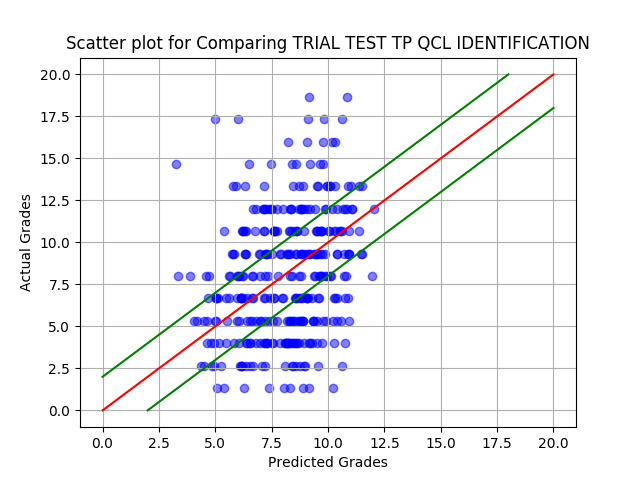
\includegraphics[width=.3\linewidth]{cv_comp_TRIAL_TEST_TP_QCL_IDENTIFICATION_2018-04-27_14_31_55.png}
      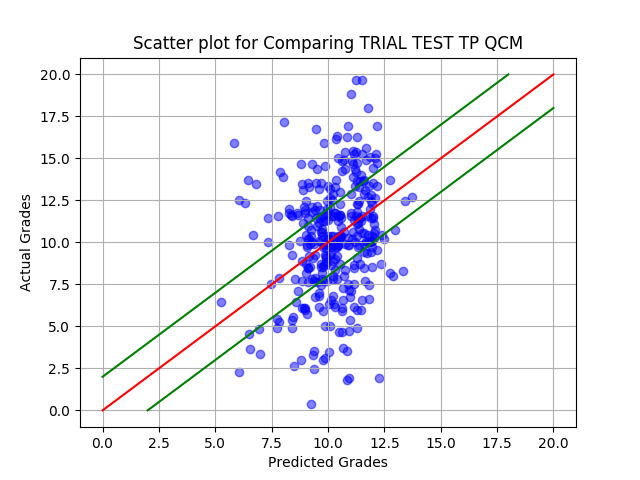
\includegraphics[width=.3\linewidth]{cv_comp_TRIAL_TEST_TP_QCM_2018-04-27_17_16_59.png}
      \\
      \ref{fig:results_white}.3: Actual grades compared to Predicated grades
      \caption{Results from cross-validation of the White Tests}
      \label{fig:results_white}
    \end{figure}
    
    Unfortunately, the results are not great.
    The boxplots show very high median and quartiles.
    There are also a high number of extreme errors with some above 10.
    The scores represent the average error of the cross validation.
    With scores nearing nearing 3, in some cases, it's better to try and guess using the median value.
    For the incidence test, it seems that the scores are underestimated, this seems to be the case because there is a significantly high grades compared to low grades.
    There are many reasons why results are the way they are.
    This includes the fact that these grades do not rely on activity that occur after the exam date.
    When comparing grade the learned grades against the original grades, it's noticeable that the estimated grades tend to predict values close to the average of the actual grades.
    This makes it so that high and low actual grades when predicted tend to be more erroneous.
    The sample also lacks a good amount of extreme grades which gives the algorithm less to work with for these cases.
    Furthermore, the fact that the exams are ungraded puts less pressure on the students to succeed.
    Therefore, they might not take the tests as seriously as they could by not reviewing and studying the days before. \\
    %%todo add reference to timeline    
  
  Since the models are made using regression trees, it it possible to study the features that had an impact in determining the predicted grades.
  Even though the results were not ideal, it's interesting to observe what images and variables had a big impact on determining the grades.
  These images can very well be the subject of a question on the exam. (Figures \ref{fig:var_white1}, \ref{fig:var_white2}, \ref{fig:var_white3})

     \begin{figure}[H]
      \centering
      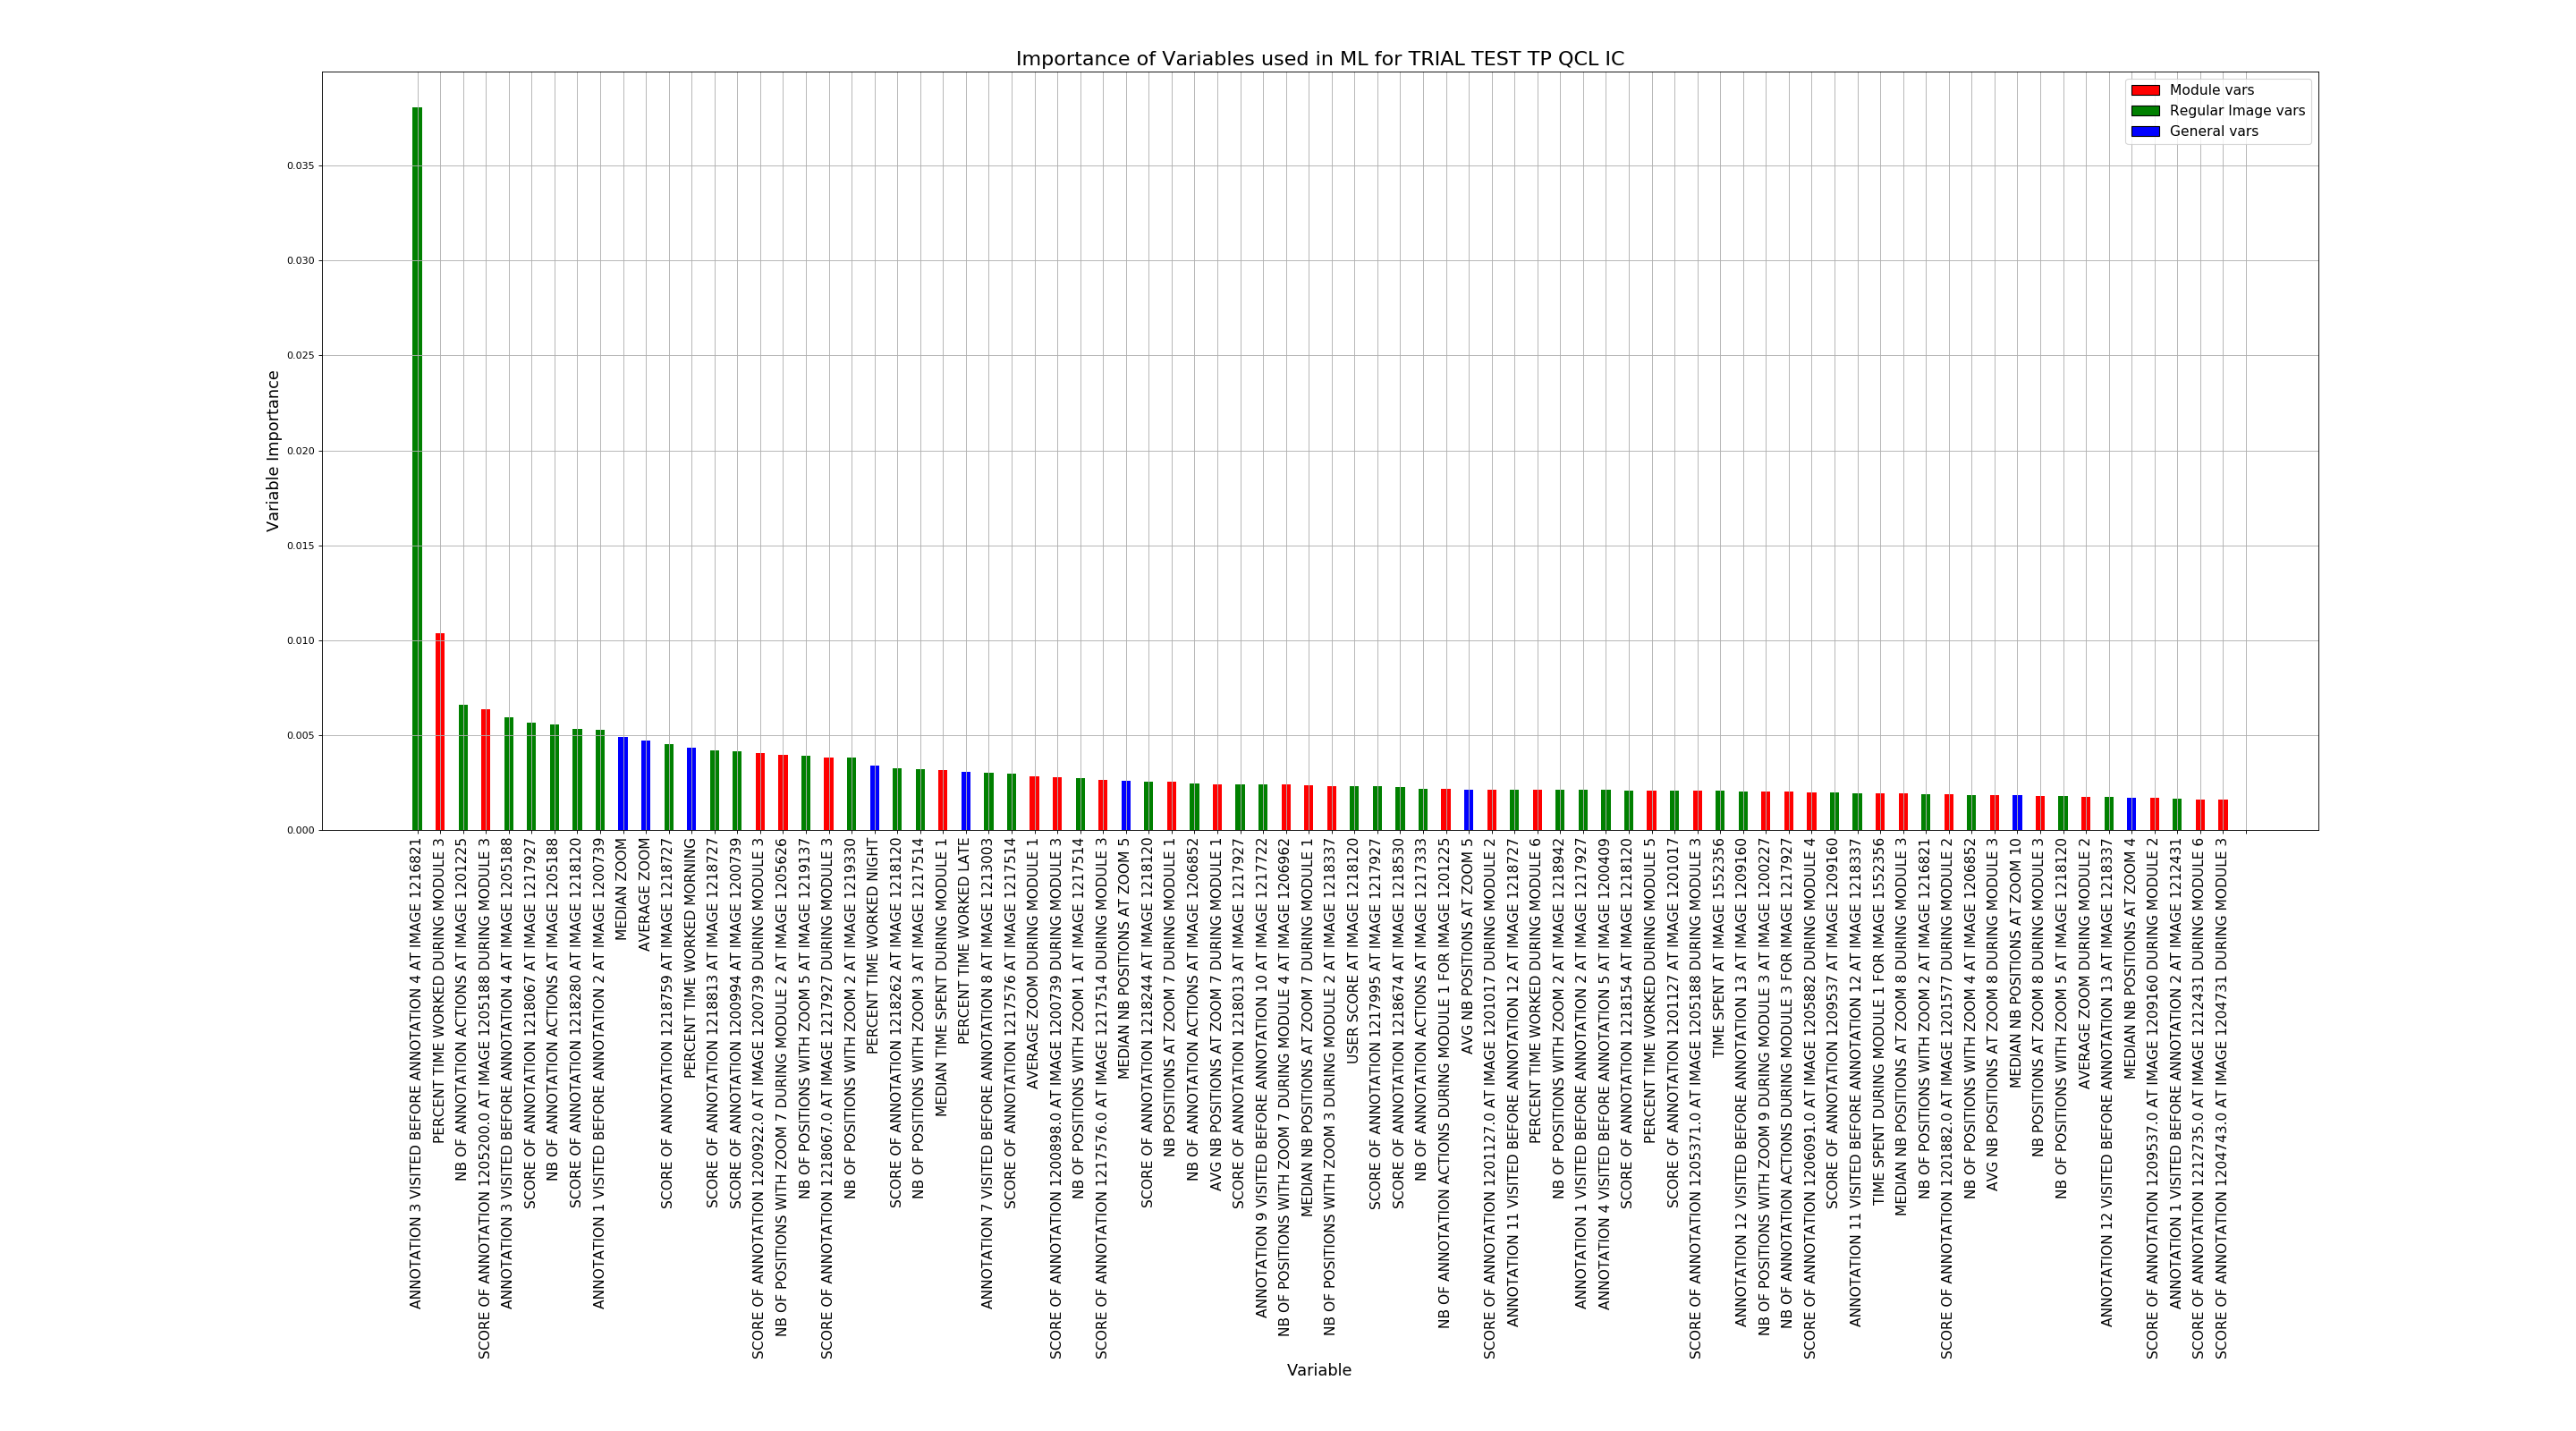
\includegraphics[width=.95\linewidth]{var_importance_TRIAL_TEST_TP_QCL_IC_2018-04-29_14_31_17.png}
      \caption{Feature Importance for QCL the Incidence}
      \label{fig:var_white1}
      \end{figure}
      
      \begin{figure}[H]
      \centering
      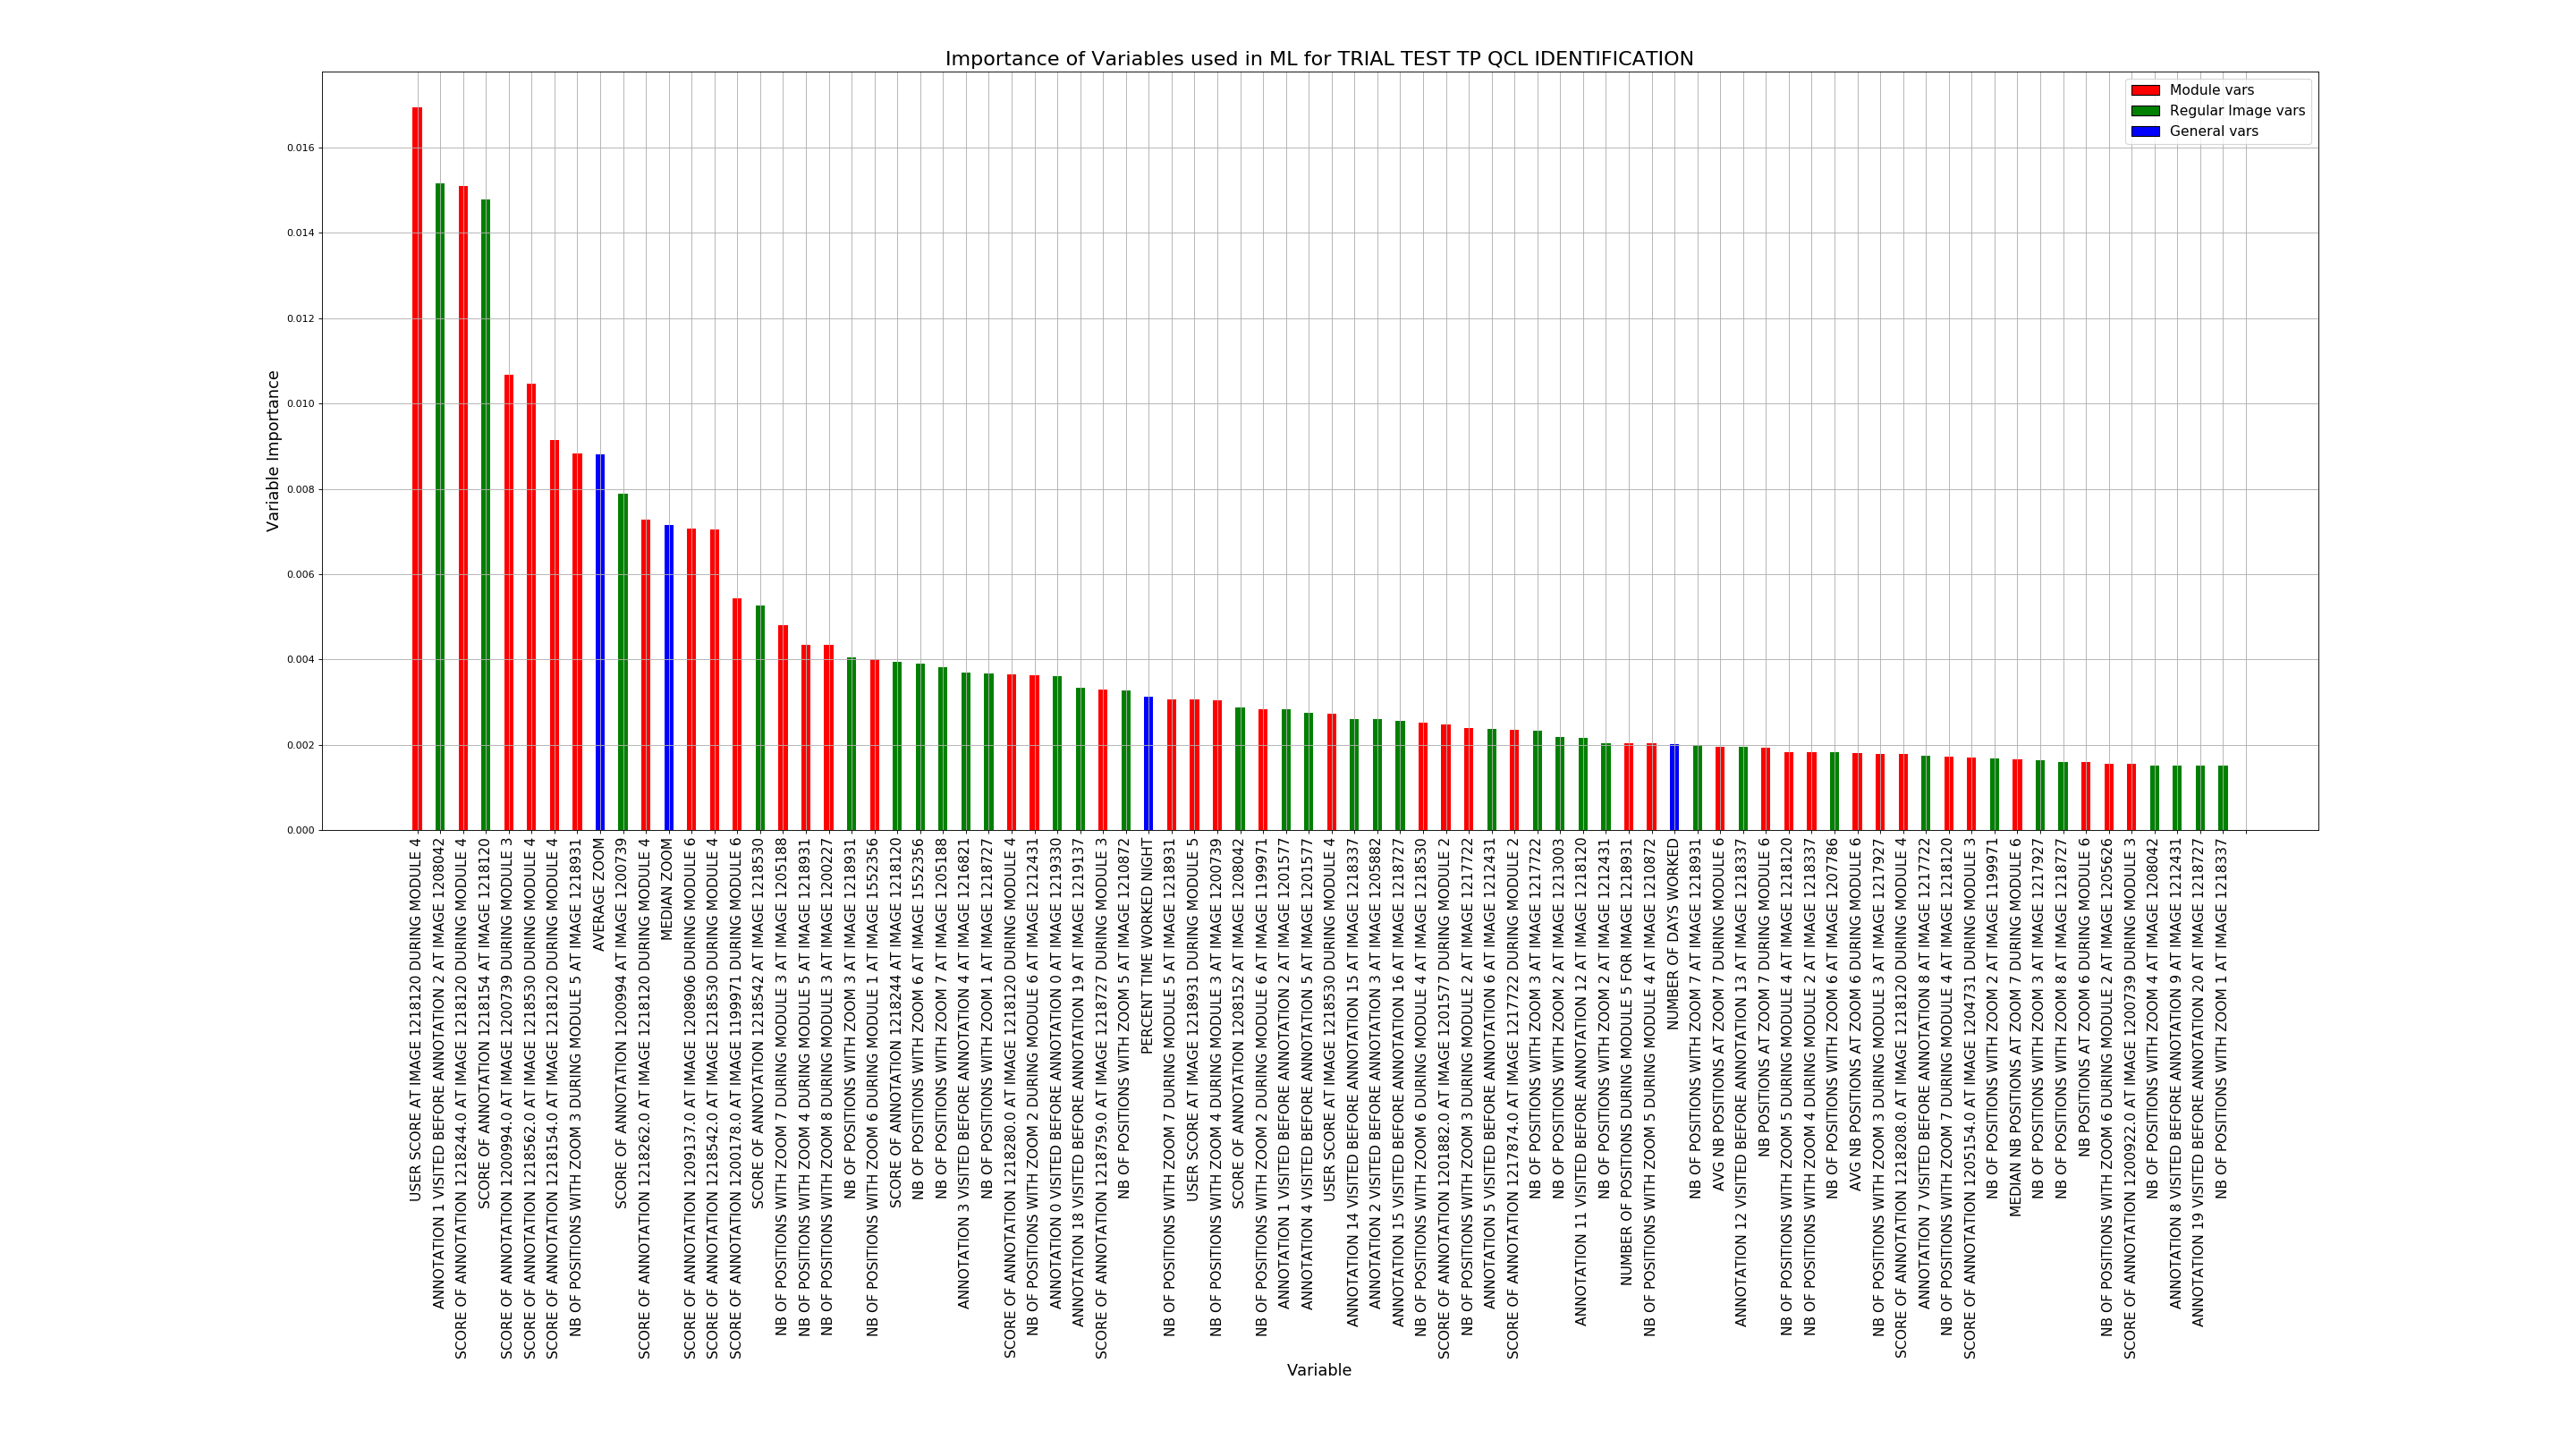
\includegraphics[width=.95\linewidth]{var_importance_TRIAL_TEST_TP_QCL_IDENTIFICATION_2018-04-29_14_28_02.png}
      \caption{Feature Importance for QCL the Identification}
      \label{fig:var_white2}
      \end{figure}
      
      \begin{figure}[H]
      \centering
      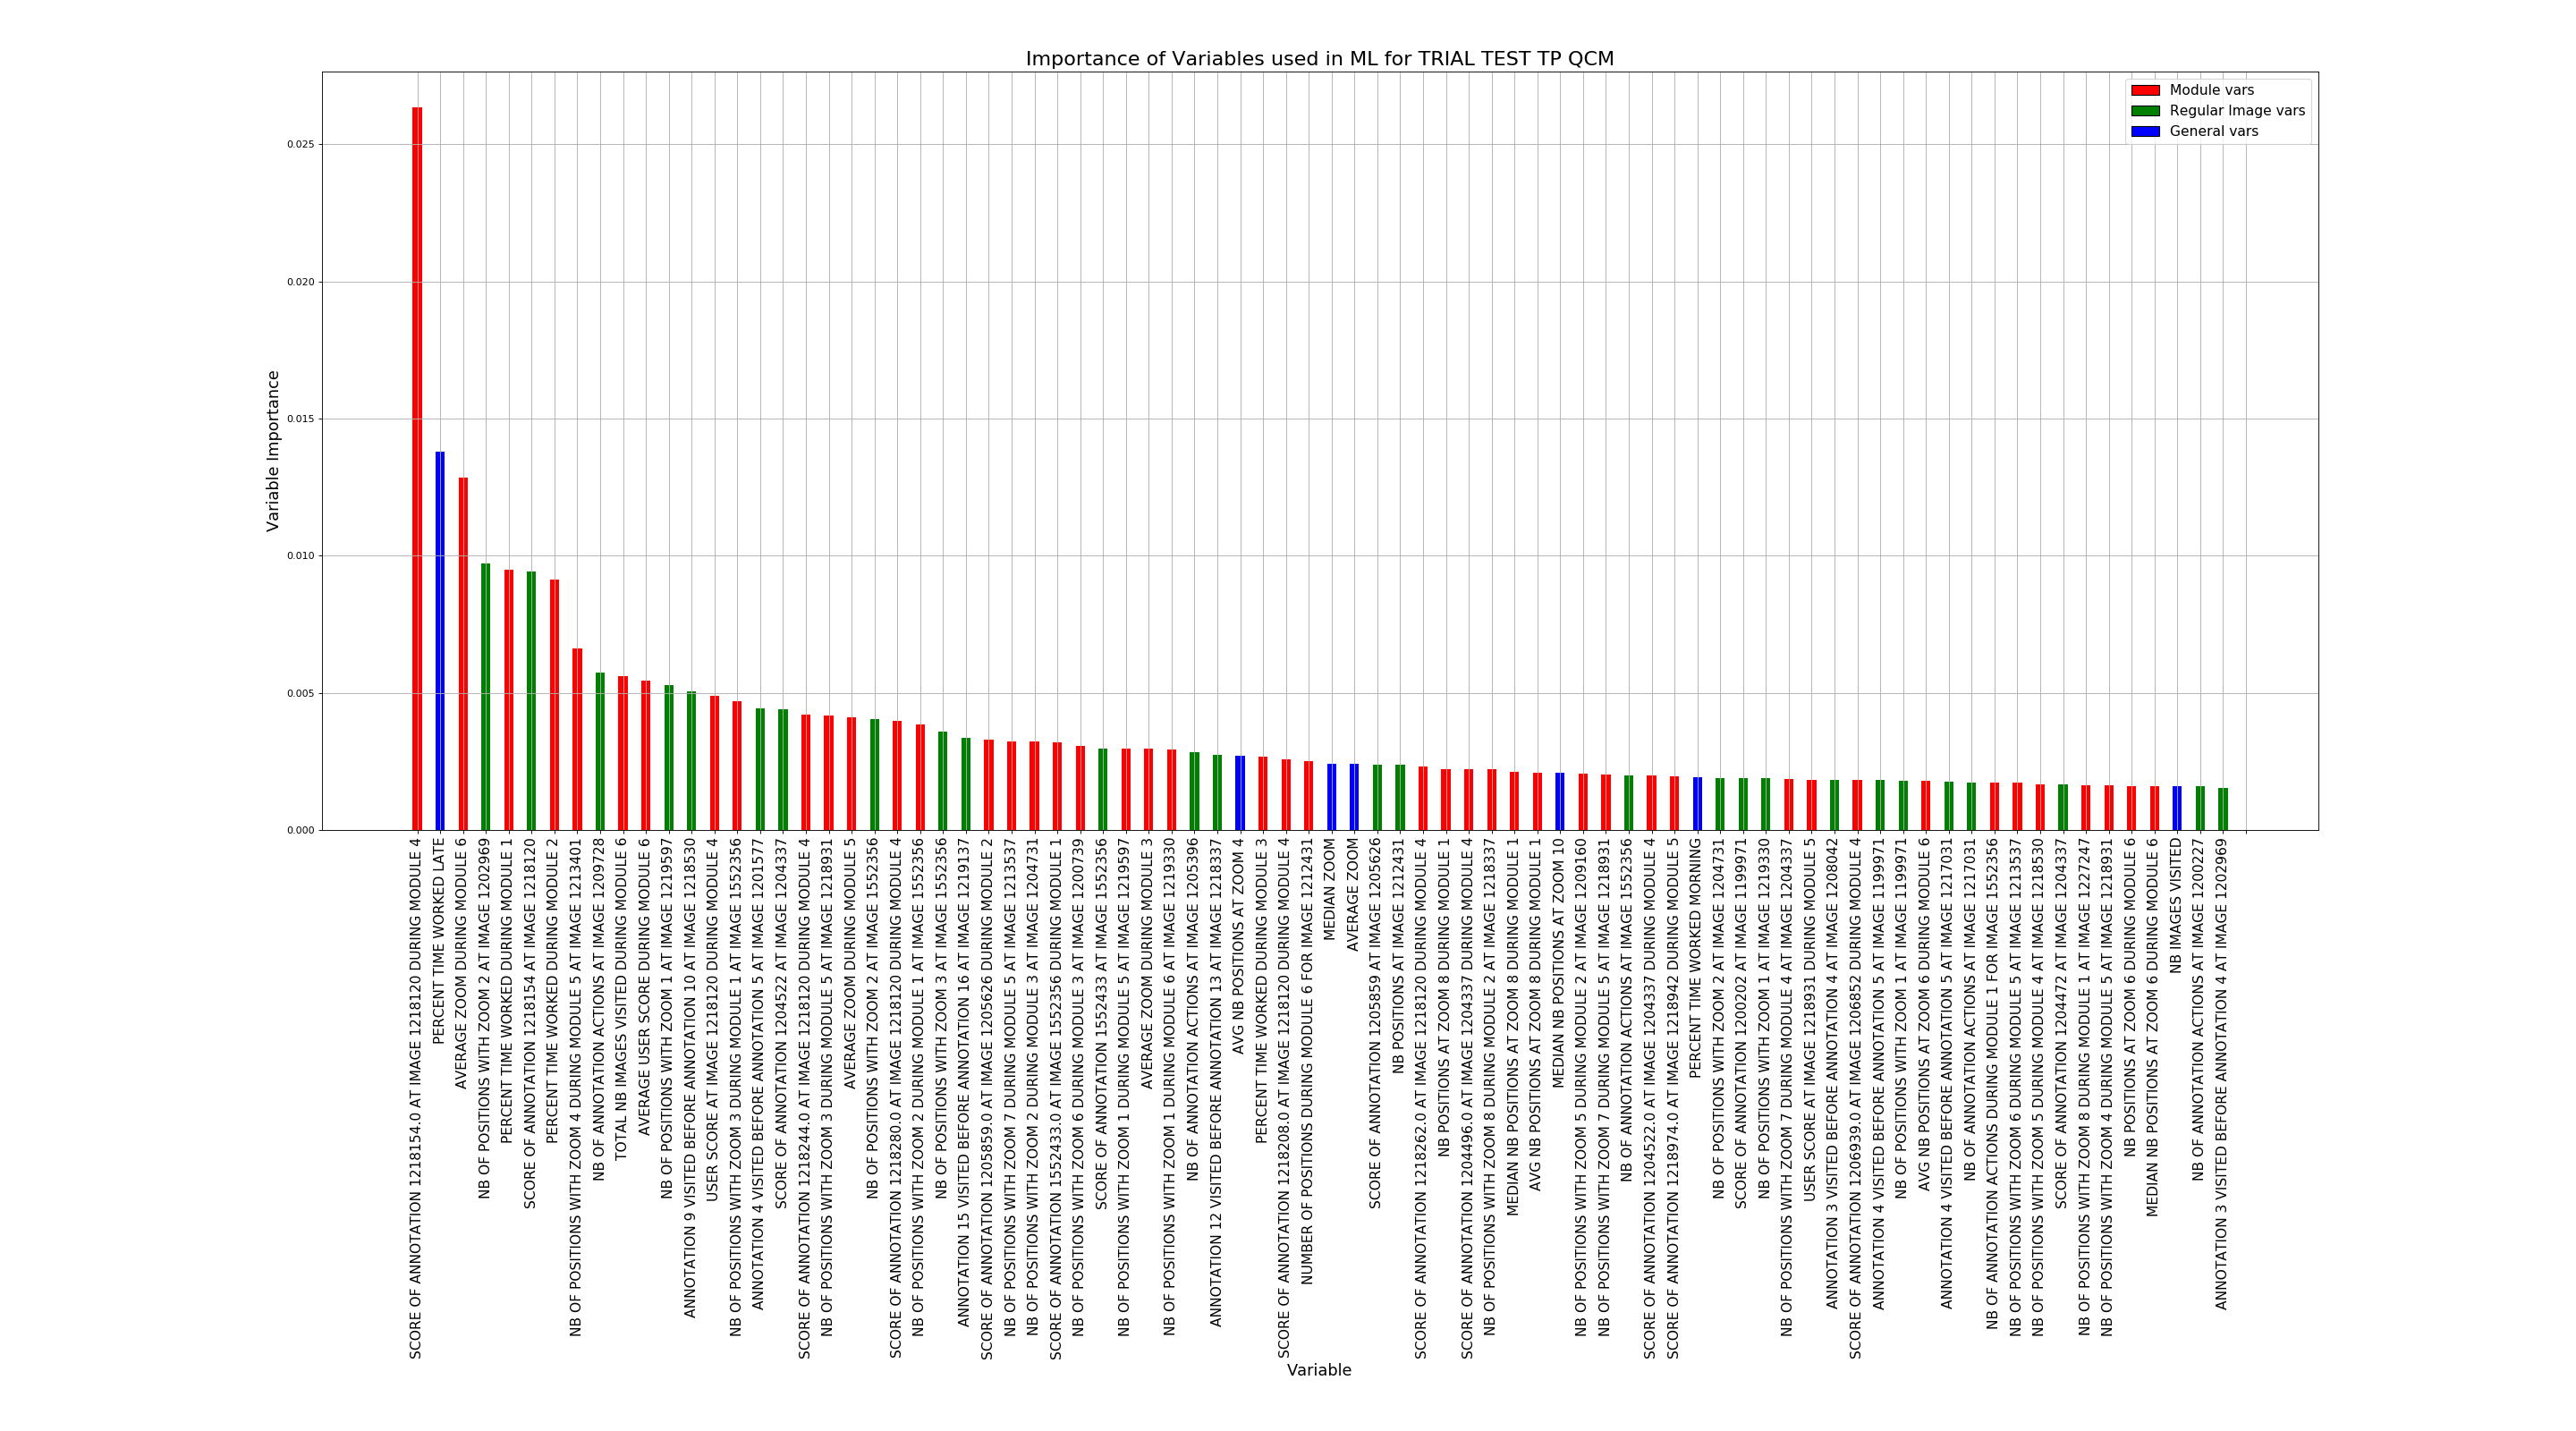
\includegraphics[width=.95\linewidth]{var_importance_TRIAL_TEST_TP_QCM_2018-04-29_14_34_16.png}
      \caption{Feature Importance for the QCM}
      \label{fig:var_white3}
      \end{figure}
    
    These figures show the top 80 features (or \textbf{X} variable) for their respective model.
    Even though each model shares the same features, their importance varies model to model.
    But it's probable that some features from a specific image can be at the top for multiple model.
    Anyways, features are split into 3 categories:
    \begin{itemize}
    \item[\textbullet] General Features : Features that describes the data on the set of images as a whole. (average, median, etc..)
    \item[\textbullet] Regular Image Features : Features that describe the data on a specific image. (number of positions at image XXXX)
    \item[\textbullet] Module Image Features : Features similar to the two previous but associated to a specific module period. (number of positions at image XXXX during module Y)
    \end{itemize}
    
    Note that there are fewer general features, but many of those tend to have a high importance.
    Apart from the incidence test, it's appropriate to say that the module variables are the most impactful.
    This is because the white exam is taken in April instead of June.
    Therefore, user performance during specific modules are better indications on the performance during the white test.
    Also, for the  identification test, the most impactful variable has a much higher importance than the rest.
    Even though this may look random, this variable may well be a good splitting factor.
    Unfortunately, this does not show the overall impact of certain images. (Figures \ref{fig:im_white1}, \ref{fig:im_white2}, \ref{fig:im_white3})
    
      \begin{figure}[H]
      \centering
      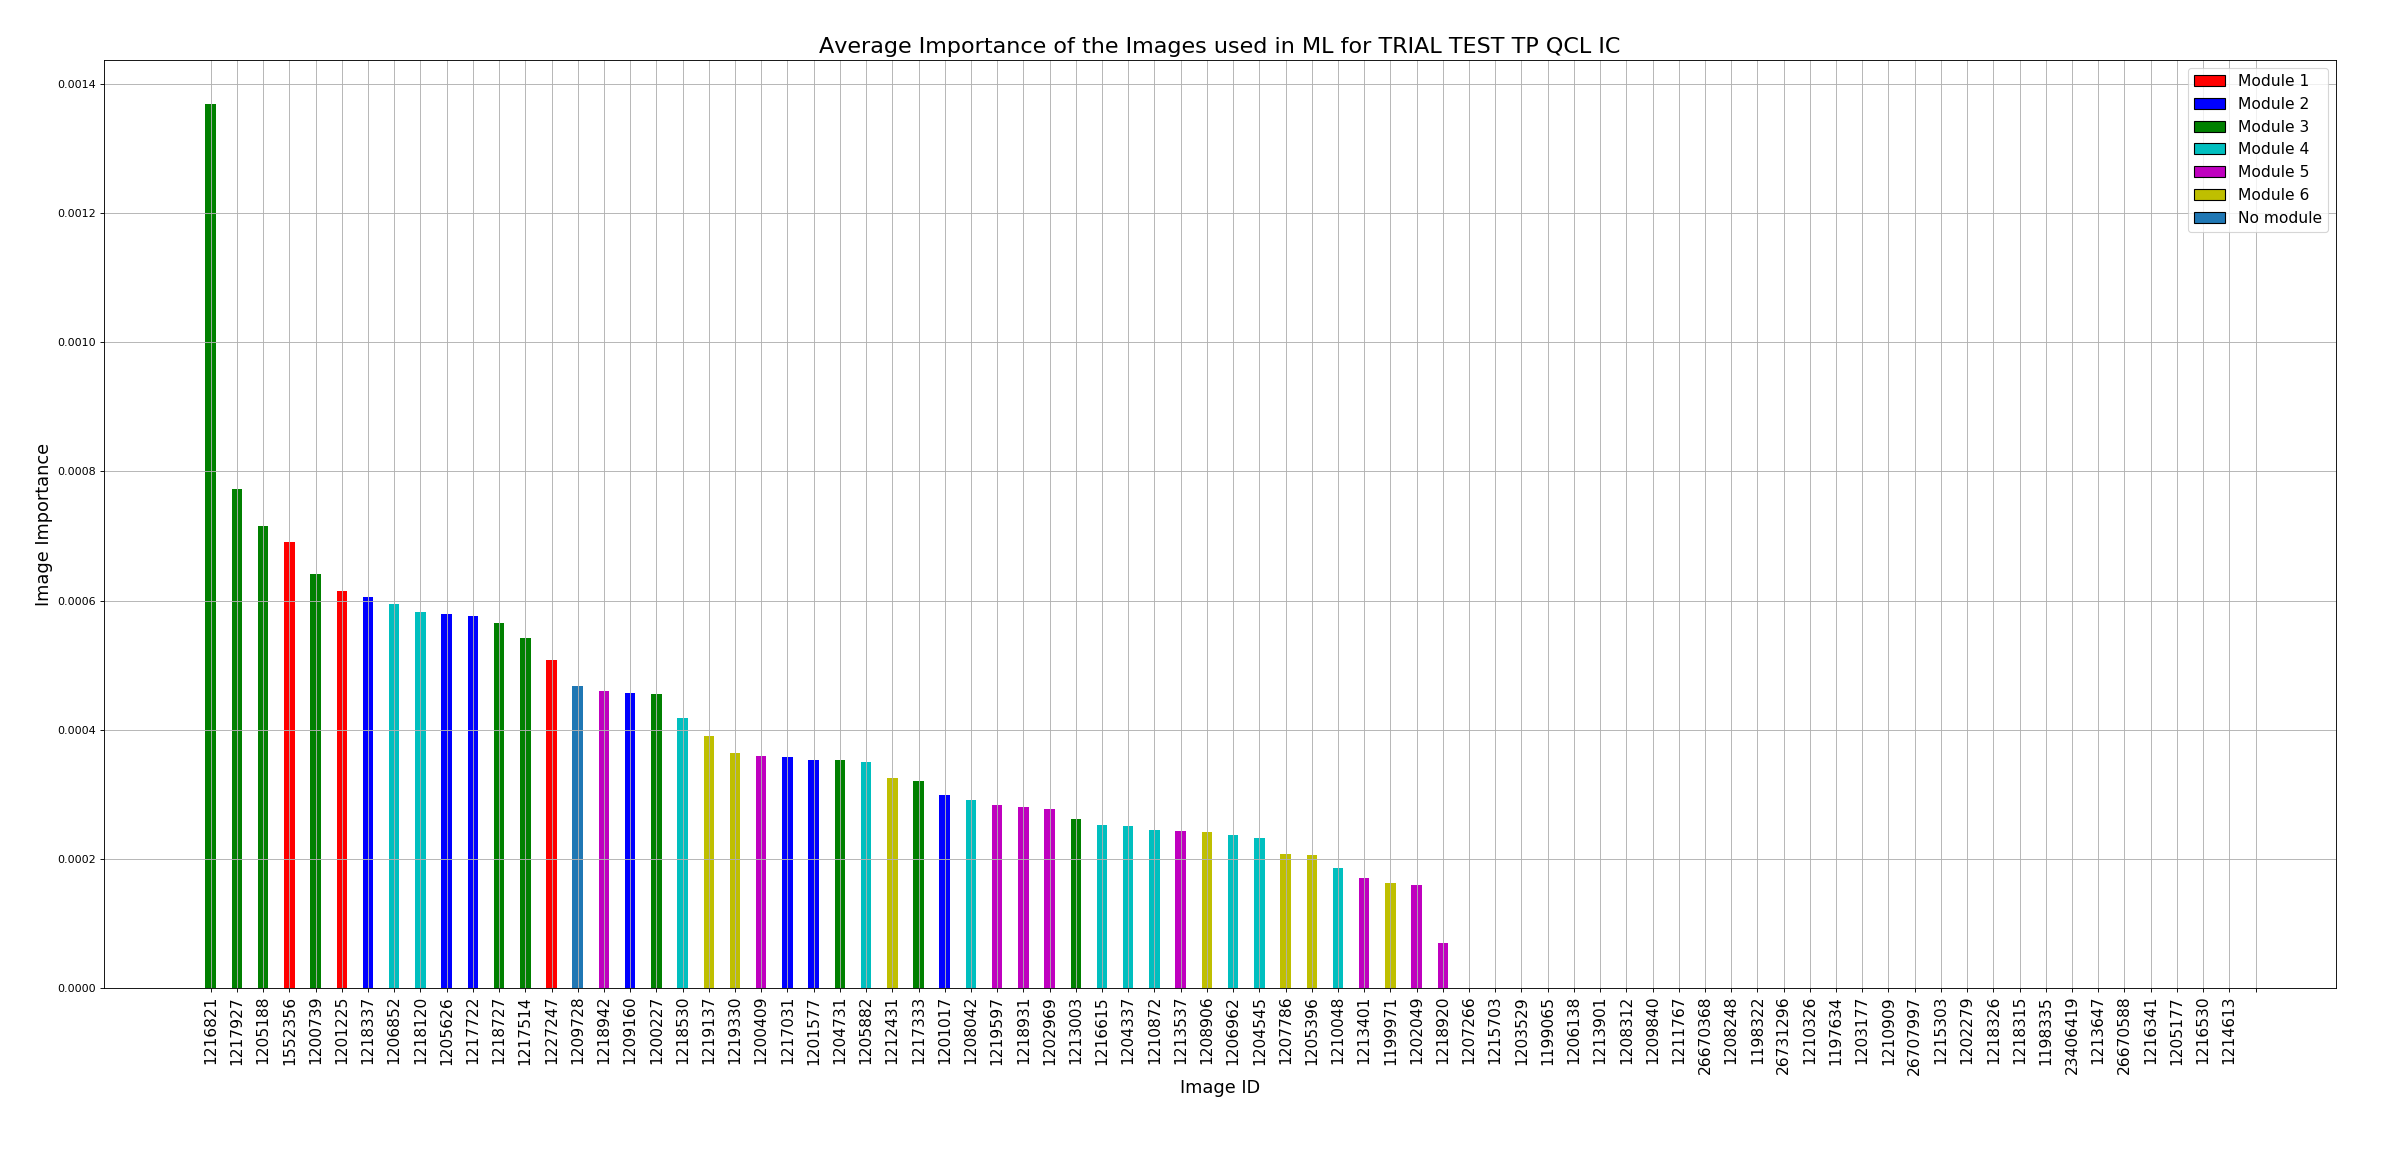
\includegraphics[width=.95\linewidth]{im_importance_TRIAL_TEST_TP_QCL_IC_2018-04-29_14_31_20.png}
      \caption{Image Importance for QCL the Incidence}
      \label{fig:im_white1}
      \end{figure}
      
      \begin{figure}[H]
      \centering
      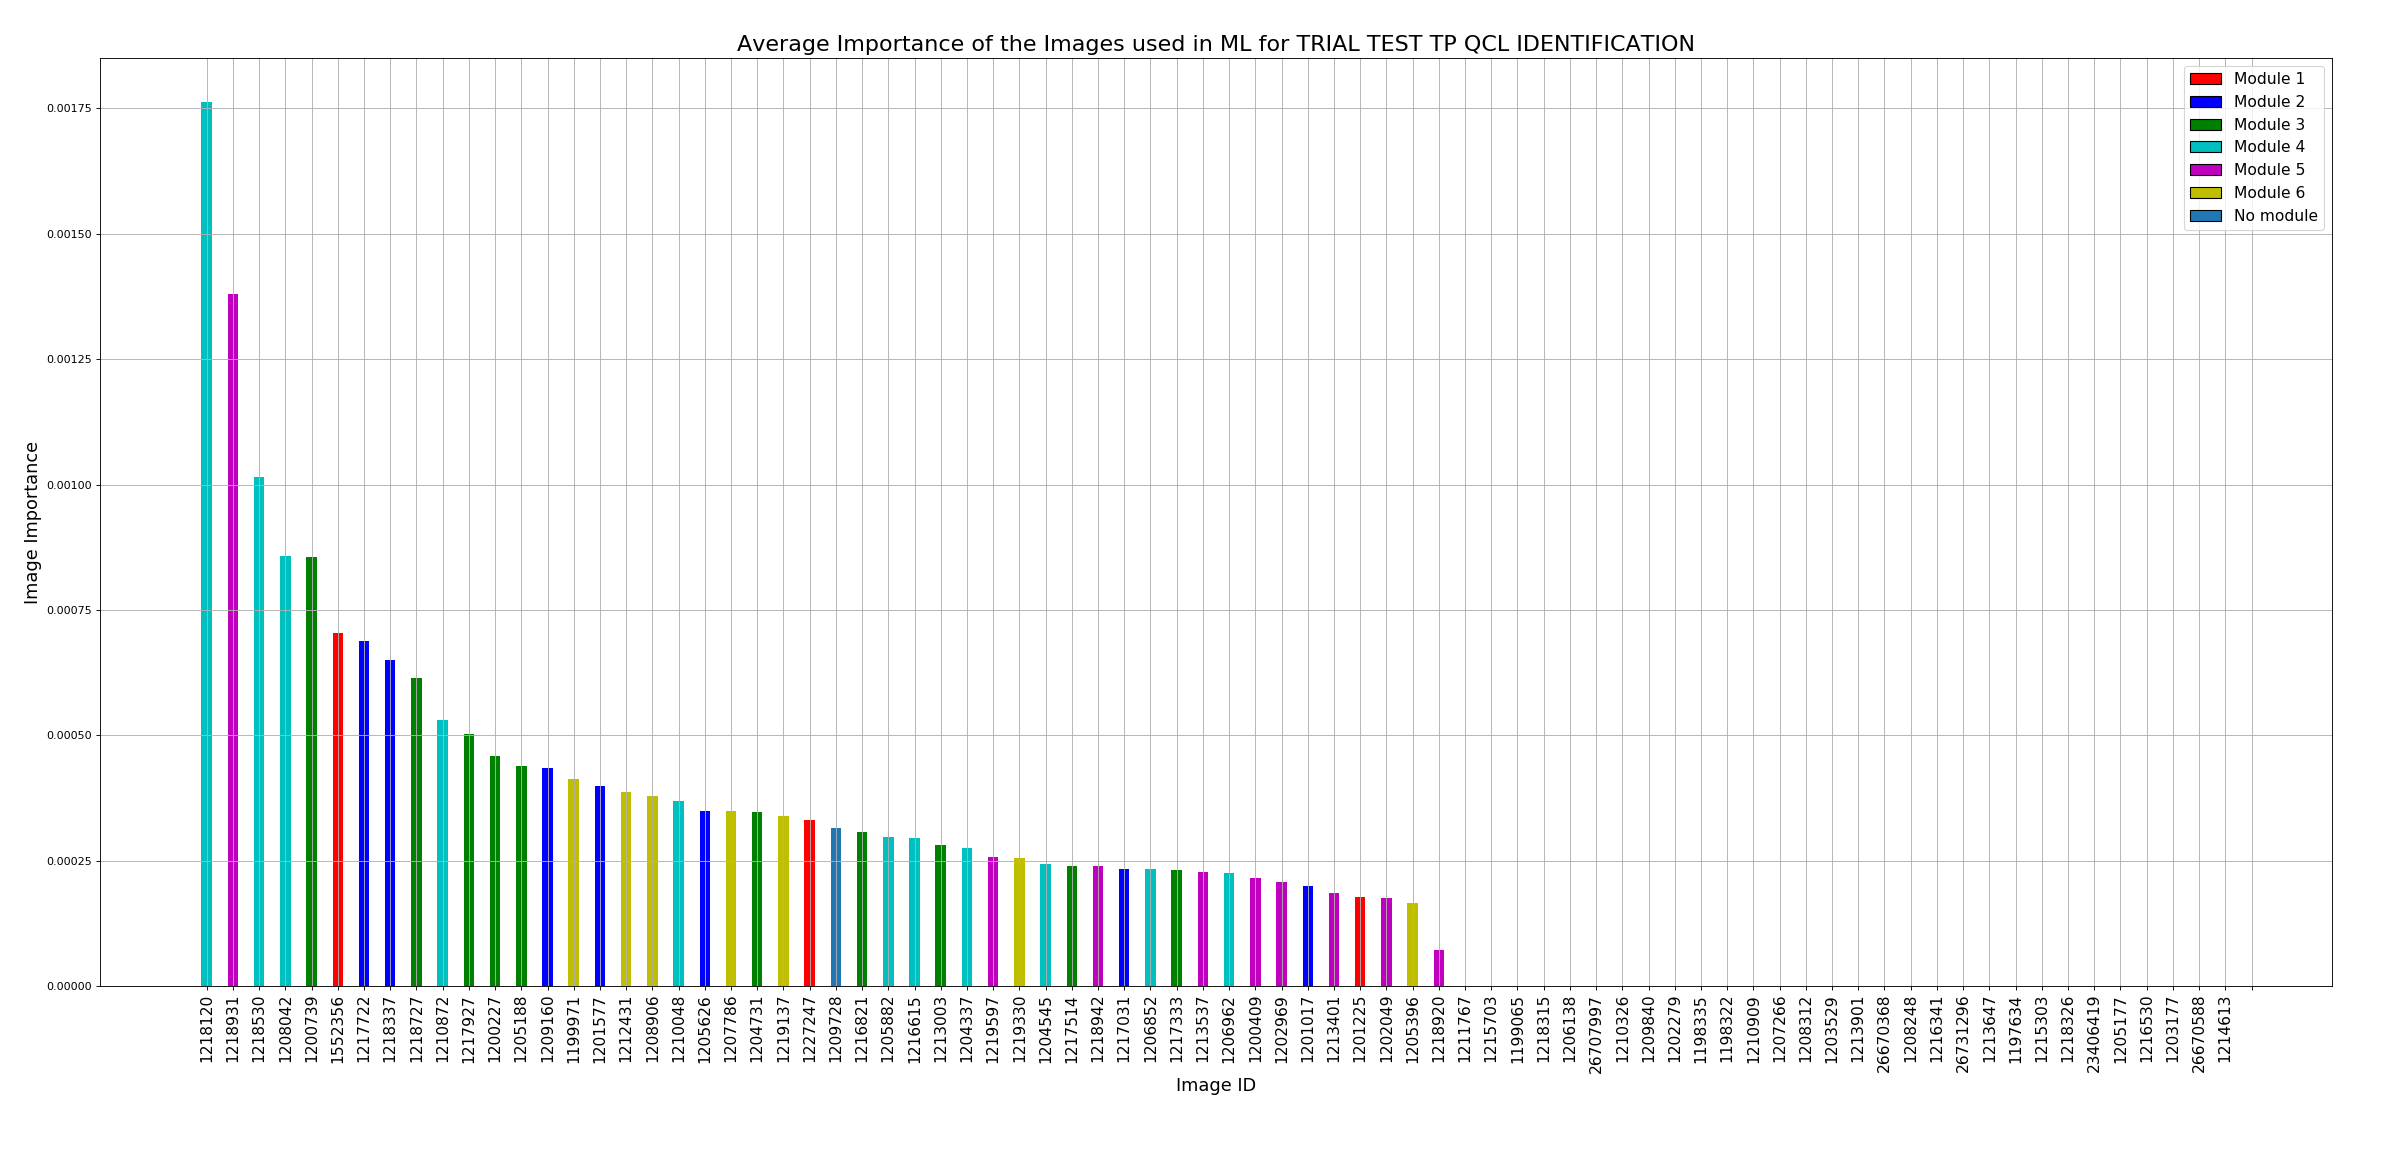
\includegraphics[width=.95\linewidth]{im_importance_TRIAL_TEST_TP_QCL_IDENTIFICATION_2018-04-29_14_28_06.png}
      \caption{Image Importance for the QCL Identification}
      \label{fig:im_white2}
      \end{figure}
      
      \begin{figure}[H]
      \centering
      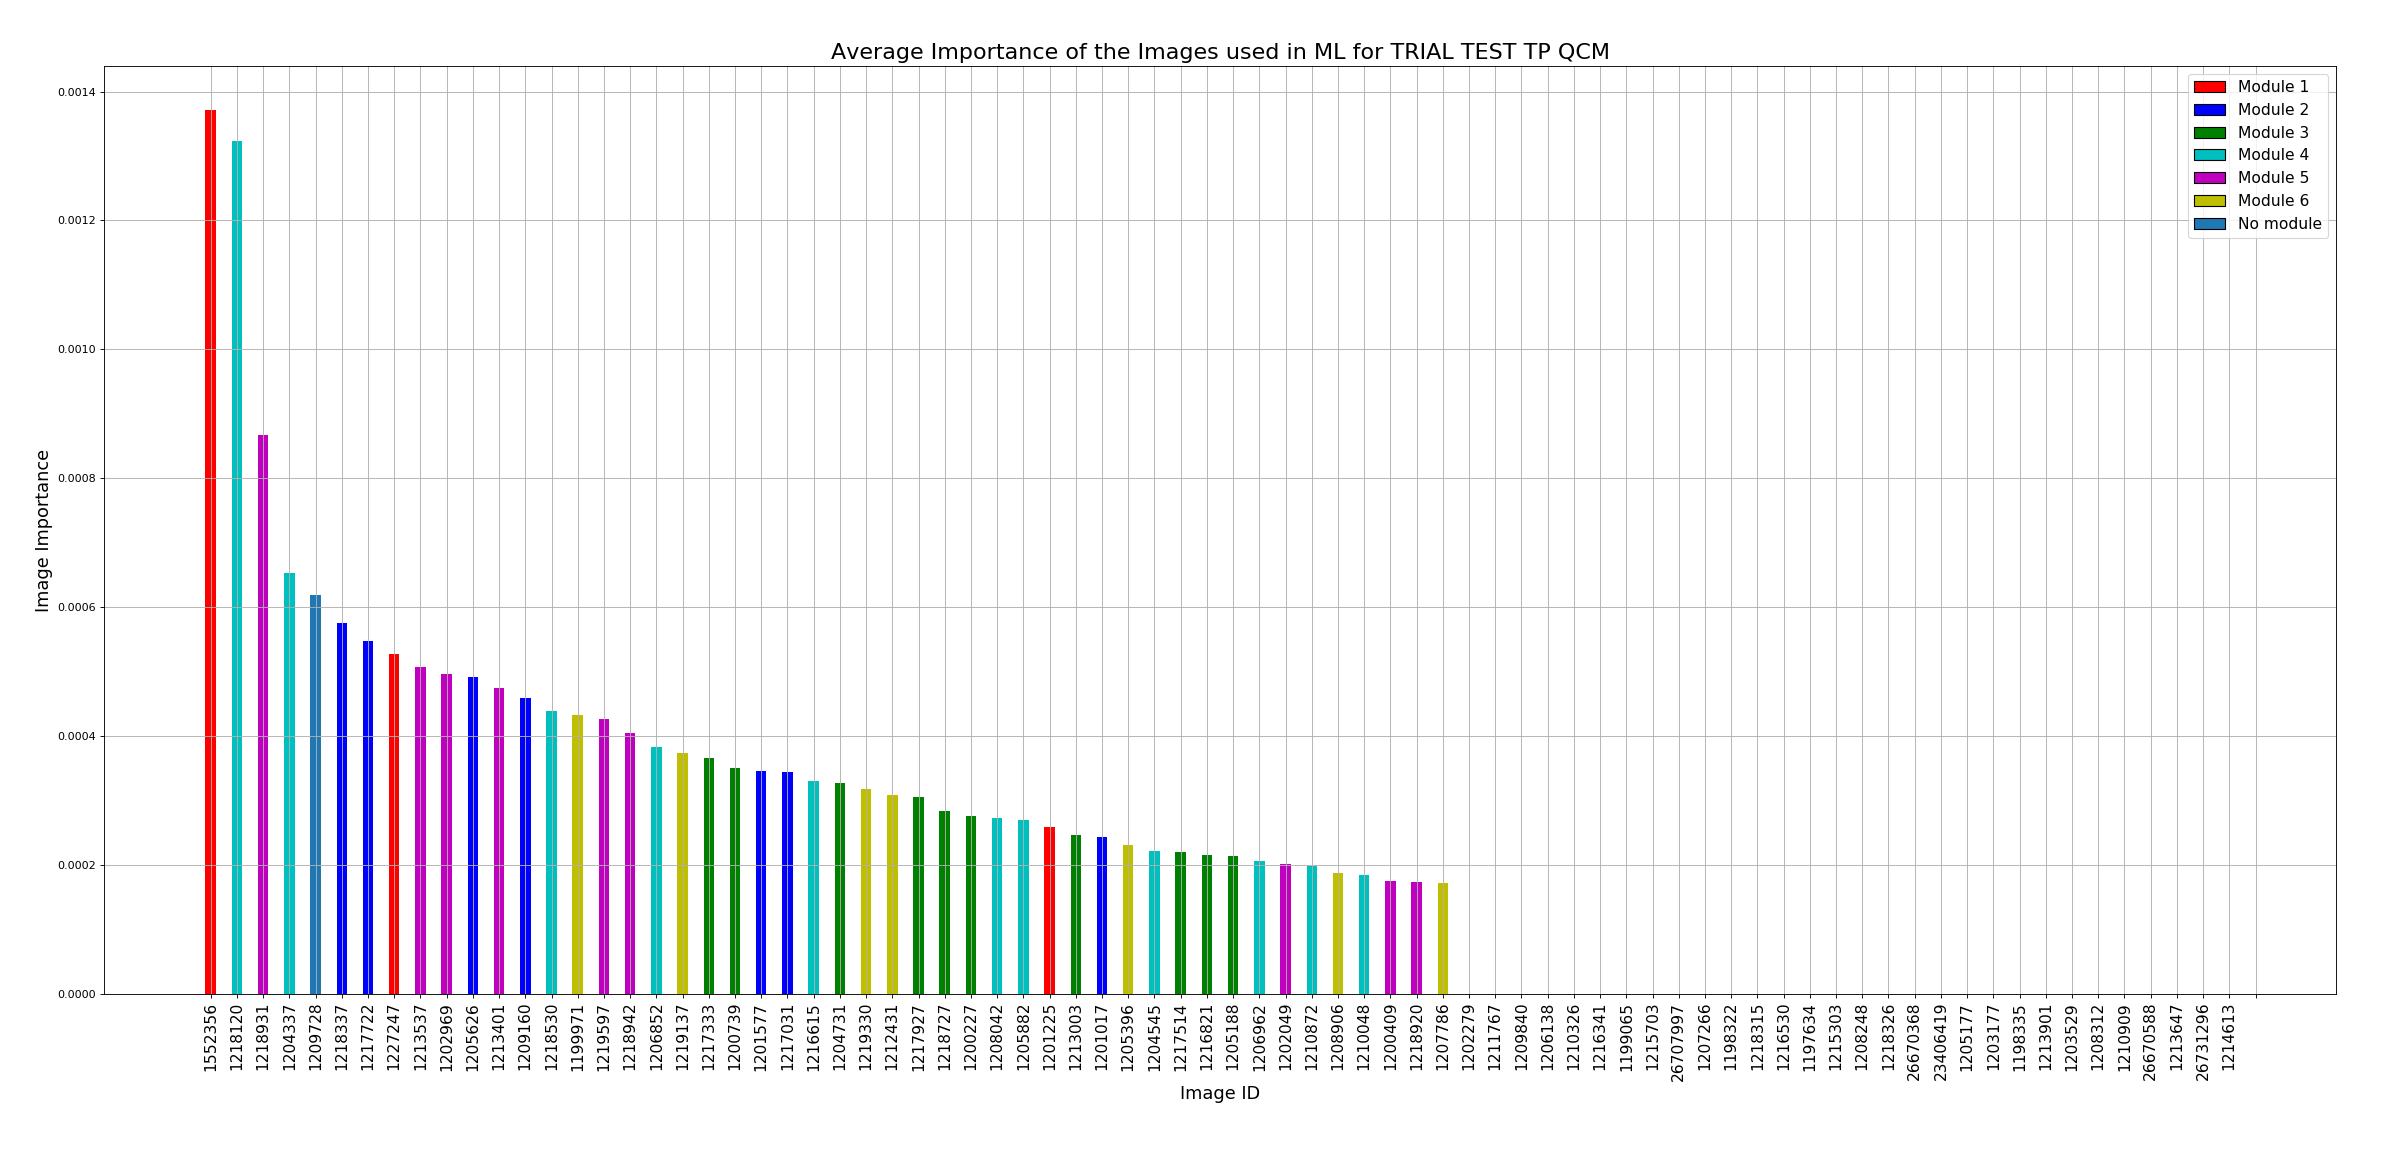
\includegraphics[width=.95\linewidth]{im_importance_TRIAL_TEST_TP_QCM_2018-04-29_14_34_19.png}
      \caption{Image Importance for the QCM}
      \label{fig:im_white3}
      \end{figure}
    
    As a reminder, out of all the images in the GOLD project, about a third of the images were not even visited.
    Also, some of the images don't belong to any module.
    It seems that as a general consensus that the most impactful images do not belong to the last module.
    This is due to the fact that the module 6 is not included in the trial exam.
    It's also worth noting that the module 1 is not included in the exam either.
    But since the module 1 is considered a tutorial, it can be useful.
    An image that appears often at the top is the image 1218120.
    This image was used for a preparation identification exercise.
    It seems that those who perform better in regards to that image on Cytomine do better in the white tests.
    For the QCL identification, the exercise images are often the most important over all the images in the same module.
    This seems to prove that doing the exercises seriously and correctly can lead to better grades.
    For the QCM, the image 1552356 which is a module 1 tutorial image is the most impactful.
    Those who follow the tutorial may have an easier time understanding the course from the start and may perform better for the QCM. As for the incidence test, the module 3 variables seem to be the most impactful.
    This module may contain examples that allow the student to better differentiate different incidence angles for specific objects in the images.
    OF course the cross validation results are not the best, so these assumption are not necessary correct. This leads to the actual practical exam.
    
    \subsubsection{Practical Exam Grades}

	There are a total of 5 practical exam results including the total.
	These \textbf{Y} variables tested similarly to the white tests.
	The exam took place on the 12th of June 2017.
	Unlike the white exam, the students should have finished working on all the modules.
	These exams also depend on the entirety of the program unlike
the white tests.
Since these exams are graded, students should have the motivation to study and apply themselves. (Figure \ref{fig:results_prac})

    \begin{figure}[H]
      \centering
      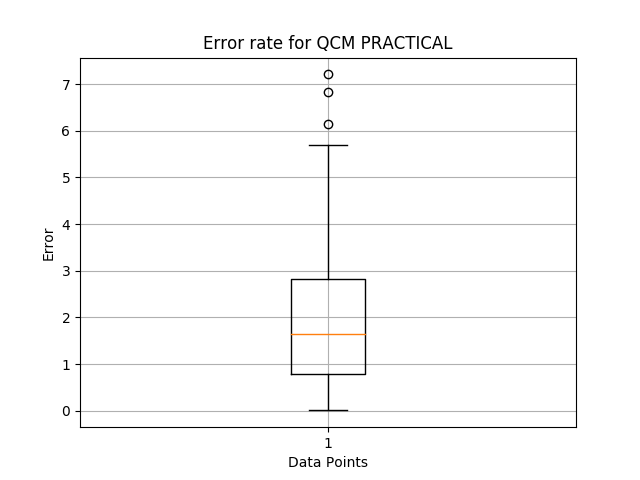
\includegraphics[width=.30\linewidth]{cv_boxplot_QCM_PRACTICAL_2018-04-27_19_12_27.png}
      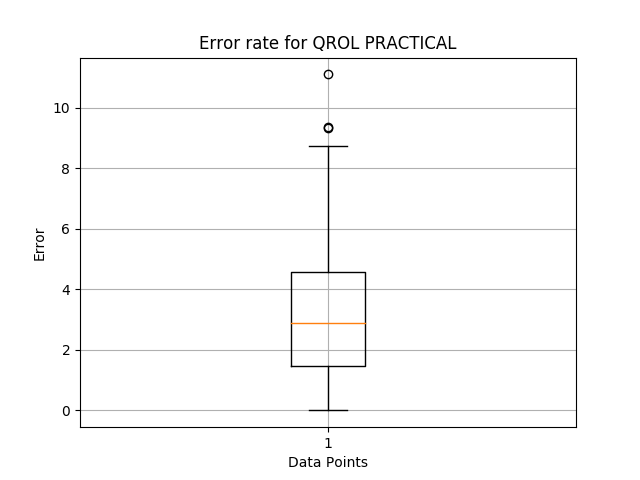
\includegraphics[width=.30\linewidth]{cv_boxplot_QROL_PRACTICAL_2018-04-27_19_11_08.png}\\
      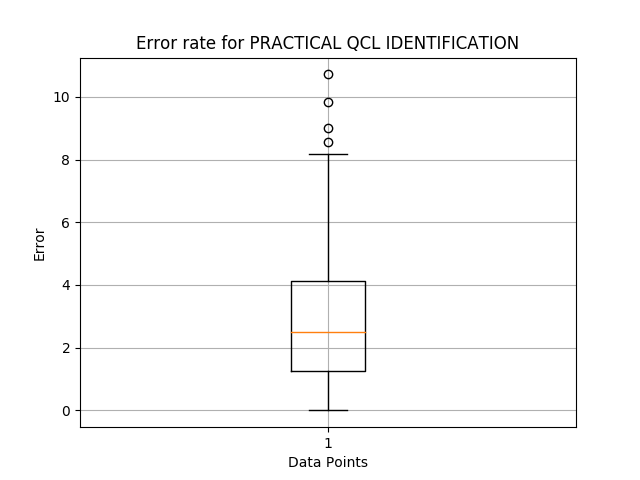
\includegraphics[width=.30\linewidth]{cv_boxplot_PRACTICAL_QCL_IDENTIFICATION_2018-04-27_16_59_01.png}
  	  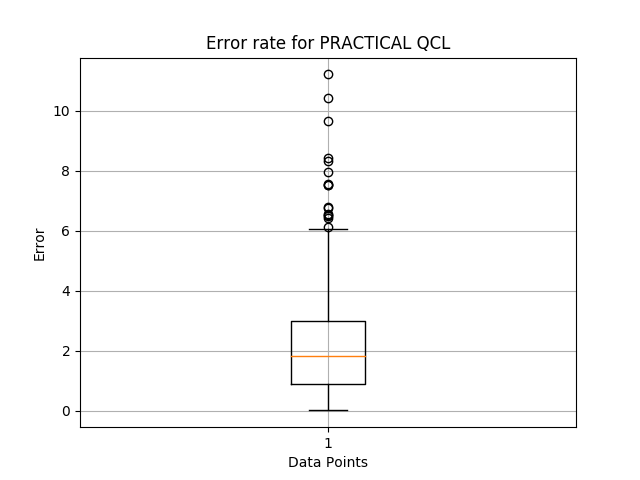
\includegraphics[width=.30\linewidth]{cv_boxplot_PRACTICAL_QCL_2018-04-27_17_10_02.png}
      \\
      \ref{fig:results_prac}.1: Boxplots of the error values
      \\
      \vspace{0.5cm}
      \begin{tabular}{| l | c | c | c | c | c |}
      \hline
      & \tiny{Score} & \tiny{Median Score} & \tiny{Score Difference} & \tiny{Real Median Grade} & \tiny{Median Est.
      Grade}\\ \hline
      \tiny{QCM practical} & \tiny{1.94} & \tiny{2.29} & \tiny{0.36} & \tiny{10.80} & \tiny{11.01}\\ \hline
      \tiny{QROL practical} & \tiny{3.23} & \tiny{3.64} & \tiny{0.40} & \tiny{7.93} & \tiny{8.80}\\ \hline
      \tiny{QCL identification Practical} & \tiny{2.86} & \tiny{3.36} & \tiny{0.5} & \tiny{11.0} & \tiny{11.61}\\ \hline
      \tiny{QCL incidence Practical} & \tiny{2.23} & \tiny{2.83} & \tiny{0.59} & \tiny{15.0} & \tiny{15.32}\\
      \hline
      \end{tabular}\\
      \vspace{0.5cm}
      \ref{fig:results_prac}.2: Discrete Results\\
      \vspace{0.3cm}
      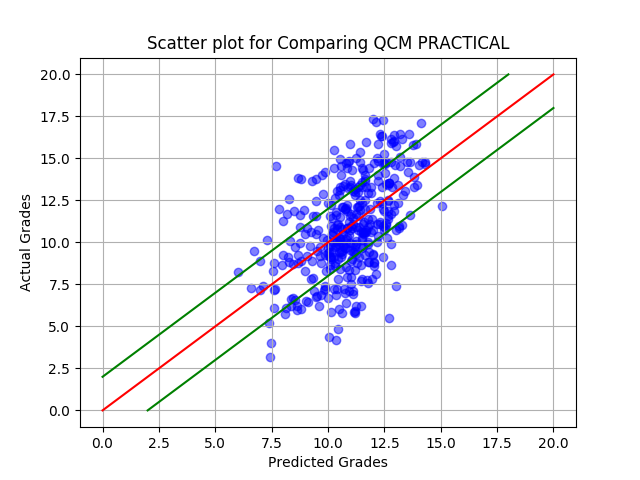
\includegraphics[width=.30\linewidth]{cv_comp_QCM_PRACTICAL_2018-04-27_19_12_27.png}
      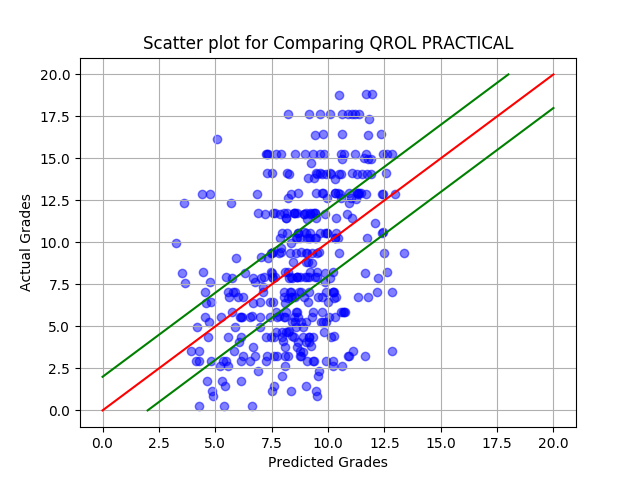
\includegraphics[width=.30\linewidth]{cv_comp_QROL_PRACTICAL_2018-04-27_19_11_08.png}\\
      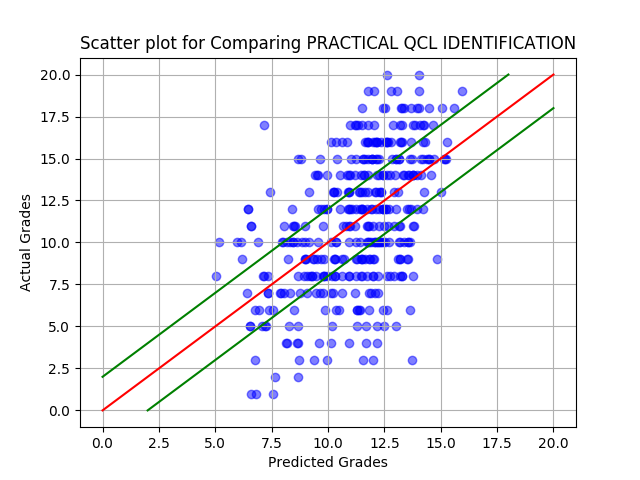
\includegraphics[width=.30\linewidth]{cv_comp_PRACTICAL_QCL_IDENTIFICATION_2018-04-27_16_59_01.png}
  	  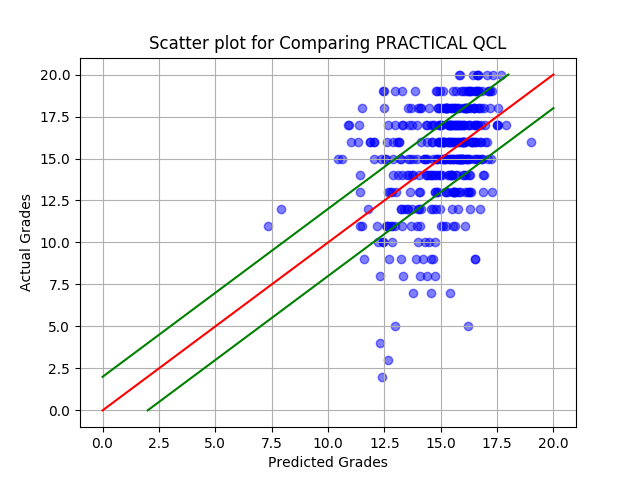
\includegraphics[width=.30\linewidth]{cv_comp_PRACTICAL_QCL_2018-04-27_17_10_02.png}
      \\
      \ref{fig:results_prac}.3: Actual grades compared to Predicated grades
      \caption{Results from cross-validation of the White Tests}
      \label{fig:results_prac}
    \end{figure}

	the results obtained are more interesting.
	The results vary heavily depending on the exams that were taken.
	All the scores are significantly better than their respective median compared to the trial tests.
    \begin{itemize}
    \item[\textbullet]  QCM practical : The best score, the boxplots show the most well rounded results.
    The 75 percentile of grades estimated have an error of less than 3 and a 25 percentile of grades with an error of less than 1.
    Unfortunately, there are still some cases with a significantly high error.
    As for relation between the expected grade and the estimated grade, there is a clear pattern following the red line.
    The exception being that low actual grades are overestimated by the model.
    QCM exams are usually are straight to the point.
    Students need to know the answer to question but they don't have to explain it.
    All students by definition are graded equally because the exam is straightforward and easy to correct.
    \item[\textbullet]  QROL practical : As opposed to the QCM, the score is significantly worse.
    This is also shown by the boxplot where the 75 percentile is at less than 4.5. By comparing the grades, it's apparent that there are more extreme grades and their estimations are off for the most part.
    This is normal because students write long and detailed responses to the questions.
    The teachers are more critical of the students.
    They look to see if students understand the contents of the course as opposed to learning by heart.
    \item[\textbullet]  QCL identification Practical : With a score of 2.86, this QCL does not offer the best results.
    It follows a somewhat lessened pattern of the QROL. As this portion of the exam gives the student an exhaustive list of possible answers, it's hard to a student to guess.
    It's critical that the students knows what they observe.
    Similarly to the QROL, lack of certainty lowers the grade.
    As opposed to the QCM where uncertainty is not much of an issue due to the lack of options.
    \item[\textbullet]  QCL incidence Practical : the incidence score  is somewhat better.
    Apart from a couple exceptions most of the real grades have a small variance.
    This helps explain the very low 75 percentile of about 3 and the big number of erroneous cases above 6.
    Since this part of the exam is similar to a QCM but with only 3 options, it's relatively easy to answer the questions correctly.
    This explains the higher grades for most students.
    \end{itemize}
    
    When taking practical exams the students have images to look at.
    Certain aspects of the images need to be identified before answering the questions.
    Unfortunately with the data fetched from Cytomine, it's hard to determine whether or not the students were able to identify certain concepts when using Cytomine.
    But attempting to identify the features that are close to determining whether or not a student understood the course is a start. (Figures \ref{fig:var_tp1}, \ref{fig:var_tp2}, \ref{fig:var_tp3},\ref{fig:var_tp4})

     \begin{figure}[H]
      \centering
      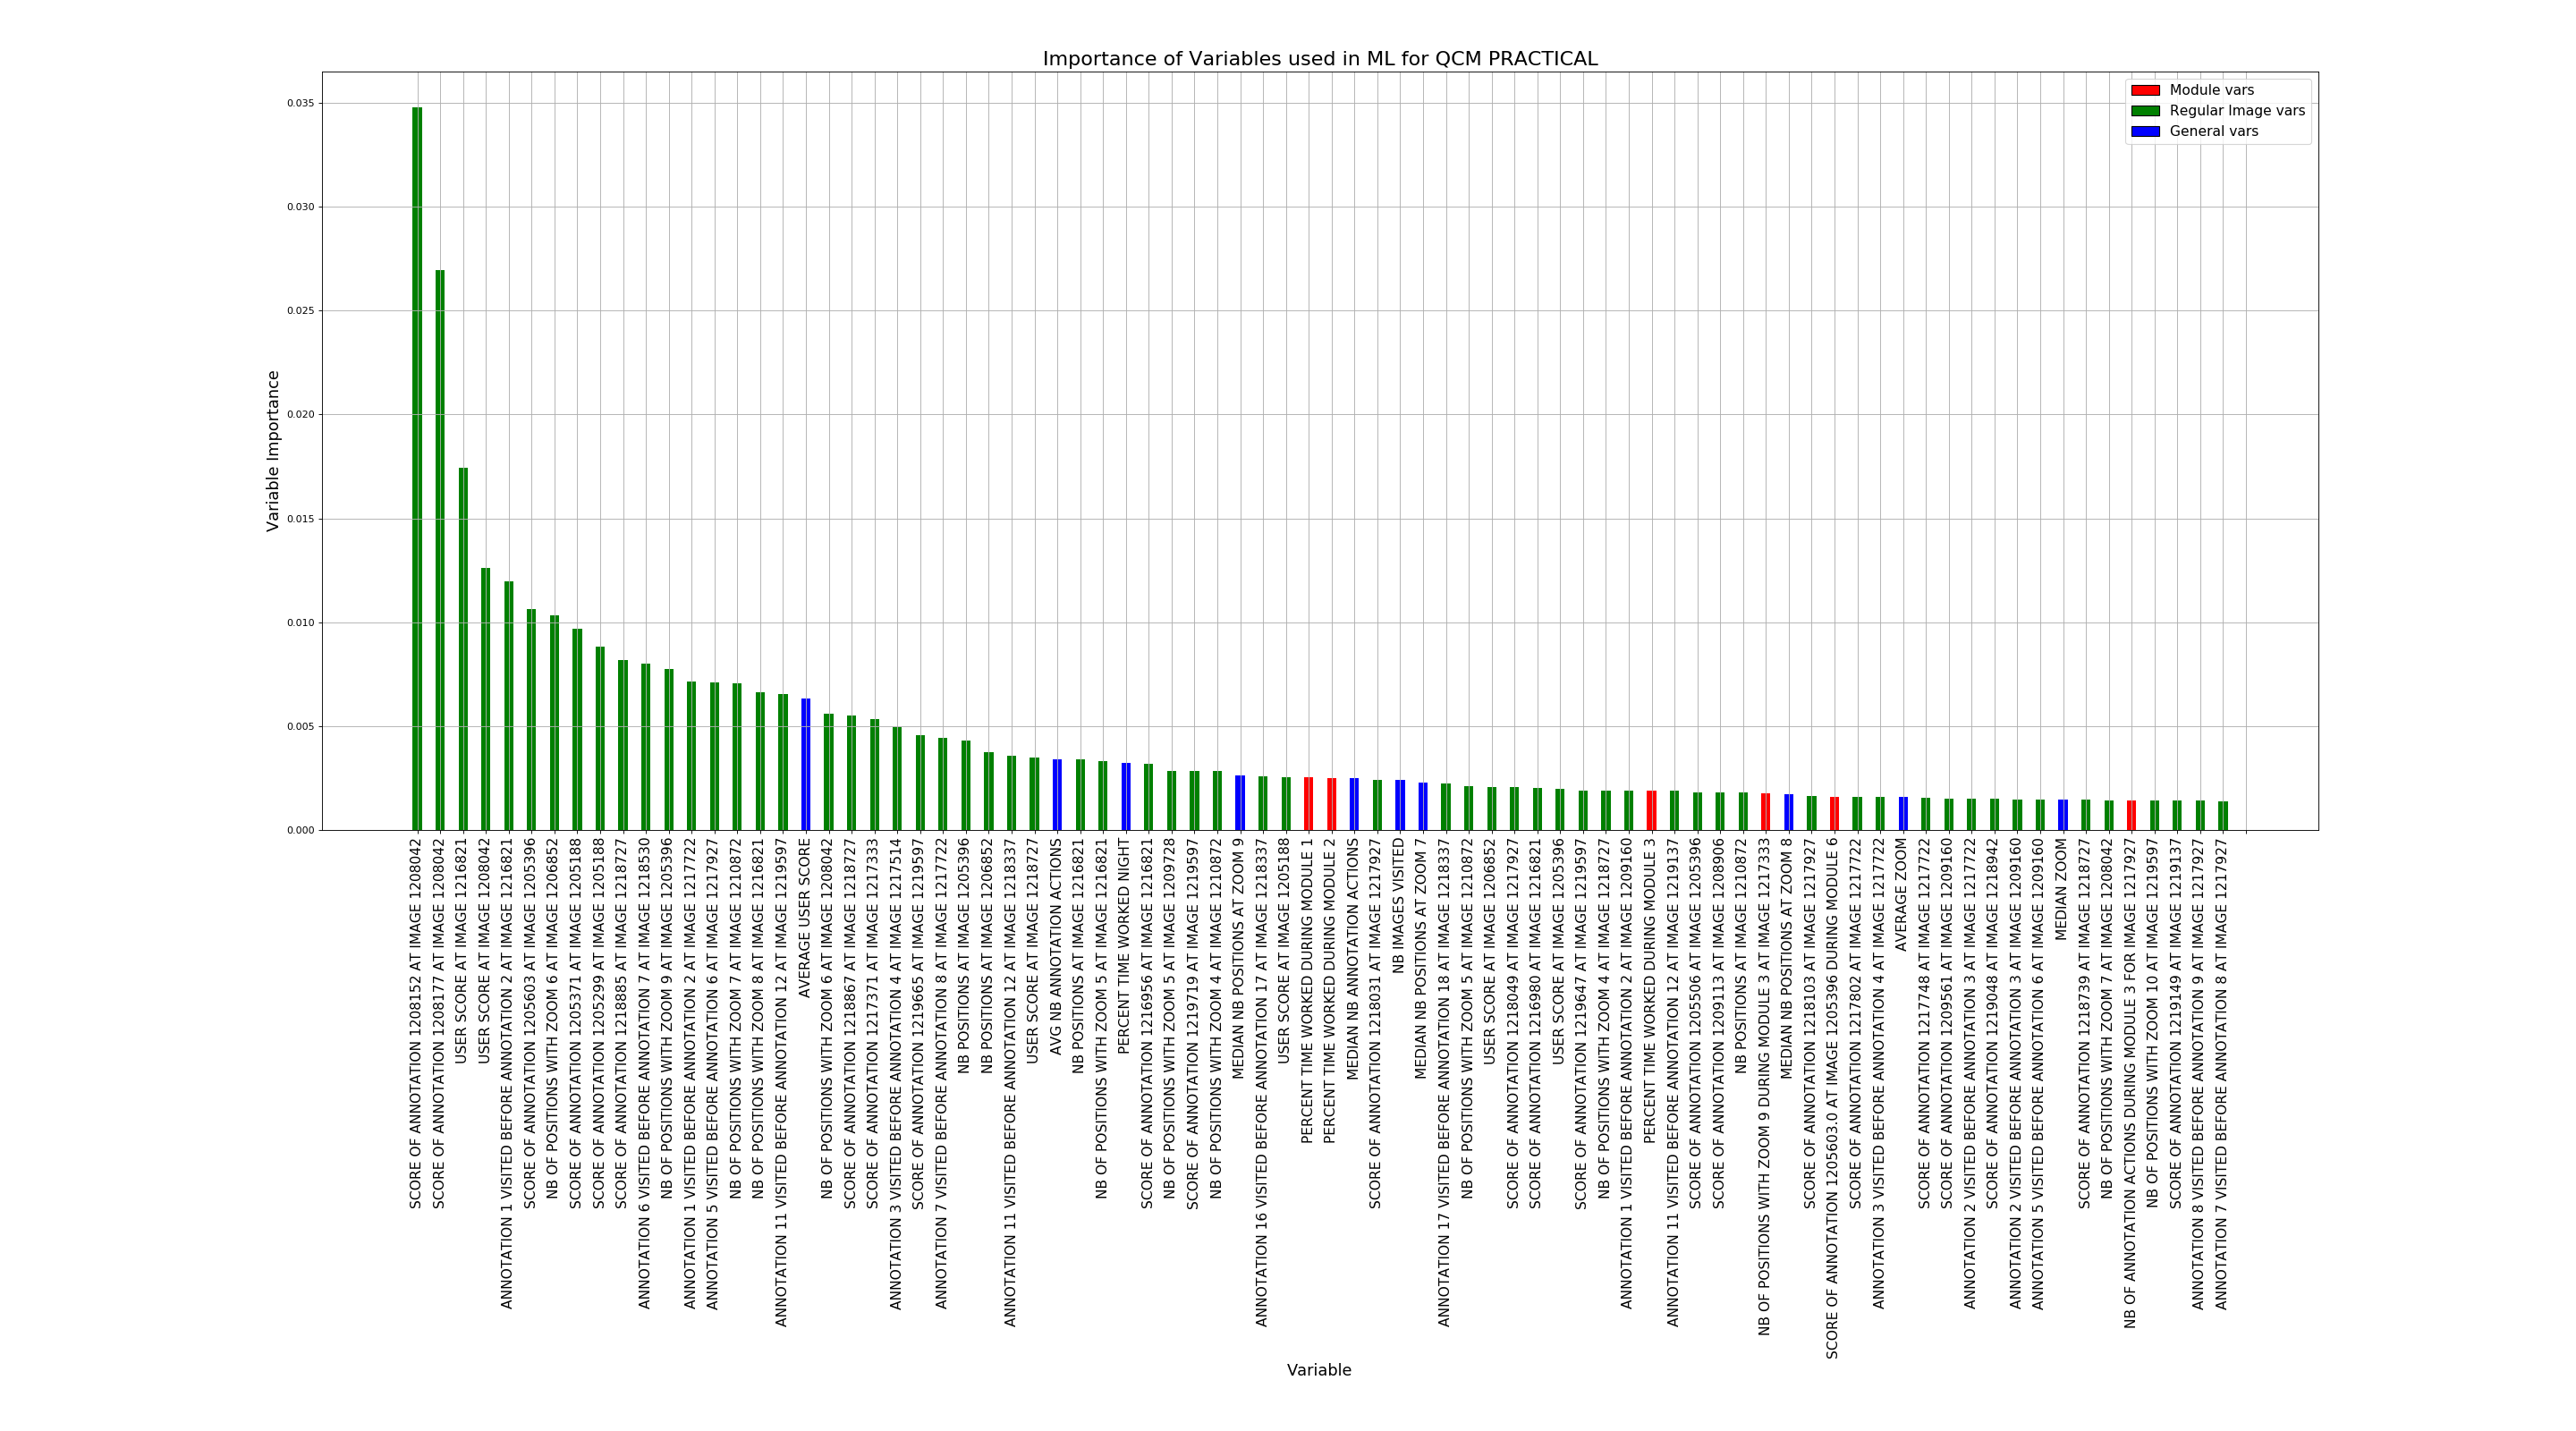
\includegraphics[width=.95\linewidth]{var_importance_QCM_PRACTICAL_2018-04-29_14_38_13.png}
      \caption{Feature Importance for the QCM Practical}
      \label{fig:var_tp1}
      \end{figure}
      
      \begin{figure}[H]
      \centering
      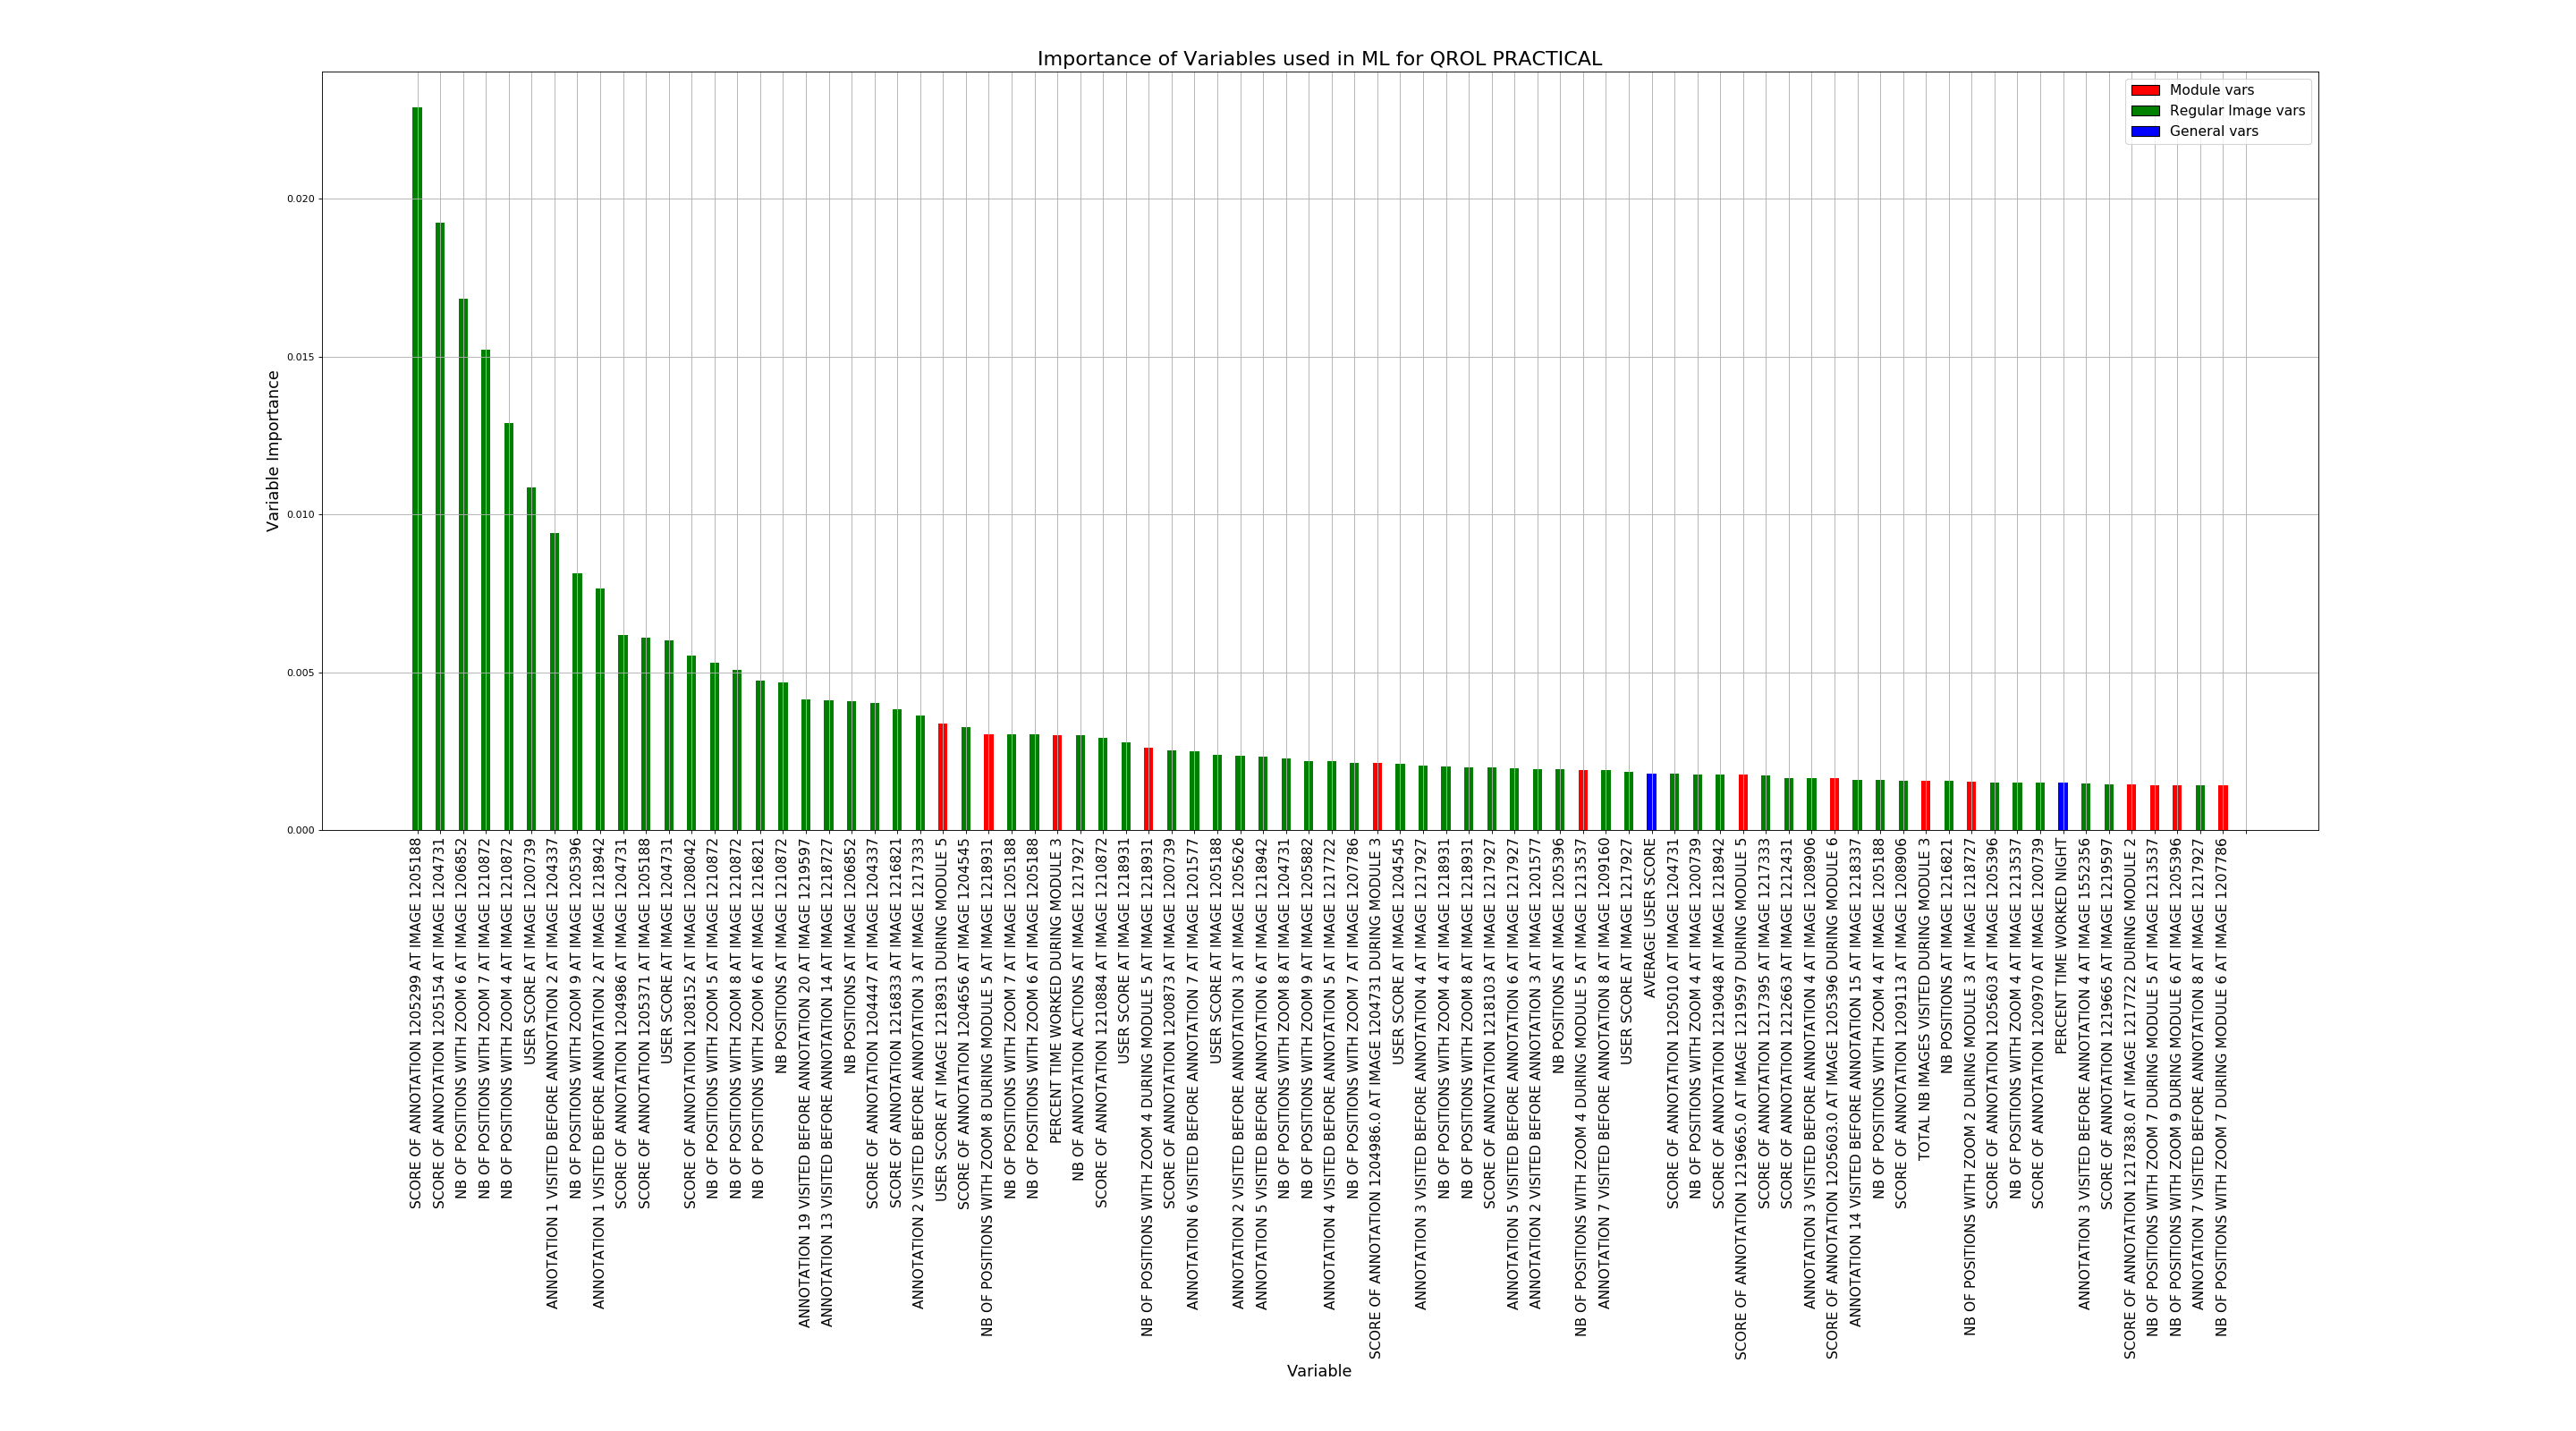
\includegraphics[width=.95\linewidth]{var_importance_QROL_PRACTICAL_2018-04-29_14_37_04.png}
      \caption{Feature Importance for the QROL Practical}
      \label{fig:var_tp2}
      \end{figure}
      
      \begin{figure}[H]
      \centering
      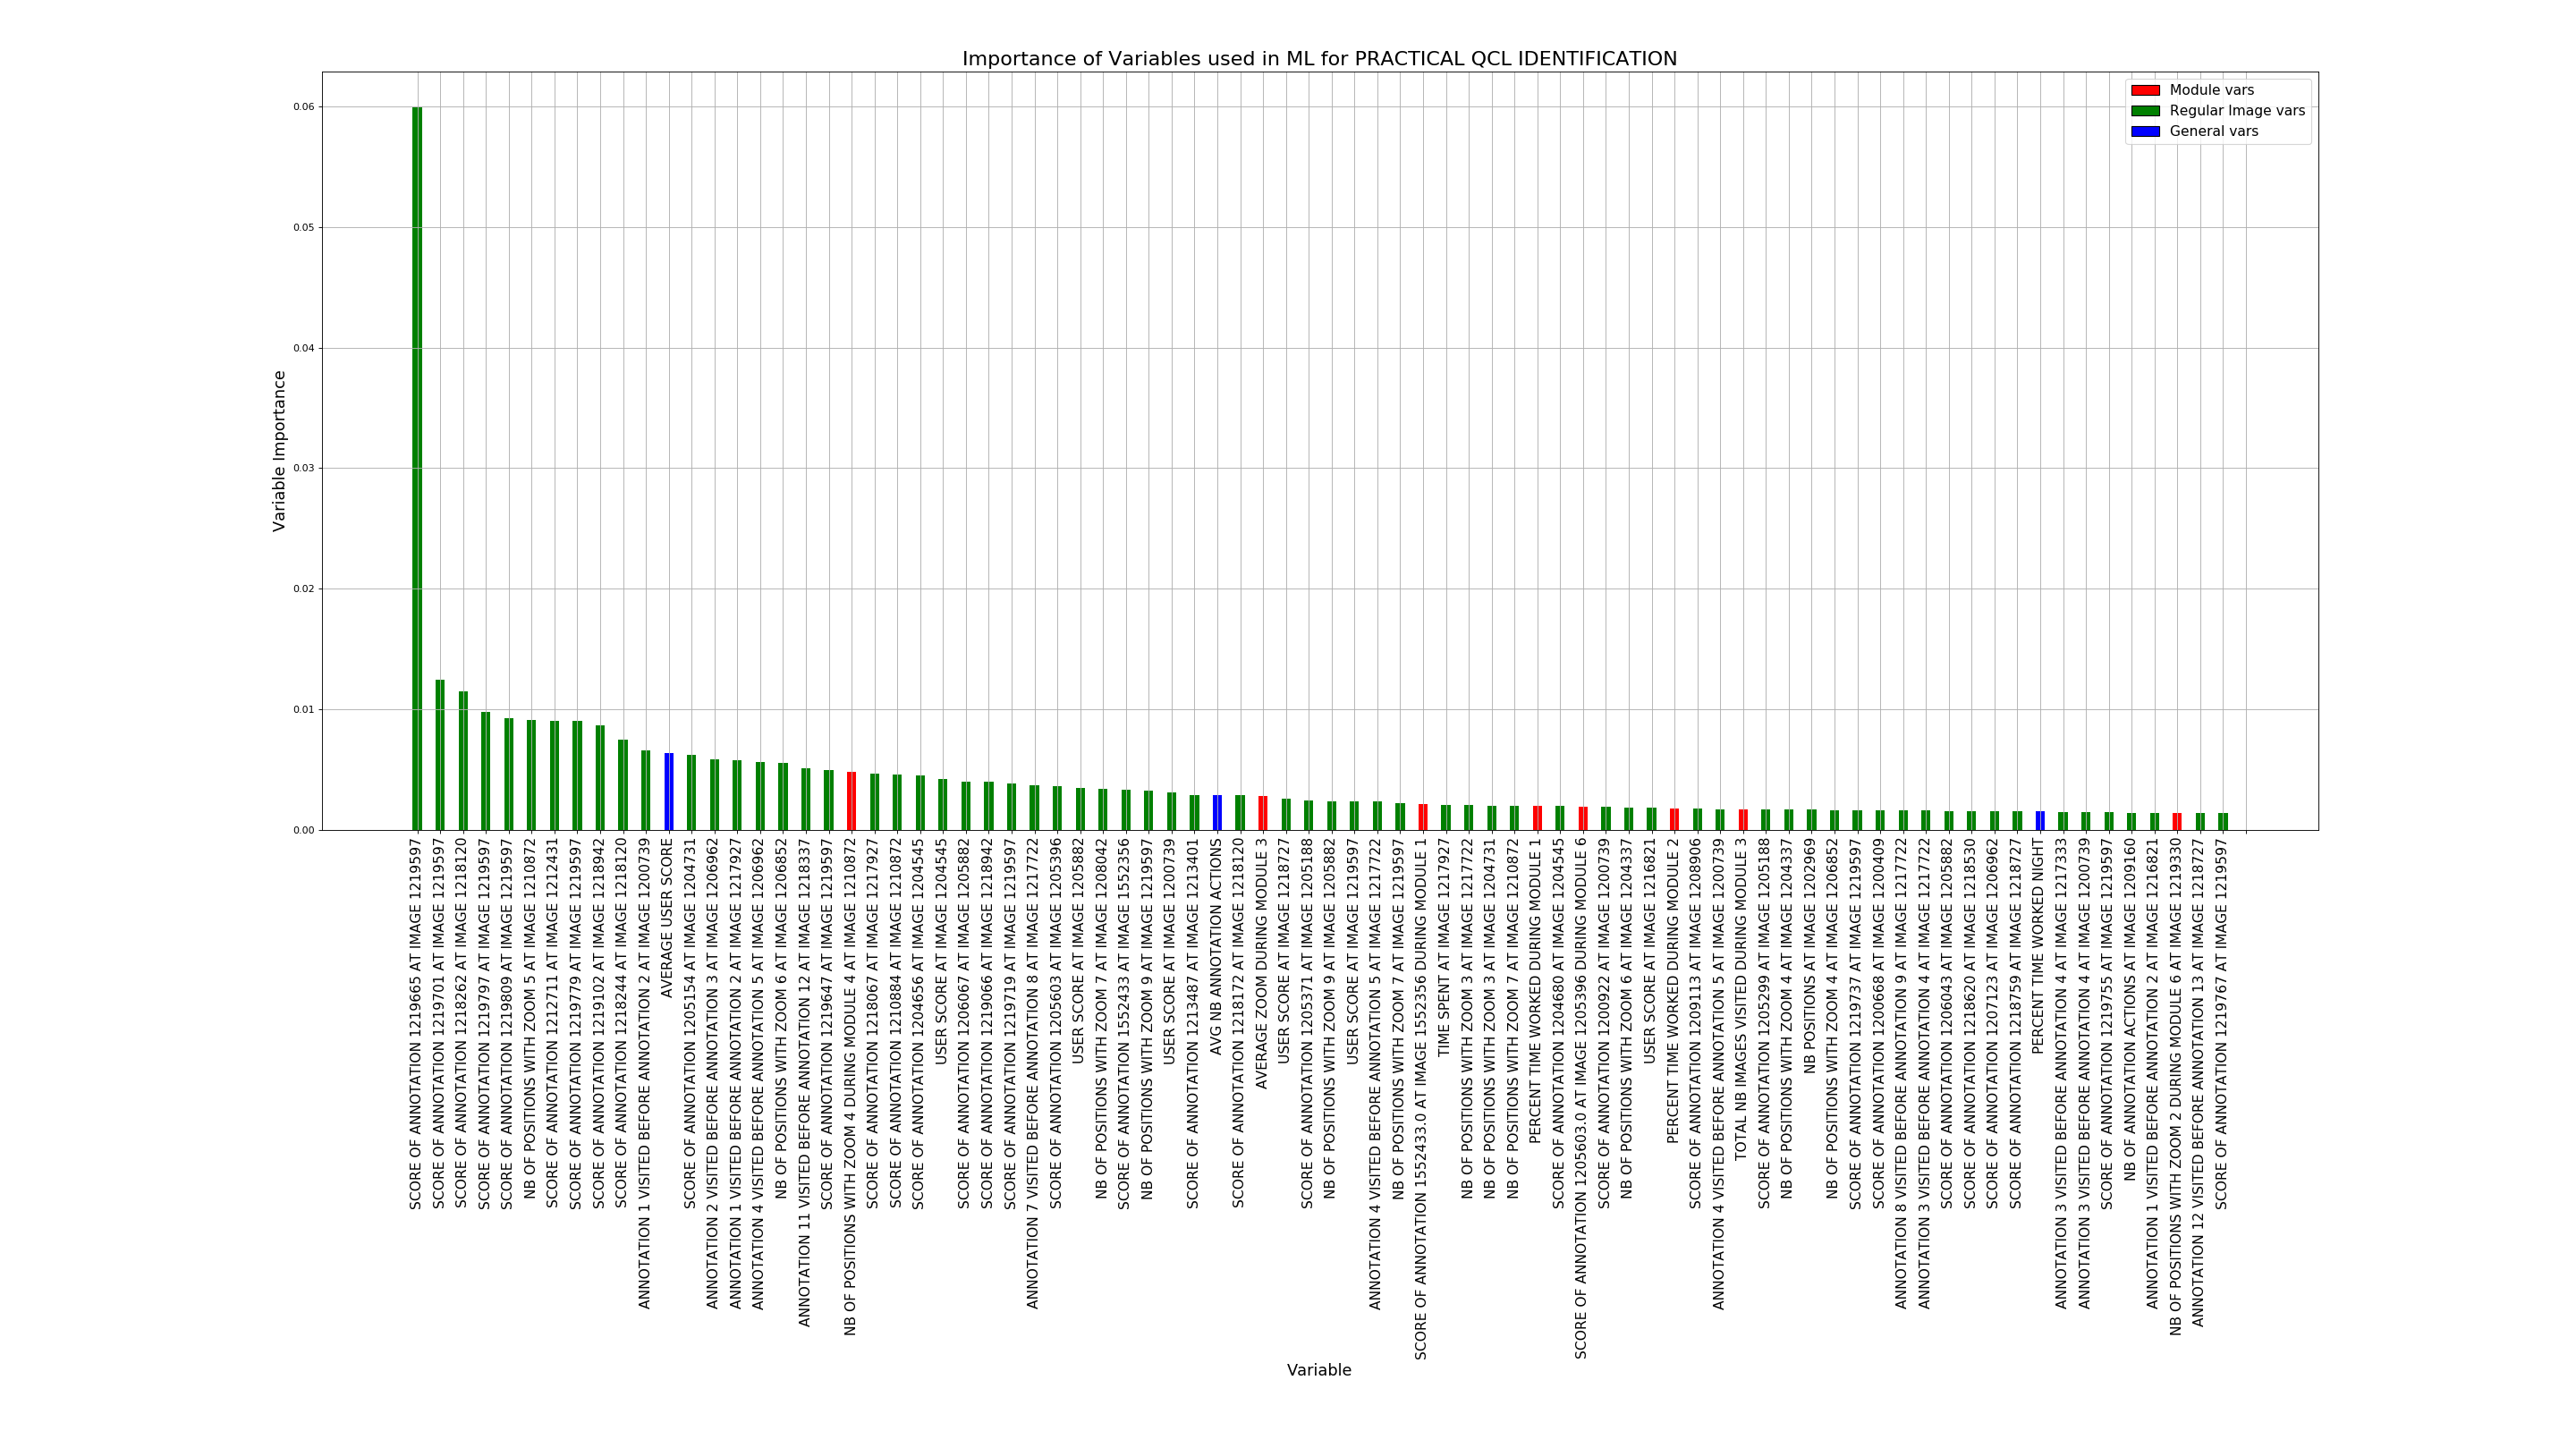
\includegraphics[width=.95\linewidth]{var_importance_PRACTICAL_QCL_IDENTIFICATION_2018-04-29_14_34_11.png}
      \caption{Feature Importance for the QCL Identification}
      \label{fig:var_tp3}
      \end{figure}
      
      \begin{figure}[H]
      \centering
      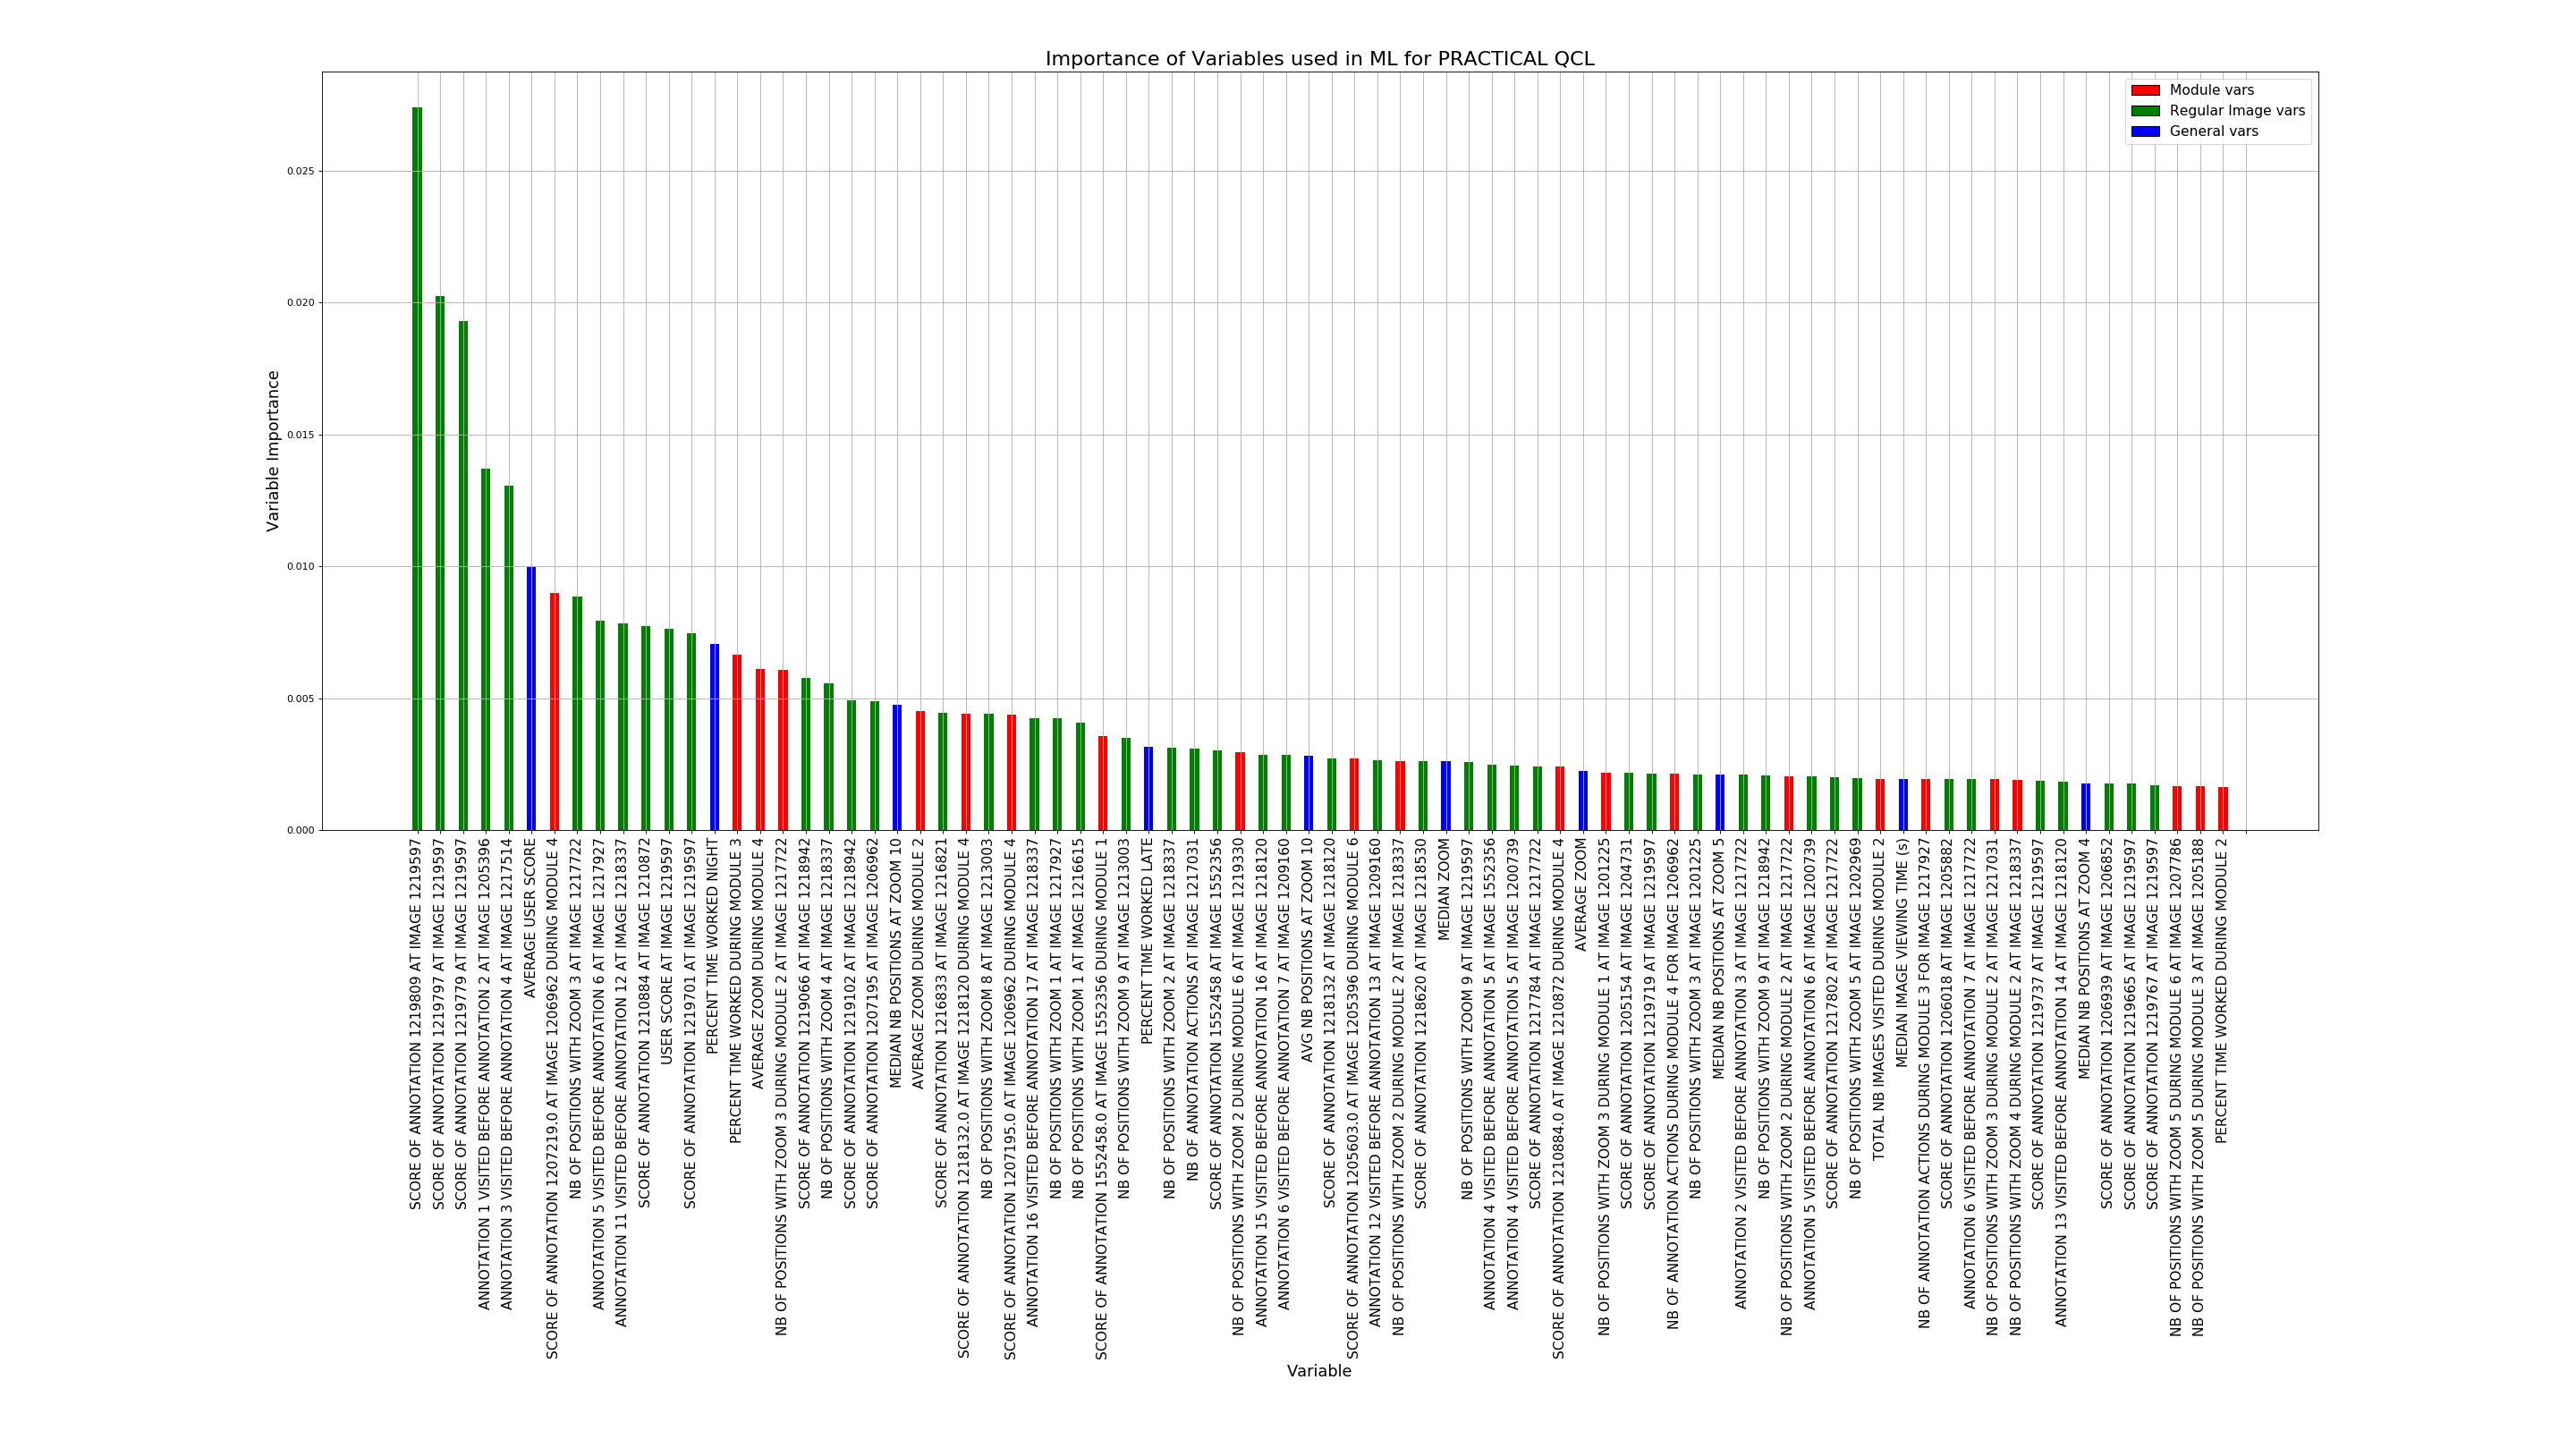
\includegraphics[width=.95\linewidth]{var_importance_PRACTICAL_QCL_2018-04-29_14_33_44.png}
      \caption{Feature Importance for the QCL Incidence}
      \label{fig:var_tp4}
      \end{figure}

The results are different from the trial tests.
For one, the Module features are relatively less impactful than before.
This shows that the total work done throughout the semester is more important than working more during specific modules.
It also is shown that the students spent the most time on Cytomine the day before the exam.%%todo add reference to timeline
Similar to the white tests models, the Average Score feature always shows up as an important feature.
This variable seems to be the closest variable into determining whether or not a student understands the course but it's still not perfect.
In the end, some images and some modules have more impact than others.  (Figures \ref{fig:im_tp1}, \ref{fig:im_tp2}, \ref{fig:im_tp3},\ref{fig:im_tp4})

     \begin{figure}[H]
      \centering
      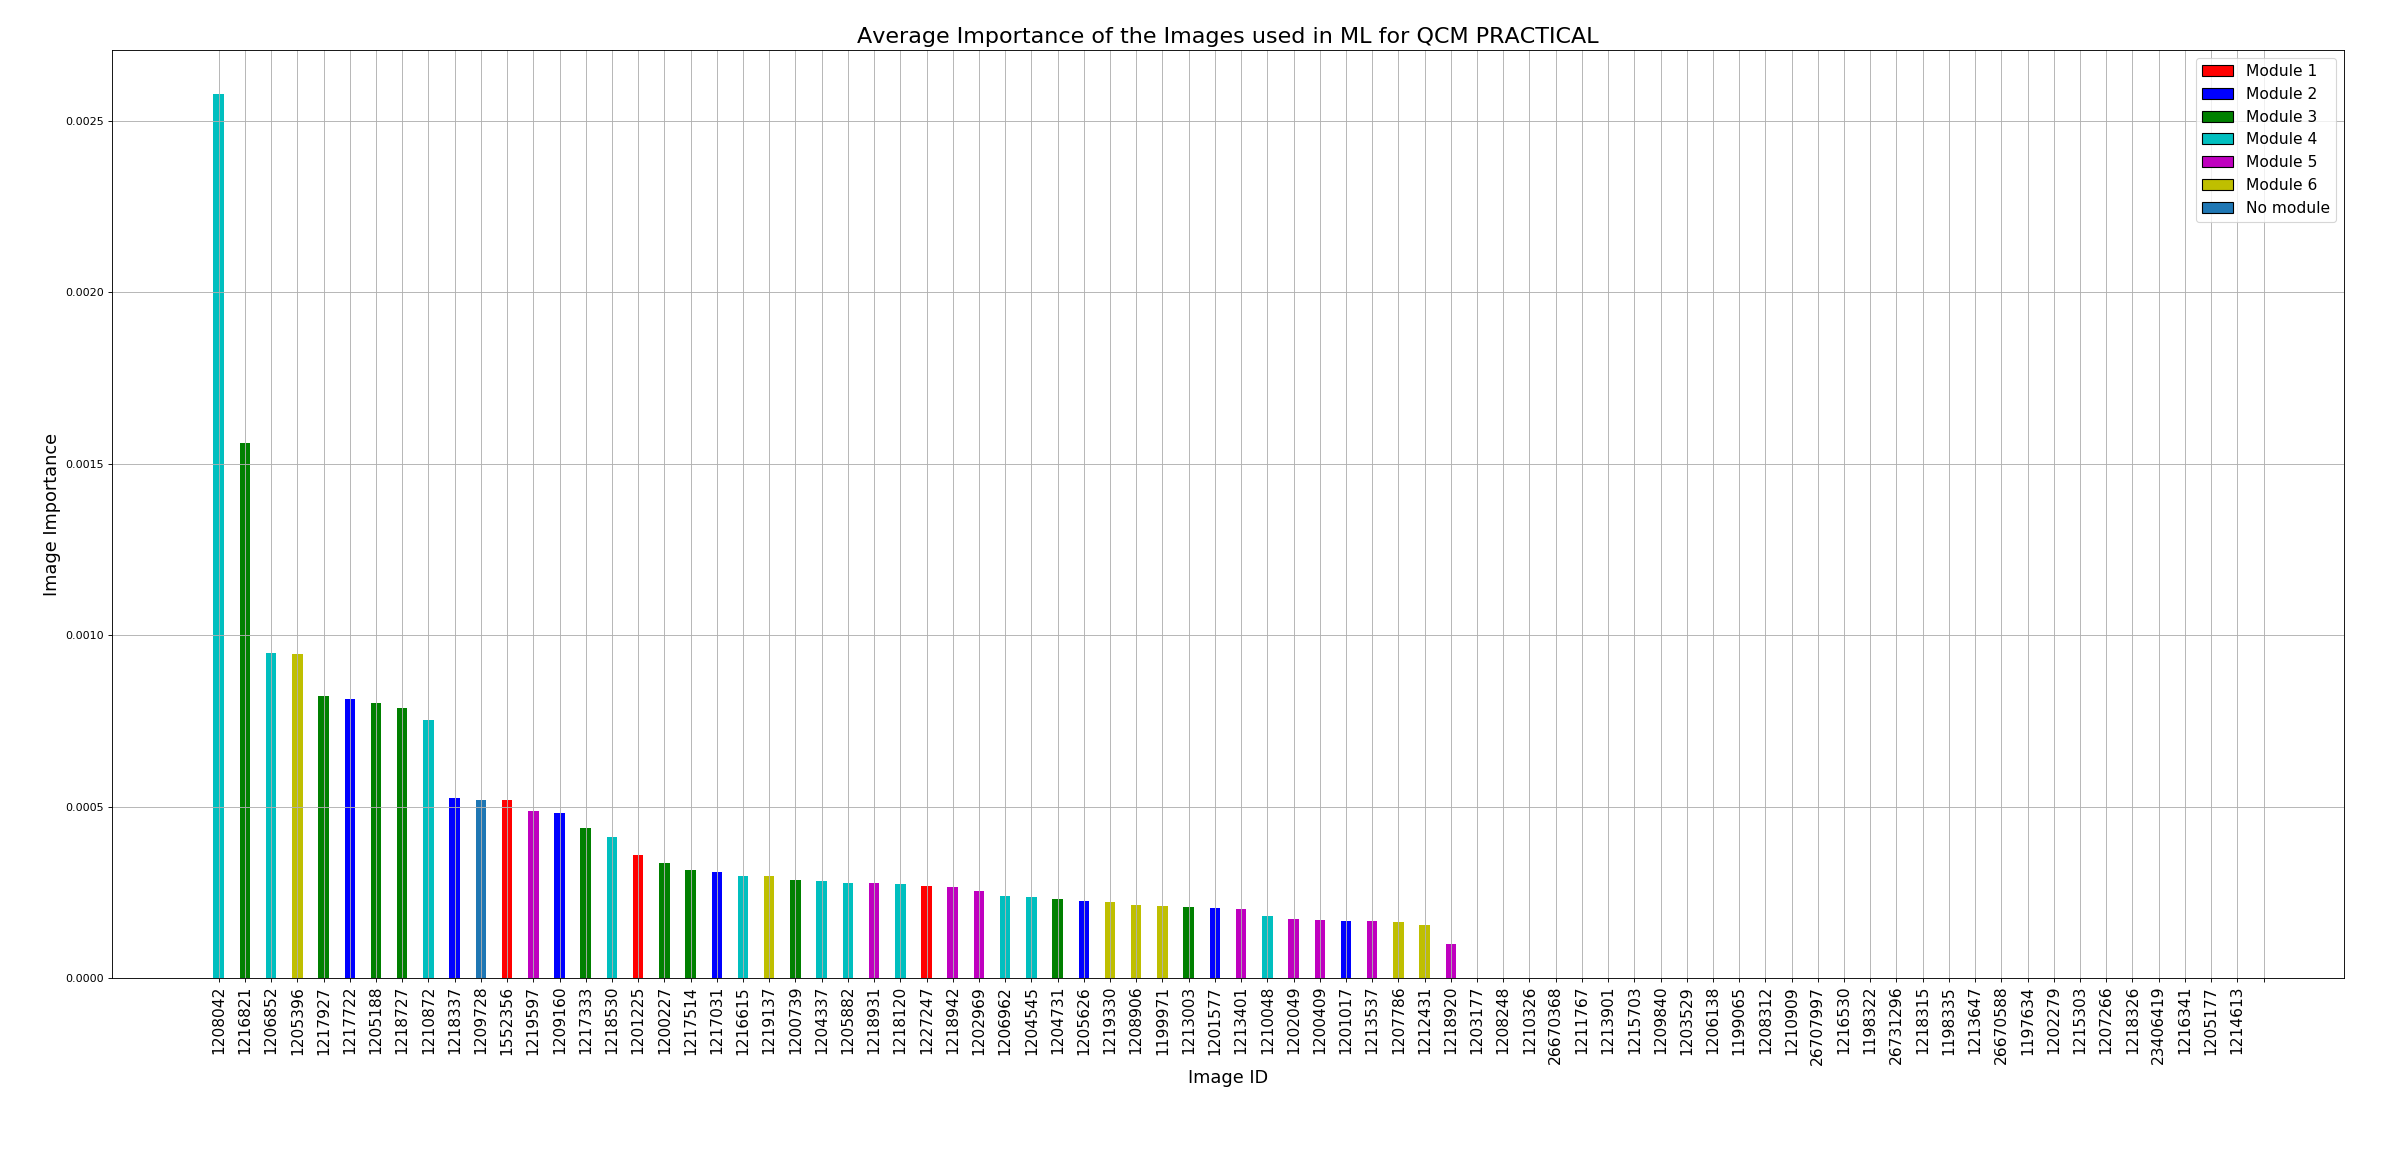
\includegraphics[width=.95\linewidth]{im_importance_QCM_PRACTICAL_2018-04-29_14_38_16.png}
      \caption{Image Importance for the QCM Practical}
      \label{fig:im_tp1}
      \end{figure}
      
      \begin{figure}[H]
      \centering
      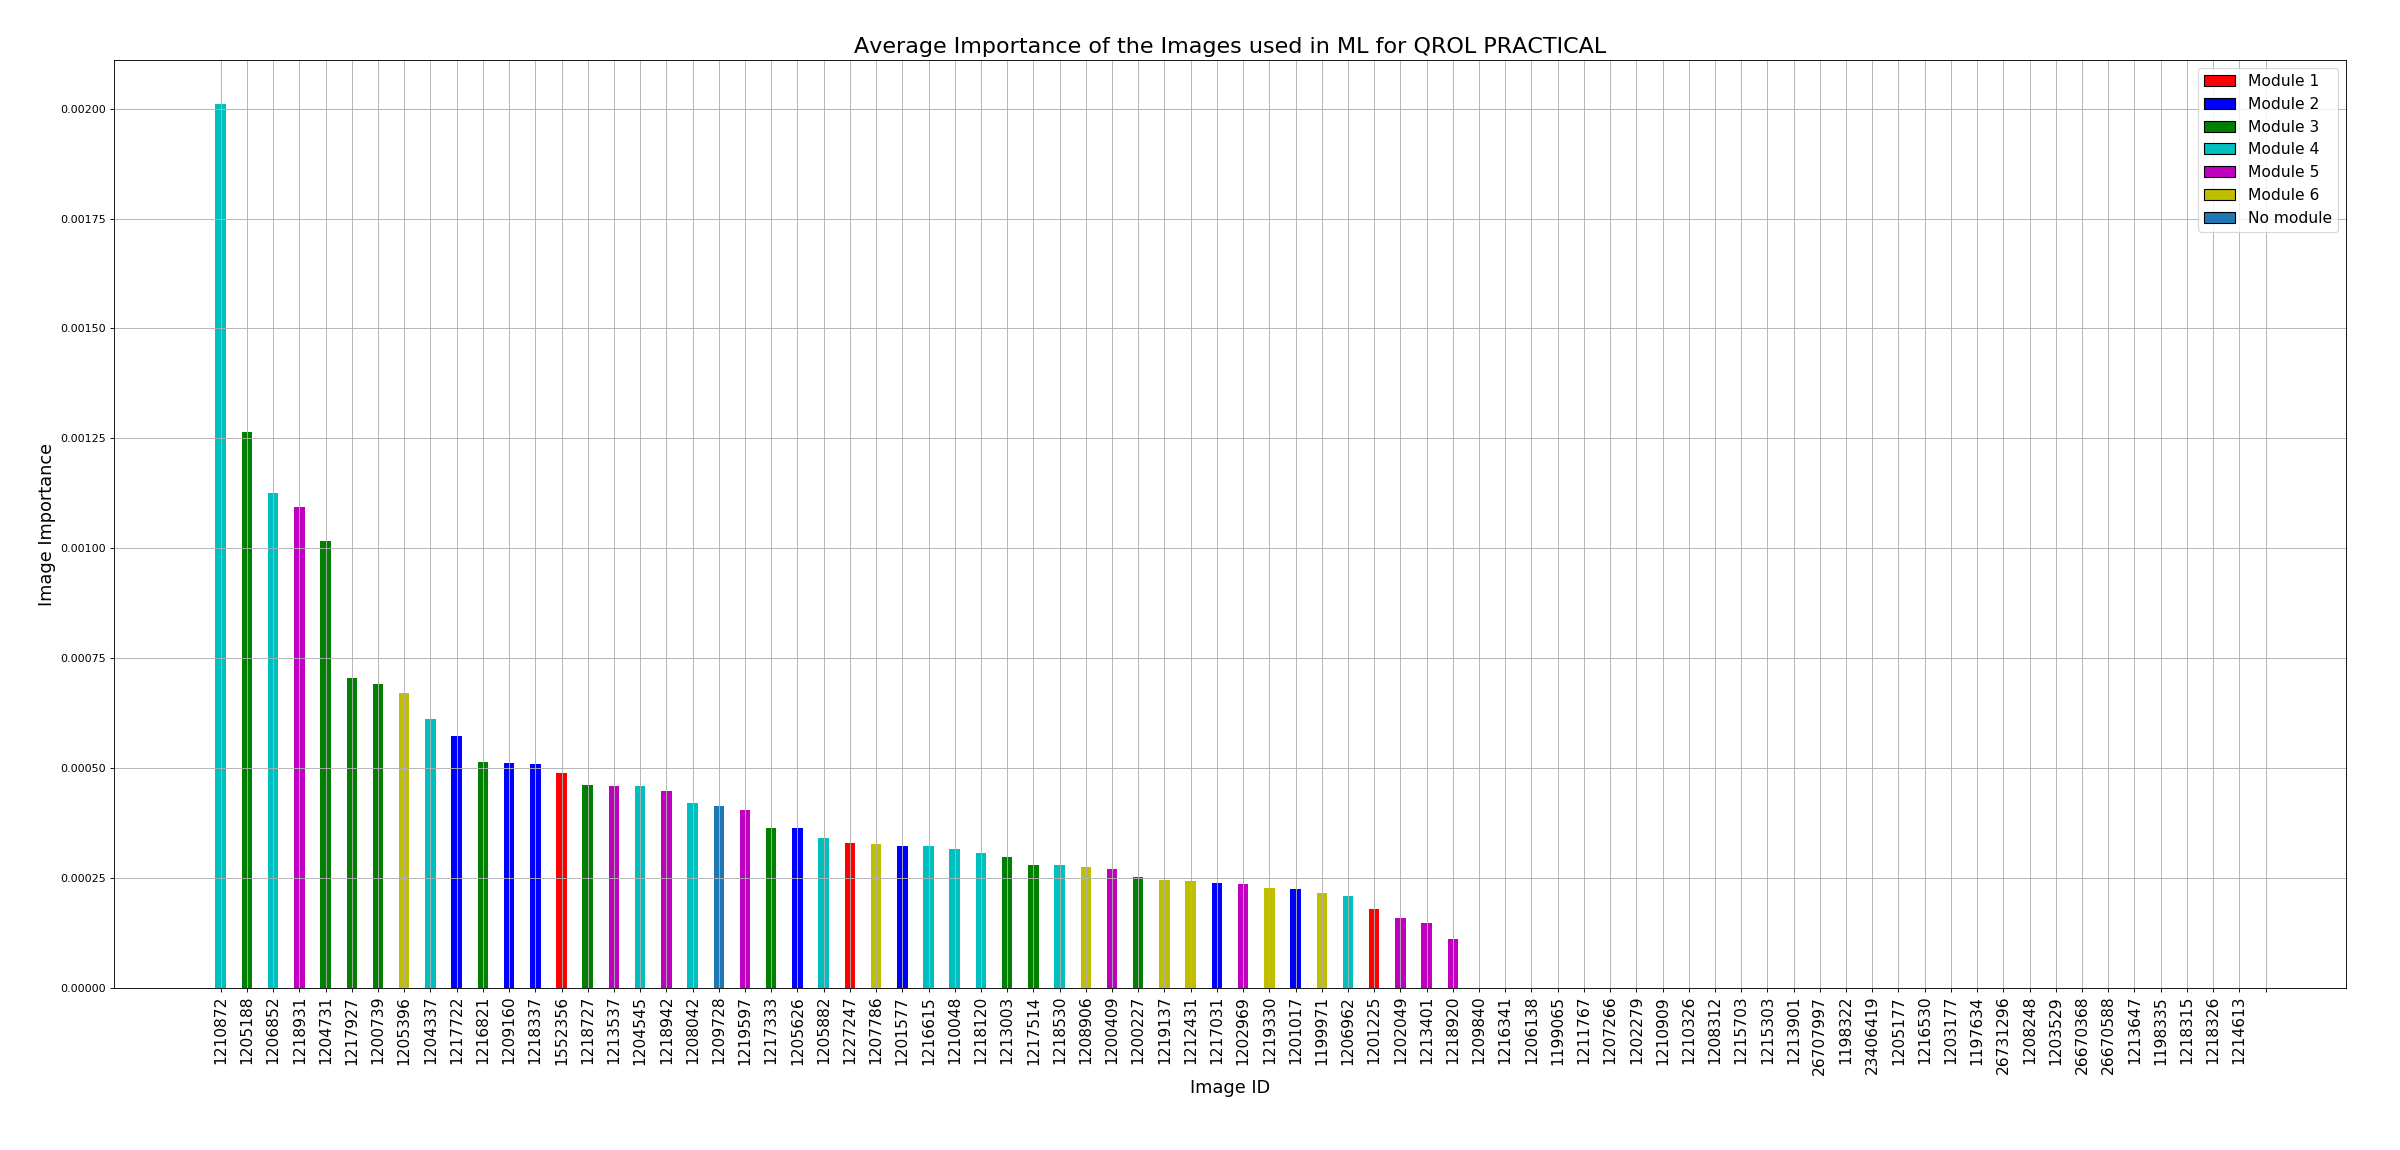
\includegraphics[width=.95\linewidth]{im_importance_QROL_PRACTICAL_2018-04-29_14_37_07.png}
      \caption{Image Importance for the QROL Practical}
      \label{fig:im_tp2}
      \end{figure}
      
      \begin{figure}[H]
      \centering
      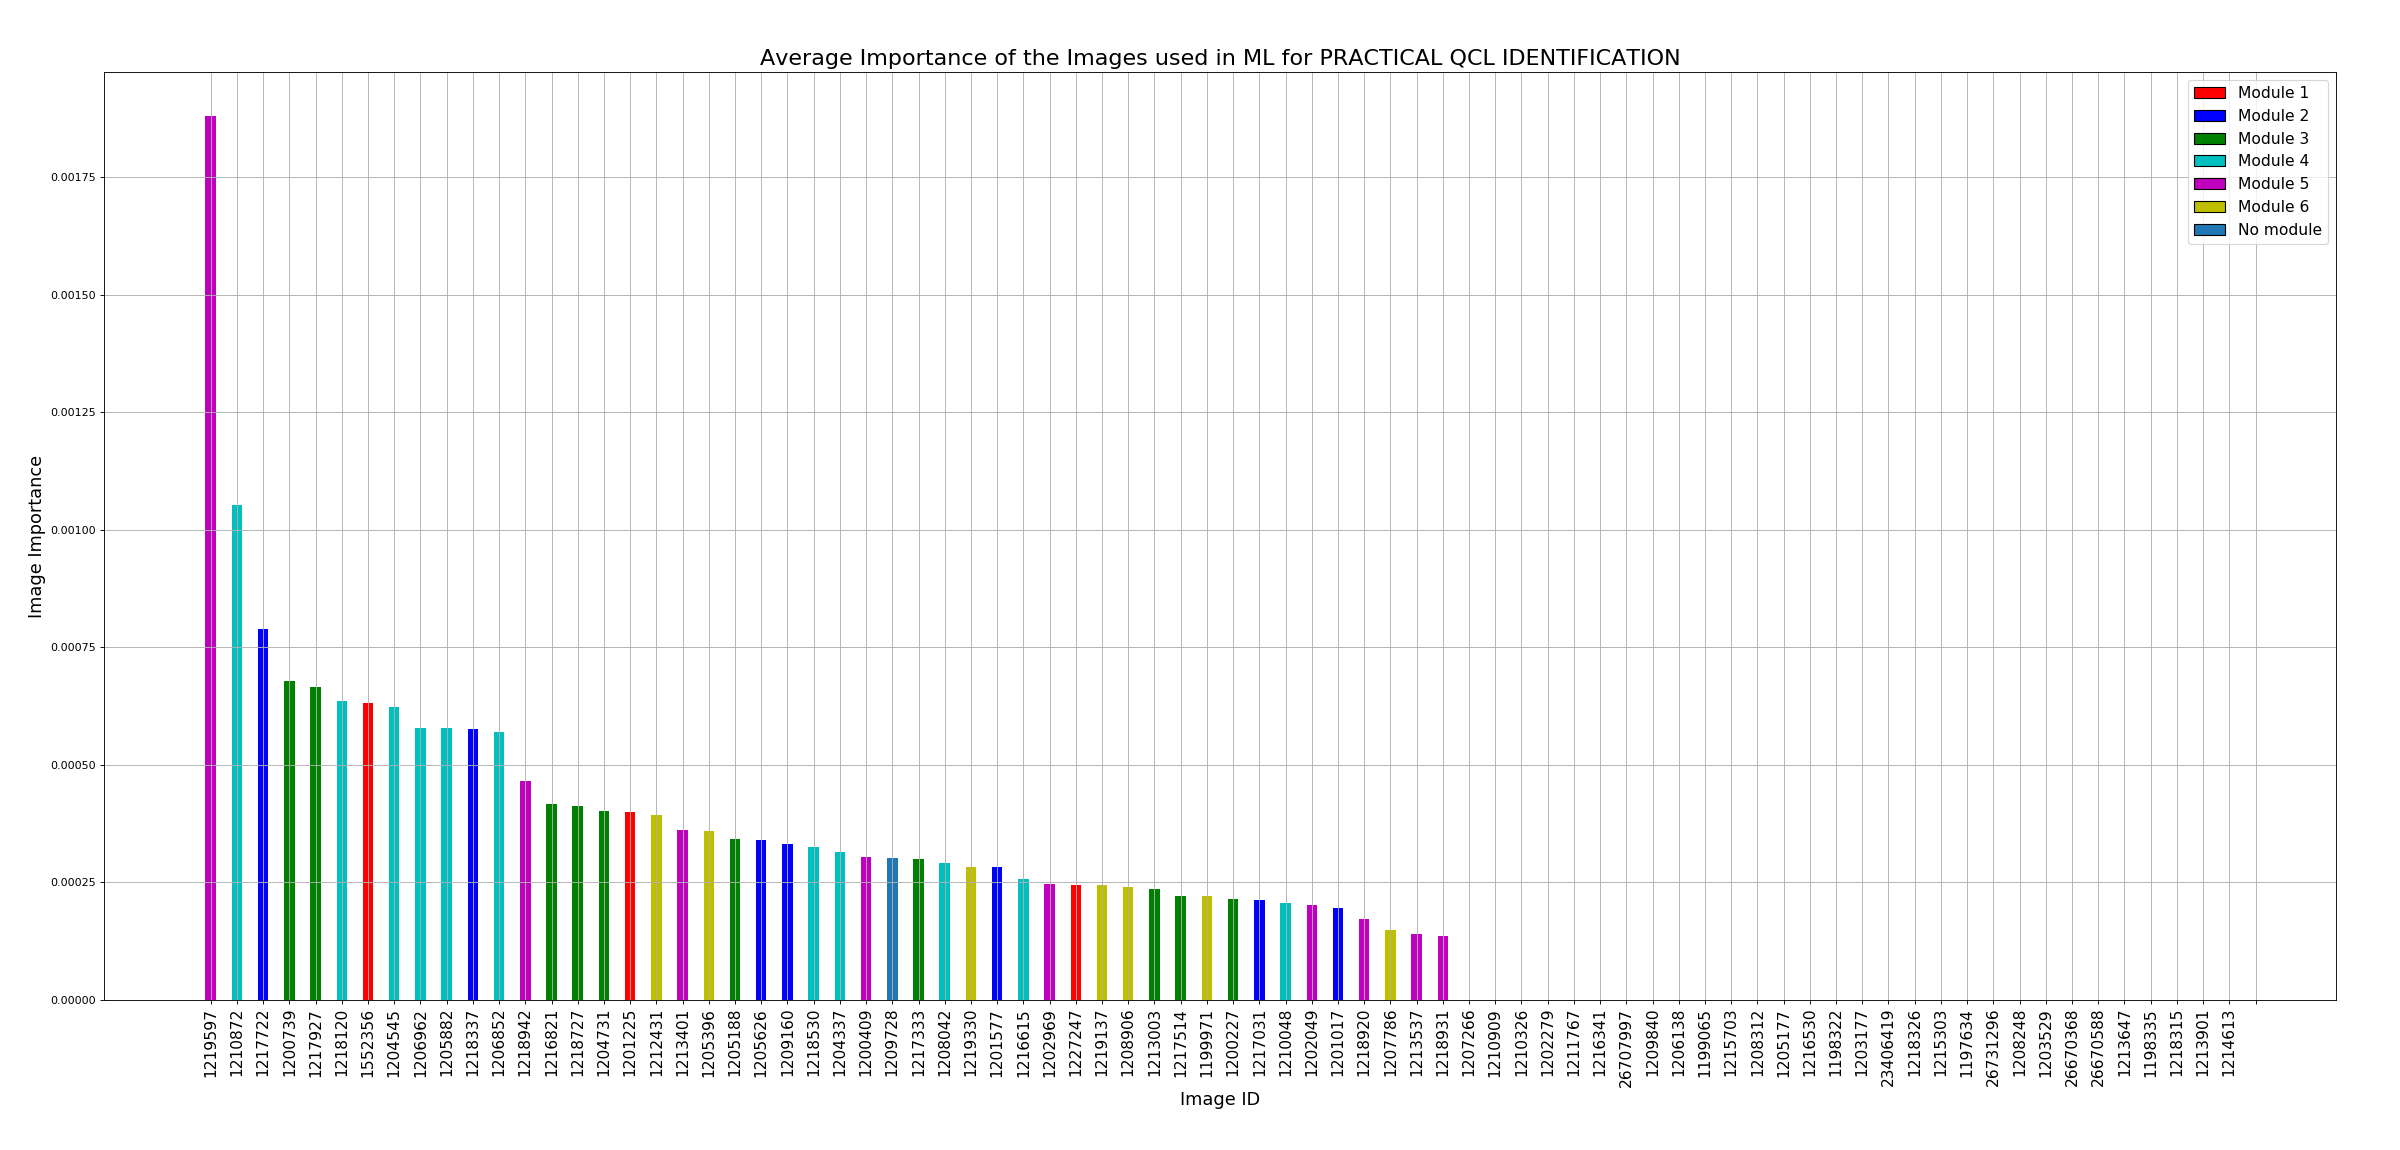
\includegraphics[width=.95\linewidth]{im_importance_PRACTICAL_QCL_IDENTIFICATION_2018-04-29_14_34_14.png}
      \caption{Image Importance for the QCL Identification}
      \label{fig:im_tp3}
      \end{figure}
      
      \begin{figure}[H]
      \centering
      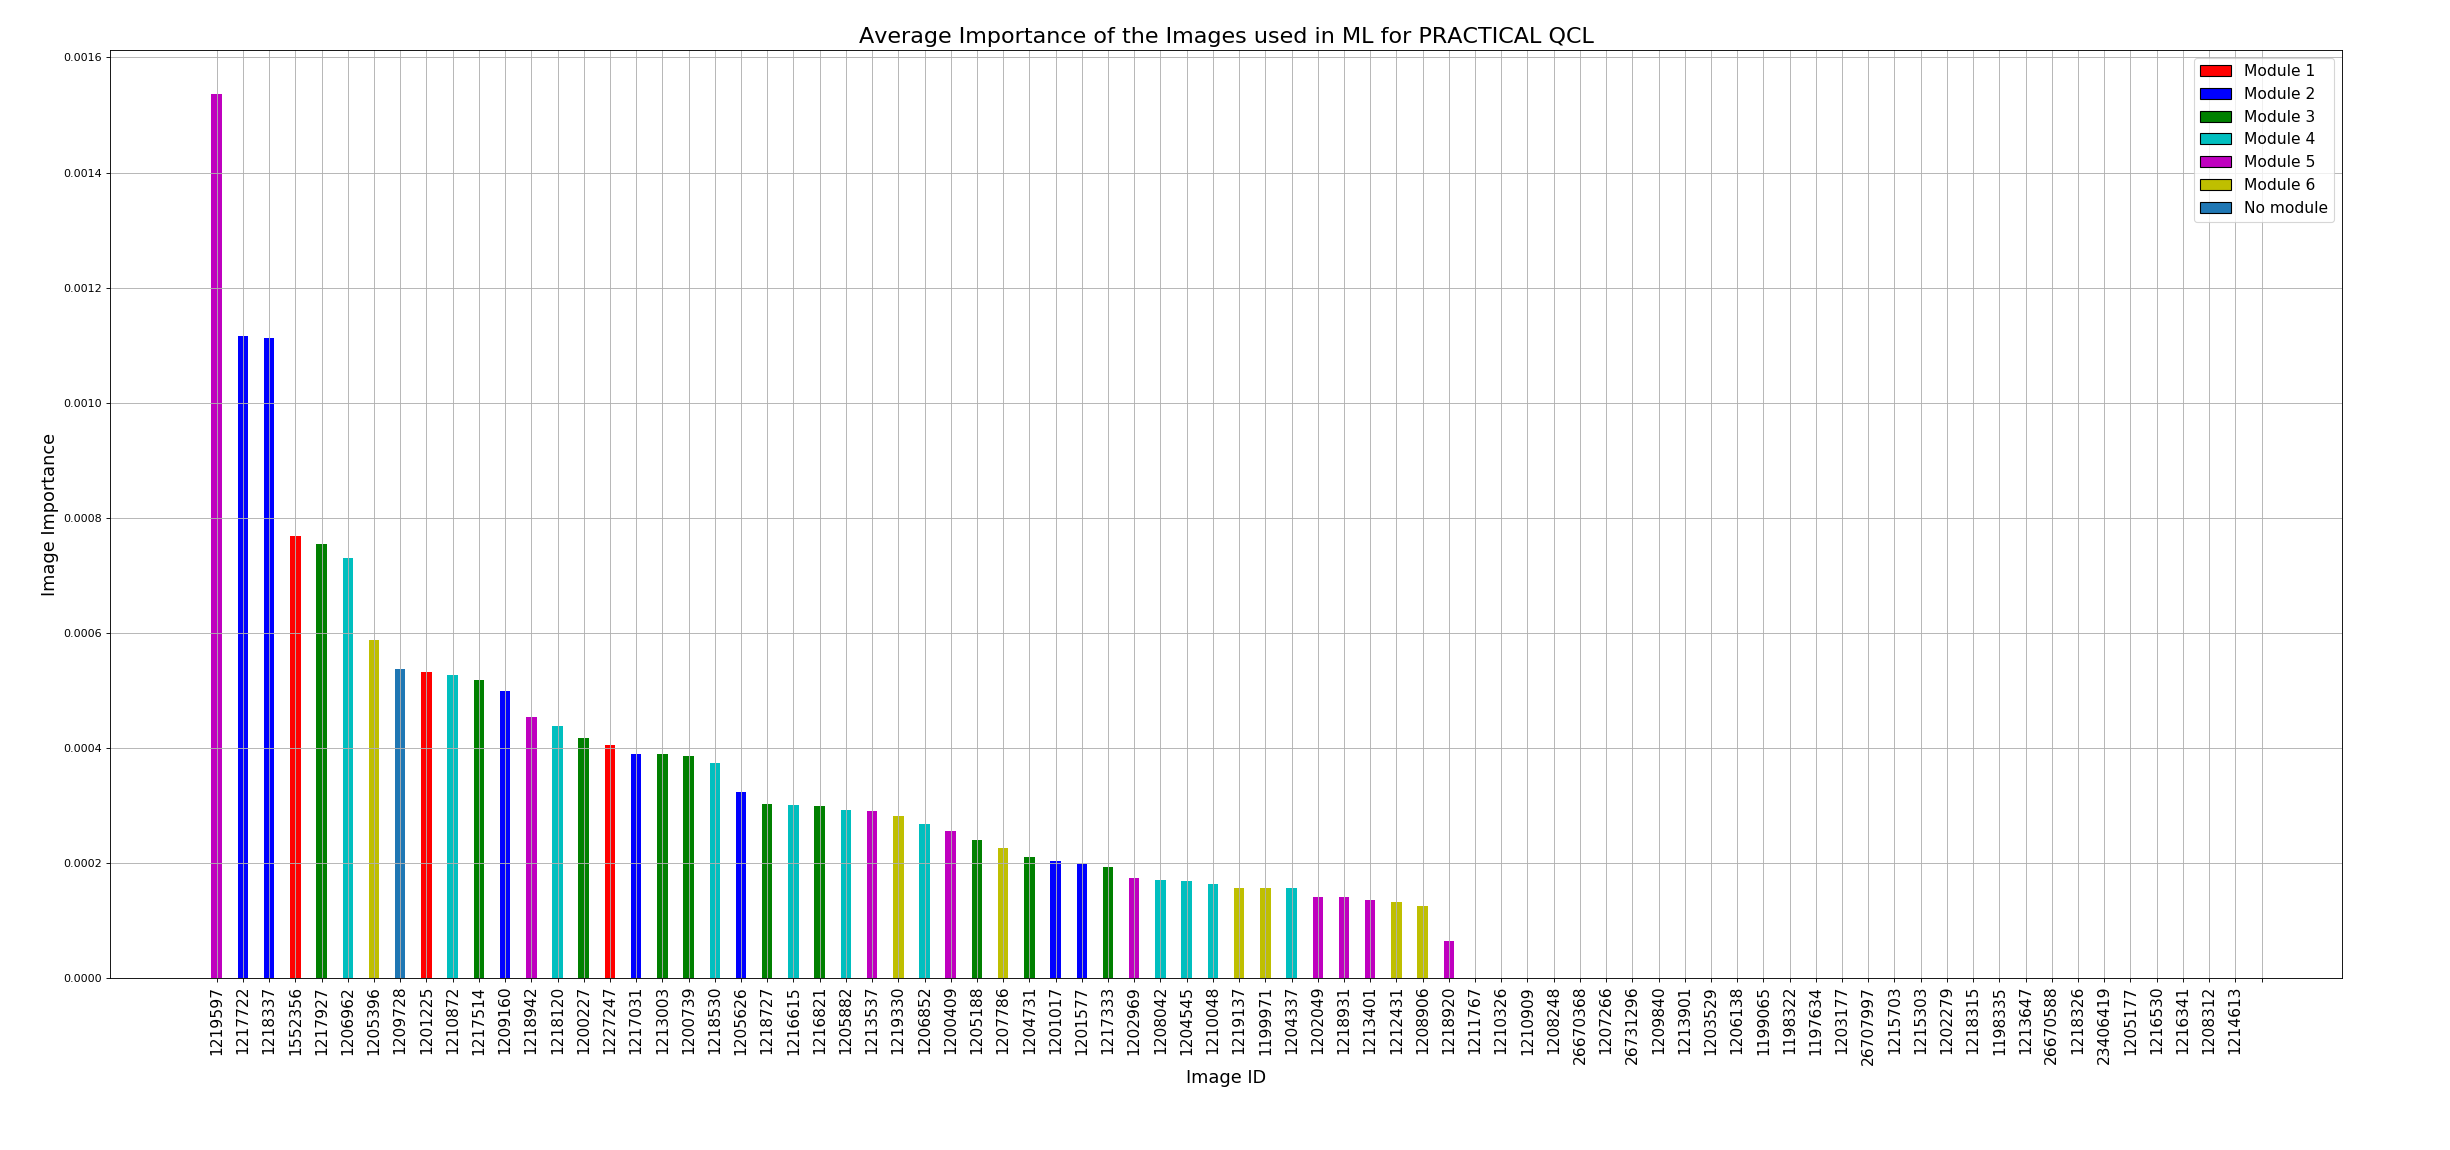
\includegraphics[width=.95\linewidth]{im_importance_PRACTICAL_QCL_2018-04-29_14_33_48.png}
      \caption{Image Importance for the QCL Incidence}
      \label{fig:im_tp4}
      \end{figure}

	It's hard to determine which modules were are more impactful as a whole.It seems that each module has at least one image that has a big impact on the result for each test.
	Like before, most these images are the ones dedicated to exercises.
	This supports the hypothesis that doing the exercises has a positive impact on the grades.
	But for example the image 1218120 does not appear at the top anymore.
	This shows that even tough the models follow the same patterns, it's still varies based on the contents of the exam.\\
    
    Sometimes it's interesting  to look for correlations between the expected result and some features.
    This helps to see its direct impact in estimating a grade.
    In fact, with most of the the features, a higher value should mean a better score.
    To test this, the Pearson Correlation was calculated for the top 6 features of the Practical QCM. (Figure \ref{fig:corr_tp})
      \begin{figure}[H]
      \centering
      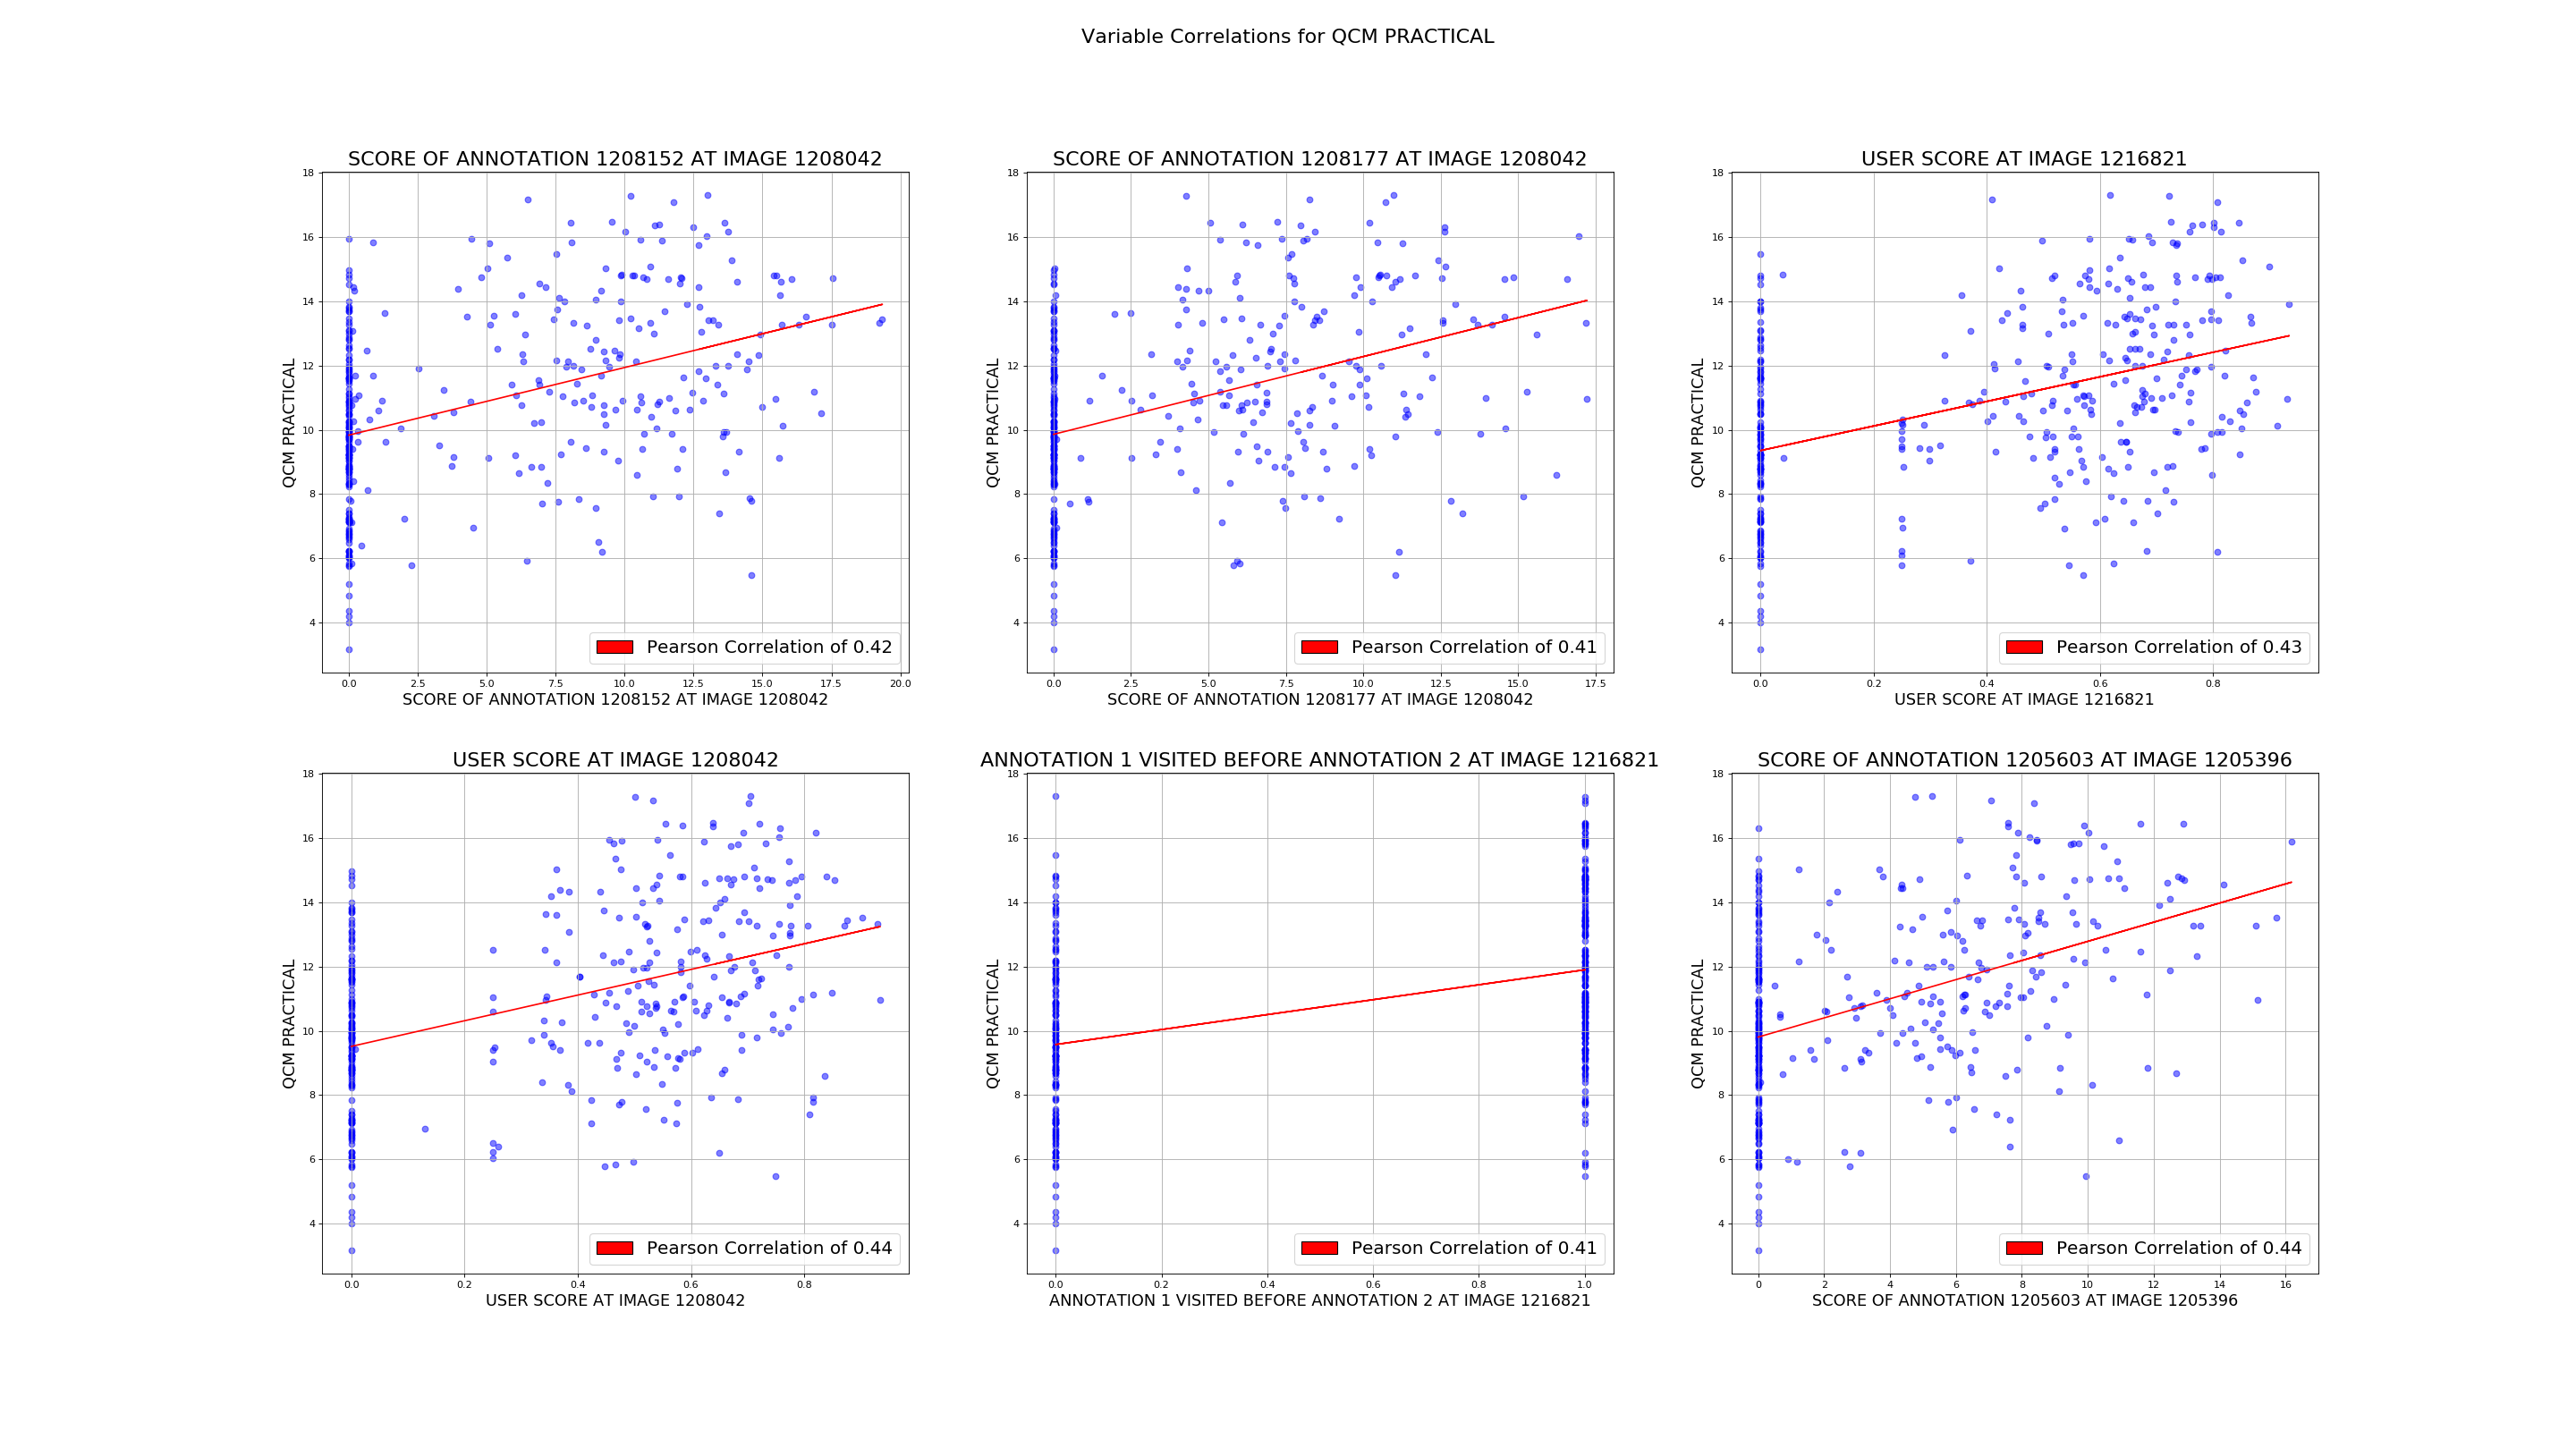
\includegraphics[width=.95\linewidth]{var_correlation_QCM_PRACTICAL_2018-04-29_14_38_14.png}
      \caption{Pearson Correlation}
      \label{fig:corr_tp}
      \end{figure}
    
   Most of these features are score features which in short tells the model how well the user viewed the image in regards to the annotations.
   Therefore a higher value means a better observation of all the annotations.
   This correlation means that the more time the student is focused on annotations, the more likely that student is to get a better grade.
   This could explain the somewhat good Pearson Correlation for these variables.\\
   
   After studying the results for the practical exams, a question that can be asked is whether or not this analysis can work on Theoretical Exam grades.
    
    \subsubsection{Theoretical Exam Grades}
        
        The same tests were launched for the theoretical grade results.
        The main difference for the theory portion is that there are no QCL tests and two QROL tests.
        The learning done on the QROL test results of the practical showed the worst results.
        Meanwhile the QCM provided the best results.
        This trend is likely to continue. (Figure \ref{fig:results_theo})
        
      \begin{figure}[H]
      \centering
      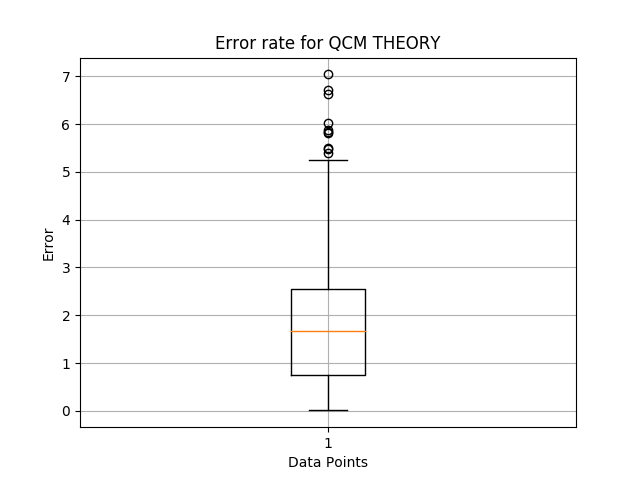
\includegraphics[width=.30\linewidth]{cv_boxplot_QCM_THEORY_2018-04-30_13_57_05.png}
      \includegraphics[width=.30\linewidth]{cv_boxplot_QROL1_THEORY_2018-04-30_13_40_50.png}
      \includegraphics[width=.30\linewidth]{cv_boxplot_QROL2_THEORY_2018-04-30_13_12_52.png}
      \\
      \ref{fig:results_theo}.1: Boxplots of the error values
      \\
      \vspace{0.5cm}
      \begin{tabular}{| l | c | c | c | c | c |}
      \hline
      & \tiny{Score} & \tiny{Median Score} & \tiny{Score Difference} & \tiny{Real Median Grade} & \tiny{Median Est.
      Grade}\\ \hline
      \tiny{QCM Theory} & \tiny{1.86} & \tiny{2.05} & \tiny{0.19} & \tiny{10.03} & \tiny{10.24}\\ \hline
      \tiny{QROL1 Theory} & \tiny{3.00} & \tiny{3.30} & \tiny{0.30} & \tiny{10.87} & \tiny{11.05}\\ \hline
      \tiny{QROL2 Theory} & \tiny{3.25} & \tiny{3.60} & \tiny{0.36} & \tiny{13.0} & \tiny{12.67}\\
      \hline
      \end{tabular}\\
      \vspace{0.5cm}
      \ref{fig:results_theo}.2: Discrete Results\\
      \vspace{0.3cm}
      \includegraphics[width=.30\linewidth]{cv_comp_QCM_THEORY_2018-04-30_13_57_05.png}
      \includegraphics[width=.30\linewidth]{cv_comp_QROL1_THEORY_2018-04-30_13_40_50.png}
  	  \includegraphics[width=.30\linewidth]{cv_comp_QROL2_THEORY_2018-04-30_13_12_52.png}
      \\
      \ref{fig:results_theo}.3: Actual grades compared to Predicated grades
      \caption{Results from cross-validation of the practical tests}
      \label{fig:results_theo}
    \end{figure}
    
    As predicted, the QCM yielded the best scores while the QROL provided sub par scores.
    The assumptions made based off of the practical exams were correct.
    The Extra Trees has an easier time predicting QCM exams.
    But in this case, the QCM grades has a lower variance then the QROL.\\


    The following figures show the feature importance for their respective model (Figures \ref{fig:var_th1}, \ref{fig:var_th2}, and \ref{fig:var_th3}).

     \begin{figure}[H]
      \centering
      \includegraphics[width=.95\linewidth]{var_importance_QCM_THEORY_2018-05-02_20_53_18.png}
      \caption{Feature Importance for the QCM Theory}
      \label{fig:var_th1}
      \end{figure}
      
      \begin{figure}[H]
      \centering
      \includegraphics[width=.95\linewidth]{var_importance_QROL1_THEORY_2018-05-02_20_54_23.png}
      \caption{Feature Importance for the QROL1 Theory}
      \label{fig:var_th2}
      \end{figure}
      
      \begin{figure}[H]
      \centering
      \includegraphics[width=.95\linewidth]{var_importance_QROL2_THEORY_2018-05-02_20_53_44.png}
      \caption{Feature Importance for the QROL2 Theory}
      \label{fig:var_th3}
      \end{figure}    

    As usual, the scores are the most prominent features for all the theoretical exercises.
    It's interesting to note some differences with the practical exercices.
    This includes features that are associated to the time worked.
    It would not be too much of a stretch to theorize that studying with Cytomine during certain time periods, the student would assimilate more information.
    For example, when working after 2AM, the students may be more tired and they might retain less information.\\


    As for images themselves, the QROL questions are more specific so certain images may be the centerpiece. (Figures \ref{fig:im_th1}, \ref{fig:im_th2}, and \ref{fig:im_th3})

     \begin{figure}[H]
      \centering
      \includegraphics[width=.95\linewidth]{im_importance_QCM_THEORY_2018-05-02_20_53_22.png}
      \caption{Image Importance for the QCM Theory}
      \label{fig:im_th1}
      \end{figure}
      
      \begin{figure}[H]
      \centering
      \includegraphics[width=.95\linewidth]{im_importance_QROL1_THEORY_2018-05-02_20_54_25.png}
      \caption{Image Importance for the QROL1 Theory}
      \label{fig:im_th2}
      \end{figure}
      
      \begin{figure}[H]
      \centering
      \includegraphics[width=.95\linewidth]{im_importance_QROL2_THEORY_2018-05-02_20_53_48.png}
      \caption{Image Importance for the QROL2 Theory}
      \label{fig:im_th3}
      \end{figure}    

    As predicted, some images and modules are more relevant then others.
    For the QROL1, it seems that the question was associated information that the students learned from the modules 5 and 6.
    The image 1208906 which is an image used for learning is the most important.
    This is contrasted by the QROL1 question where the more important images are associated to the earlier modules (1 and 3).
    In this case, the image 1218727 was the most impactful.
    This image was given more as an exercise image as opposed to the previous one.
    As for the QCM, the image 1208906 also stood out.
    It's possible that, there's more educational interest behind this image.

    \subsubsection{Global Grades}

    The next objective is to study these grades as a whole.
    This includes the total theoretical grades, the total practical grade, and the exam as a whole. (Figure \ref{fig:results_tot})

    
      \begin{figure}[H]
      \centering
      \includegraphics[width=.30\linewidth]{cv_boxplot_TOTAL_TP_2018-04-27_19_24_46.png}
      \includegraphics[width=.30\linewidth]{cv_boxplot_TOTAL_THEORY_2018-04-30_13_53_15.png}
      \includegraphics[width=.30\linewidth]{cv_boxplot_GLOBAL_GRADE_2018-04-30_13_48_59.png}
      \\
      \ref{fig:results_tot}.1: Boxplots of the error values
      \\
      \vspace{0.5cm}
      \begin{tabular}{| l | c | c | c | c | c |}
      \hline
      & \tiny{Score} & \tiny{Median Score} & \tiny{Score Difference} & \tiny{Real Median Grade} & \tiny{Median Est.
      Grade}\\ \hline
      \tiny{Total Practical} & \tiny2.12 & \tiny{2.59} & \tiny{0.47} & \tiny{10.80} & \tiny{11.06}\\ \hline
      \tiny{Total Theory} & \tiny{2.03} & \tiny{2.34} & \tiny{0.31} & \tiny{10.79} & \tiny{10.86}\\ \hline
      \tiny{Global Grade} & \tiny{1.95} & \tiny{2.37} & \tiny{0.42} & \tiny{10.72} & \tiny{10.95}\\
      \hline
      \end{tabular}\\
      \vspace{0.5cm}
      \ref{fig:results_tot}.2: Discrete Results\\
      \vspace{0.3cm}
      \includegraphics[width=.30\linewidth]{cv_comp_TOTAL_TP_2018-04-27_19_24_46.png}
      \includegraphics[width=.30\linewidth]{cv_comp_TOTAL_THEORY_2018-04-30_13_53_15.png}
  	  \includegraphics[width=.30\linewidth]{cv_comp_GLOBAL_GRADE_2018-04-30_13_48_59.png}
      \\
      \ref{fig:results_tot}.3: Actual grades compared to Predicated grades
      \caption{Results from cross-validation of the exam results}
      \label{fig:results_tot}
    \end{figure}
    
    As a whole, there's a mean absolute error of about 2.
    Overall, still not the best results.
    An interesting observation is that the learning algorithm has a easier time predicting theoretical grades over practical grades.
    As using Cytomine is overall a practical activity, the fact predicting theoretical grades works just as well can possibly imply that students can retain theoretical concepts with Cytomine.\\

    Observing what behaviors lead to this grade can prove useful : (Figures \ref{fig:var_tot1}, \ref{fig:var_tot2}, and \ref{fig:var_tot3})

      \begin{figure}[H]
      \centering
      \includegraphics[width=.95\linewidth]{var_importance_TOTAL_TP_2018-04-29_14_37_37.png}
      \caption{Feature Importance for the Practical}
      \label{fig:var_tot1}
      \end{figure}
      
      \begin{figure}[H]
      \centering
      \includegraphics[width=.95\linewidth]{var_importance_TOTAL_THEORY_2018-05-02_23_31_54.png}
      \caption{Feature Importance for the Theory}
      \label{fig:var_tot2}
      \end{figure}
      
      \begin{figure}[H]
      \centering
      \includegraphics[width=.95\linewidth]{var_importance_GLOBAL_GRADE_2018-05-02_20_56_11.png}
      \caption{Feature Importance for the Total}
      \label{fig:var_tot3}
      \end{figure}   

    Overall, the most impactful features are often associated to the students' performance scores for all the models.
    This indicator that the student followed the instructions has a notable impact on the results.
    Also, module features are also much less impactful than their regular counterparts.\\

    As for the images themselves the results are : (Figures \ref{fig:im_tot1}, \ref{fig:im_tot2}, and \ref{fig:im_tot3})
      
      \begin{figure}[H]
      \centering
      \includegraphics[width=.95\linewidth]{im_importance_TOTAL_TP_2018-04-29_14_37_40.png}
      \caption{Image Importance for the total Practical}
      \label{fig:im_tot1}
      \end{figure}

      \begin{figure}[H]
      \centering
      \includegraphics[width=.95\linewidth]{im_importance_TOTAL_THEORY_2018-05-02_23_31_57.png}
      \caption{Image Importance for the total Theory}
      \label{fig:im_tot2}
      \end{figure}

      \begin{figure}[H]
      \centering
      \includegraphics[width=.95\linewidth]{im_importance_GLOBAL_GRADE_2018-05-02_20_56_13.png}
      \caption{Image Importance for the Global Grade}
      \label{fig:im_tot3}
      \end{figure}

    For the most part, the important images are similar to those of all the individual tests put together.
    So as a whole, there's a sizable set of images that have a high impact on the grades predicted.
    
    \subsubsection{Learning with additional Information}
    %todo guess theory with practical
    %todo guess practical with theory.
    
    
    
\section{Discussion} \label{Discussion}

    \subsection{Negatives}

        First of all, the results obtained from the Machine Learning were subpar.
        A mean Absolute error of around 2.0 out of 20 is 10\% of the range which is not great.
        The main cause of which is the small data set of 395 students.
        If it was possible to group people up based on habits and patterns, 395 students would not be enough for such study.
        It's still important to stay skeptical because every person is unique.
        Some people have a much easier time learning than others.
        In such cases, the student may not need much time to understand the concepts provided by Cytomine.
        Therefore, there there are less recorded positions and actions.
        In other case, the exact opposite.
        When on Cytomine, the analyst can't be in the person's head when using the application.
        The student can go on the website and retain nothing.
        Also, the Gaze data may not be perfectly accurate.
        Without sensors that observe the user's eye movements, it's very impractical to track Gaze data.
        In most cases, a person is usually focused on or near the center of the screen.
        It's possible that they can focus more towards a corner.
        In it's current state, corners have a lower value from the calculated Gaussian distribution.
        It's also worth to mention again that positions are still recorded even when the window is not active.
        Since this issue is not easy to resolve without losing information, it also may lead to some inaccuracies.
        It's also important to note that much information is contained in the course itself.
        The course contains numerous examples of cells and tissues that is also found on Cytomine.
        It's entirely possible that students can ignore Cytomine for the most part and just learn from the course's Syllabus.\\


        But overall it may be a good thing that the results were not so great.
        It is important to keep in mind that this study is not used to encourage students to follow the directions to the letter.
        The students should be free to work on their course the way they see fit.
        If they were to fail, it is their own problem.
        It's also important to encourage different styles and methods, and not force a particular way of thinking.
        This is why the Annotation visit order features were not very impactful.
        If those variables were more impactful and the results were better, it could have implied that visiting annotations in a specific order would be important to passing the exam.
        Overall the goal is not to try and dictate how the students work.

\section{Conclusion}
\end{document}